\باب{سمتی تکملی علم الاحصاء۔ تکمل کے مسئلے}
تکمل سے آپ بخوبی واقف ہیں جس کو \اصطلاح{سمتی تکملی علم الاحصاء}\حاشیہب{vector calculus} وسعت دیتا ہے۔یوں منحنی پر تکمل، جسے \اصطلاح{خطی تکمل}\حاشیہب{line integral} کہتے ہیں، سطح پر تکمل جسے \اصطلاح{سطحی تکمل}\حاشیہب{surface integral} کہتے ہیں اور حجم پر تکمل جسے \اصطلاح{حجمی تکمل}\حاشیہب{volume integral} کہتے ہیں،  حاصل کیا جا سکتا ہے۔مزید ایک قسم کی تکمل کا دوسری قسم کی تکمل میں تبادلہ کیا جا سکتا ہے۔ایسا کرنے سے بعض اوقات نسبتاً آسان تکمل حاصل ہوتا ہے۔یوں سطح میں  \اصطلاح{مسئلہ گرین}\حاشیہب{Green's theorem} کی مدد سے خطی تکمل کو دو درجی تکمل میں یا دو درجی تکمل کو خطی تکمل میں تبدیل کیا جا سکتا ہے۔ \اصطلاح{گاوسی مسئلہ ارتکاز}\حاشیہب{Gauss's convergence theorem} کی مدد سے حجمی تکمل کو سطحی تکمل یا سطحی تکمل کو حجمی تکمل میں تبدیل کیا جاتا ہے۔\اصطلاح{مسئلہ سٹوکس}\حاشیہب{Stoke's theorem} کی مدد سے تین درجی تکمل کو خطی تکمل یا خطی تکمل کو تین درجی تکمل میں تبدیل کیا جا سکتا ہے۔

سمتی تکملی الاحصاء کا انجینئری، طبیعیات، ٹھوس میکانیات، سیالی میکانیات اور دیگر میدان میں اہم کردار پایا جاتا ہے۔

%===============
\حصہ{خطی تکمل}
 درج ذیل  تفاعل \عددی{f} کی \عددی{x} محور پر \عددی{x=a} تا \عددی{x=b} قطعی تکمل ہے
\begin{align}\label{مساوات_سمتی_تکمل_قطعی}
\int_a^b f(x)\dif x
\end{align}
جہاں وقفہ \عددی{a} اور \عددی{b} کے درمیان  ہر نقطے پر \عددی{f} معین ہے۔ خطی تکمل میں \عددی{f} کا تکمل سطح میں (یا فضا میں) منحنی \عددی{C} پر حاصل کیا جاتا ہے جہاں \عددی{C} کے ہر نقطے پر \عددی{f} معین ہے۔

خطی تکمل کی تعریف عین قطعی تکمل کی تعریف کی مانند ہے۔خطی تکمل کچھ یوں ہے۔

ہم فضا میں منحنی \عددی{C} لیتے ہیں اور اس پر ایک رخ کو \اصطلاح{مثبت سمت} کہتے ہیں۔یوں منحنی پر الٹ چلتے ہوئے منفی سمت حاصل ہو گی۔مثبت سمت میں چلتے ہوئے منحنی پر ابتدائی نقطے کو \عددی{A} اور اختتامی نقطے کو \عددی{B} کہتے ہیں۔ جیسا شکل \حوالہ{شکل_سمتی_تکمل_سمت_بند_منحنی}-ب میں دکھایا گیا ہے ابتدائی نقطہ اور اختتامی نقطہ ہم مقام ہو سکتے ہیں۔ایسی صورت میں \عددی{C} بند راہ کہلاتا ہے۔ہم فرض کرتے ہیں کہ \عددی{C} سادہ منحنی (حصہ \حوالہ{حصہ_الاحصاء_منحنی}) ہے  جس کو
\begin{align}\label{مساوات_سمتی_تکمل_راہ_الف}
\bM{r}(s)=x(s)\bM{i}+y(s)\bM{j}+z(s)\bM{k}\quad \quad \quad (a\le s\le b)
\end{align}
 ظاہر کرتی ہے [جہاں \عددی{s} منحنی کی لمبائی قوس ہے (حصہ \حوالہ{حصہ_الاحصاء_لمبائی_قوس})] اور پورے \عددی{C} پر \عددی{\bM{r}(s)} استمراری ہے جس کا (پورے \عددی{C} پر)   تفرق \عددی{\bM{r}'} موجود ہے اور یہ تفرق غیر صفر سمتیہ ہے۔اس طرح \عددی{C} \اصطلاح{ہموار منحنی}\فرہنگ{ہموار!منحنی}\فرہنگ{منحنی!ہموار}\حاشیہب{smooth curve}\فرہنگ{smooth!curve} کہلائے گی یعنی \عددی{C} کے ہر نقطے پر \عددی{C} کا منفرد مماس پایا جاتا ہے  اور منحنی پر چلنے سے مماس کی سمت میں تبدیلی استمراری ہوتی ہے۔
\begin{figure}
\centering
\begin{subfigure}{0.5\textwidth}
\centering
\begin{tikzpicture}
\draw[->-=0.5](0,0)node[ocirc]{}node[right]{$A$} to [out=135,in=0]++(-1,2)node[ocirc]{}node[left]{$B$};
\draw(-0.3,1)node[right]{$C$};
\end{tikzpicture}
\caption*{(الف)}
\end{subfigure}%
\begin{subfigure}{0.5\textwidth}
\centering
\begin{tikzpicture}
\draw[->-=0.2](0,0) to [out=0,in=-90]++(1,1) to [out=90,in=-90]++(0.5,1)node[left]{$C$} to [out=90,in=0]++(-0.5,0.5) to [out=180,in=90]++(-1.5,-1)node[ocirc]{}node[left]{$A$}node[right]{$B$} to [out=-90,in=180] (0,0);
\end{tikzpicture}
\caption*{(ب)}
\end{subfigure}%
\caption{سمت بند منحنی}
\label{شکل_سمتی_تکمل_سمت_بند_منحنی}
\end{figure}

فرض کریں کہ \عددی{f(x,y,z)} متغیر \عددی{s} کا ایسا استمراری تفاعل ہے  جو (کم از کم) \عددی{C} کے ہر نقطے پر معین ہے۔ہم \عددی{C} کو بے قاعدہ طریقے سے \عددی{n} عدد ٹکڑوں میں تقسیم کرتے ہیں (شکل \حوالہ{شکل_سمتی_تکمل_راہ_کی_تقسیم})۔یوں ہر ٹکڑے کی لمبائی مختلف ہو سکتی ہے۔ہم ابتدائی سر سے شروع کرتے ہوئے ان ٹکڑوں کے سروں کو \عددی{P_0\, (=A)}، \عددی{P_1}، \عددی{P_2}، \نقطے \عددی{P_n\,(=B)} سے اور \عددی{s} کی مطابقتی قیمتوں کو
\begin{align*}
s_0\,(=a)<s_1<s_2<\dots<s_n\,(=b)
\end{align*}
سے ظاہر کرتے ہیں۔ہم ہر ٹکڑے پر بے قاعدگی سے کوئی نقطہ چنتے ہیں مثلاً \عددی{P_0} اور \عددی{P_1} کے درمیان ٹکڑے پر ہم نقطہ \عددی{Q_1} چنتے ہیں، \عددی{P_1} اور \عددی{P_2} کے درمیان ٹکڑے پر ہم نقطہ \عددی{Q_2} چنتے ہیں وغیرہ وغیرہ۔یوں ہر ٹکڑے پر نقطہ باقی ٹکڑوں پر نقطوں سے ضروری نہیں کہ کوئی مشابہت رکھتا ہو۔ ان نقطوں پر \عددی{f} کی قیمتوں کو لیتے ہوئے ہم مجموعہ
\begin{align}\label{مساوات_خطی_تکمل_تعریف_بطور_مجموعہ}
J_n=\sum_{m=1}^{n} f(x_m,y_m,z_m)\Delta s_m
\end{align}
لیتے ہیں جہاں \عددی{x_m}، \عددی{y_m}، \عددی{z_m} نقطہ \عددی{Q_m} کے محدد ہیں اور \عددی{\Delta s_m} اس ٹکڑے کی لمبائی ہے جس پر \عددی{Q_m} واقع ہے۔
\begin{align*}
\Delta s_m=s_m-s_{m-1}
\end{align*}
ہم اس طرح کے مجموعے مکمل بے قاعدگی سے \عددی{n=2,3,\cdots} کے لئے یوں حاصل کرتے ہیں کہ جیسے جیسے \عددی{n} کی قیمت لامتناہی تک پہنچے، \عددی{\Delta s} کی زیادہ سے زیادہ قیمت صفر تک پہنچتی ہو۔یوں ہمیں مجموعوں کا تسلسل \عددی{J_2,J_3,\cdots} ملتا ہے۔ اس تسلسل کی حد کو \عددی{C} پر \عددی{A} تا \عددی{B} تفاعل \عددی{f} کی \اصطلاح{خطی تکمل}\فرہنگ{خطی!تکمل}\فرہنگ{تکمل!خطی}\حاشیہب{line integral}\فرہنگ{integral!line} کہتے ہیں جس کو درج ذیل سے ظاہر کیا جاتا ہے۔
\begin{align*}
\int_C f(x,y,z)\dif s
\end{align*}
منحنی \عددی{C} کو \اصطلاح{تکمل کی راہ}\فرہنگ{تکمل!راہ}\فرہنگ{راہ!تکمل} کہتے ہیں جبکہ \عددی{f(x,y,z)} کو \اصطلاح{متکمل}\فرہنگ{متکمل}\حاشیہب{integrand}\فرہنگ{integrand} کہتے ہیں۔
%
\begin{figure}
\centering
\begin{tikzpicture}
%\draw[thick,step=1](0,0) grid (6,3);
%\draw[thin,gray,step=0.1](0,0) grid (6,3);
%
\draw(0,0)node[ocirc]{}node[left]{$A=P_0$} to [out=60,in=-70] (5,3)node[ocirc]{}node[right]{$B=P_n$};
%
\draw(0.4,0.6)--++(-45:0.2)node[shift={(-45:0.3)}]{$P_1$};
\draw(1.1,1)--++(-60:0.2)node[shift={(-60:0.3)}]{$P_2$};
\draw(1.6,1.2)--++(-70:0.2);
\draw(2.2,1.3)--++(-75:0.2)node[shift={(-75:0.3)}]{$P_{m-1}$};
\draw(3.2,1.5)--++(-80:0.2)node[shift={(-80:0.3)}]{$P_{m}$};
\draw(3.6,1.6)--++(-70:0.2);
\draw(4,1.7)--++(-65:0.2);
\draw(4.9,2.2)--++(-45:0.2)node[shift={(-45:0.35)}]{$P_{n-1}$};
\draw(2.6,1.32)node[circle,inner sep=0pt,minimum size=3pt,fill=black,label=above:{$Q_m$}]{};
\end{tikzpicture}
\caption{\عددی{C} کی ٹکڑوں میں تقسیم}
\label{شکل_سمتی_تکمل_راہ_کی_تقسیم}
\end{figure}

چونکہ \عددی{f} کو استمراری فرض کیا گیا اور \عددی{C} ہموار ہے لہٰذا یہ حد موجود ہو گا جس کی قیمت پر ٹکڑوں کی چناؤ اور ٹکڑوں پر نقطوں کی چناؤ کا کوئی اثر نہیں ہو گا۔ \عددی{C} پر کسی بھی نقطہ \عددی{P} کا تعین لمبائی قوس \عددی{s} سے کیا جاتا ہے۔یوں \عددی{A} اور \عددی{B} کا تعین مطابقتی \عددی{s=a} اور \عددی{s=b} سے کیا جائے گا لہٰذا ہم درج ذیل لکھ سکتے ہیں
\begin{align}\label{مساوات_خطی_تکمل_سے _قطعی_الف}
\int_C f(x,y,z)\dif s=\int_a^b f[x(s),y(s),z(s)]\dif s
\end{align}
جو قطعی تکمل ہے۔ہم جانتے ہیں کہ قطعی تکمل  بھی تسلسل \عددی{J_2,J_3,\cdots} کی حد کو کہتے ہیں جس کی قیمت پر نا تو ٹکڑوں کی تقسیم اور نا ہی ٹکڑوں پر نقطوں کی چنائی کا کوئی اثر پایا جاتا ہے۔مثال \حوالہ{مثال_سمتی_تکمل_رقبہ_اور_تکمل} میں مزید تفصیل دی گئی ہے۔

%================================
\ابتدا{مثال}\شناخت{مثال_سمتی_تکمل_رقبہ_اور_تکمل}\quad تکمل کی قیمت پر ٹکڑوں کی چناؤ اور ٹکڑوں پر نقطوں کے چناؤ کا کوئی اثر نہیں پایا جاتا ہے\\
آئیں دیکھتے ہیں کہ تکمل کی قیمت پر راہ کی ٹکڑوں میں تقسیم اور ان ٹکڑوں پر نقطوں کی چنائی کا کوئی اثر کیوں نہیں پایا جاتا ہے۔شکل \حوالہ{شکل_مثال_سمتی_تکمل_رقبہ_اور_تکمل} میں تفاعل \عددی{y=f(x)} دکھایا گیا ہے جس کا ابتدائی نقطہ \عددی{A} اور اختتامی نقطہ \عددی{B} ہے۔ ان نقطوں کے درمیان تفاعل کو بے قاعدہ ٹکڑوں میں تقسیم کیا گیا ہے۔
\begin{figure}
\centering
\begin{tikzpicture}
%\draw[step=1,thick](0,0) grid (6,2);
%\draw[step=0.1,gray,thin](0,0) grid (6,2);
%
\draw(0,0)--++(6.5,0)node[below]{$x$};
\draw(0,0)--++(0,2.5)node[left]{$y$};
%
\draw[name path=karc](0.5,2)node[ocirc]{}node[above right]{$A=P_0$} to [out=0,in=180](5.5,0.5)node[ocirc]{}node[right]{$B=P_n$};
%
\draw(1.2,2)--++(0,-0.2);
\draw(2,1.8)--++(0,-0.2);
%\draw(2.6,1.6)--++(0,-0.2);
\draw(3,1.35)node[above]{$P_{m-1}$}--++(0,-0.2);
\draw(3.4,1.05)node[circle,inner sep=0pt, minimum size=3pt,fill=black]{}node[pin=55:{$Q^*_m$}]{};
\draw(3.7,0.9)node[circle,inner sep=0pt,minimum size=3pt,fill=black]{};
\draw(4,0.9)node[pin=25:{$P_m$}]{}--++(0,-0.2);
\draw(4.5,0.7)--++(0,-0.2);
\draw(5,0.6)--++(0,-0.2);
%
\draw(3,0)node[pin=-135:{$x_{m-1}$}]{};
\draw(4,0)node[pin=-45:{$x_m$}]{};
\draw[latex-latex] (3,2.5)--(4,2.5)node[pos=0.5,above]{$\Delta x_m$};
\draw(3,2.4)--++(0,0.2);
\draw(4,2.4)--++(0,0.2);
\draw[latex-latex] (2.7,0)--++(0,1.05)node[pos=0.5,left]{$f(x^*_{m})$};
\draw(2.6,1.05)--++(0.3,0);
\draw[gray,dashed](3.4,1.05)--(3.4,0)node[below]{$x^*_{m}$};
\draw[gray,dashed](3.7,0.9)--(3.7,0)node[pin=-90:{$x'_{m}$}]{};
%
\draw[](3,1.05)--++(1,0)--++(0,-1.05)--++(-1,0)--++(0,1.05);
\end{tikzpicture}
\caption{رقبہ اور تکمل (مثال \حوالہ{مثال_سمتی_تکمل_رقبہ_اور_تکمل})}
\label{شکل_مثال_سمتی_تکمل_رقبہ_اور_تکمل}
\end{figure}
وقفہ \عددی{P_m} تا \عددی{P_{m-1}} کے مابین تفاعل کے نیچے  چھوٹا رقبہ \عددی{\Delta S_m} ہے۔شکل \حوالہ{شکل_مثال_سمتی_تکمل_رقبہ_اور_تکمل} میں ایک مستطیل دکھایا گیا ہے جو نقطہ \عددی{Q^*_m} سے گزرتا ہے۔\عددی{Q^*_m} یوں چنا گیا ہے کہ مستطیل کا رقبہ عین  \عددی{\Delta S_m} کے برابر ہو۔
\begin{align*}
\Delta S_m=f(x^*_{m})\Delta x_m\quad \quad  \quad (\Delta x_m=x_{m}-x_{m-1})
\end{align*}
 اس وقفے پر بغیر کسی قاعدہ دوسرا نقطہ \عددی{Q_m} بھی چنا گیا ہے۔اس نقطے سے گزرتی مستطیل کا رقبہ \عددی{f(x'_m)\Delta x_m} ہو گا جہاں \عددی{Q_m} کا \عددی{x} محدد \عددی{x'_m} ہے۔


اب استمراری تفاعل سے مراد یہ ہے کہ ہم کسی بھی  نقطہ  پر   \عددی{\Delta x} اتنی کم لے سکتے ہیں کہ \عددی{\Delta x} وقفے پر تفاعل میں کل تبدیلی زیادہ سے زیادہ  \عددی{\epsilon} ہو جہاں \عددی{\epsilon} جتنی بھی  چھوٹی قیمت کیوں نا ہو۔یوں  درج ذیل ہو گا
\begin{align*}
\abs{f(x'_m)-f(x^*_m)}\le \epsilon
\end{align*}
جس کو 
\begin{align*}
f(x'_m)=f^*_m+t\epsilon \quad \quad (-1\le t \le 1)
\end{align*}
لکھا جا سکتا ہے جہاں \عددی{t} ایسا متغیر ہے جس کی قیمت منفی اکائی سے مثبت اکائی تک ممکن ہے۔یوں \عددی{Q'_m} سے گزرتی مستطیل کا رقبہ
\begin{align*}
f(x'_m)\Delta x_m=(f^*_m+t\epsilon)\Delta x_m
\end{align*}
ہو گا۔یہ رقبہ اس صورت کم سے کم ہو گا جب \عددی{t=-1} ہو اور اس صورت زیادہ سے زیادہ ہو گا جب \عددی{t=1} ہو۔ان دونوں صورتوں میں مستطیل کا رقبہ اصل تفاعل کے نیچے  رقبے سے  مختلف ہو گا۔تمام ٹکڑوں پر بے قاعدگی سے نقطے چنتے ہوئے تمام  مستطیل کے رقبوں کا مجموعہ حاصل کرتے ہیں۔
\begin{align*}
\sum_{m=1}^{n}(f^*_m+t\epsilon)\Delta x_m=\sum_{m=1}^{n} f^*_m\Delta x_m+\epsilon\sum_{m=1}^{n}  t\Delta x_m
\end{align*}
اب چونکہ \عددی{\abs{t}\le 1} ہے لہٰذا دائیں جانب مجموعے کے اندر قیمت کی زیادہ سے زیادہ ممکنہ قیمت \عددی{t=1} پر \عددی{\sum_{m=1}^n \Delta x_m=b-a} حاصل ہو گی۔(حقیقت میں چونکہ ضروری نہیں ہے کہ \عددی{t} کی قیمت ہر مرتبہ اکائی ہی ہو لہٰذا اس مجموعے کی قیمت \عددی{b-a} سے کم ہو گی۔) اب چونکہ \عددی{\epsilon} کو ہم جتنا چاہیں کم کر سکتے ہیں لہٰذا ہم اسے اتنا کم رکھتے ہیں کہ \عددی{\epsilon(b-a)} قابل نظر انداز ہو۔درج بالا میں پہلا مجموعہ اُن مستطیل کے رقبوں کا مجموعہ ہے جن کا رقبہ عین تفاعل کے نیچے رقبے  کے برابر رکھا گیا تھا لہٰذا \عددی{\Delta x_m} کی ہر قیمت پر یہ مجموعہ اصل رقبے کے برابر ہی ہو گا۔یوں درج بالا سے درج ذیل حاصل ہوتا ہے
\begin{align*}
\sum_{m=1}^{n}(f^*_m+t\epsilon)\Delta x_m=\sum_{i=m}^{n} f^*_m\Delta x_m
\end{align*}
جو \عددی{x=a} تا \عددی{x=b} تفاعل کے نیچے کل رقبہ ہے۔

یوں آپ نے دیکھا کہ ہر ٹکڑے پر \عددی{Q_m} بالکل بے قاعدگی سے چنتے ہوئے  تفاعل کے نیچے  اصل رقبہ حاصل ہوتا ہے۔
\انتہا{مثال}
%=================================

\جزوحصہء{عمومی مفروضہ}
اس کتاب میں فرض کیا جائے گا کہ خطی تکمل کی ہر راہ  \اصطلاح{ٹکڑوں میں ہموار}\فرہنگ{ہموار!ٹکڑوں میں}\حاشیہب{piecewise smooth}\فرہنگ{piecewise smooth}\فرہنگ{smooth!piecewise} ہے، یعنی کہ راہ کو محدود تعداد کی ہموار ٹکڑوں میں تقسیم کیا جا سکتا ہے۔

بدن راہ پر خطی تکمل کو عموماً درج ذیل  سے ظاہر کیا جاتا ہے۔
\begin{align*}
\oint_C \quad \quad \left(\text{کی جگہ}\,\, \int_C \right)
\end{align*}

خطی تکمل کی تعریف سے ظاہر ہے کہ قطعی تکمل کی درج ذیل جانی پہچانی خصوصیات خطی تکمل کے لئے بھی درست ہیں
\begin{gather}
\begin{aligned}\label{مساوات_خطی_تکمل_قطعی_قاعدے}
\text{(الف)}\quad \quad \int_C kf\dif s&=k\int_C f\dif s\quad \quad \quad (k \,\,\text{مستقل})\\
\text{(ب)}\quad\quad \int_C(f+g)\dif s&=\int_C f\dif s+\int_Cg\dif s\\
\text{(پ)}\quad\quad \int_C f\dif s&=\int_{C_1} f\dif s+\int_{C_2}f\dif s
\end{aligned}
\end{gather}
جہاں مساوات \حوالہ{مساوات_خطی_تکمل_قطعی_قاعدے}-پ میں راہ \عددی{C} کو دو ٹکڑوں \عددی{C_1} اور \عددی{C_2} میں  اس طرح تقسیم کیا گیا ہے کہ ان ٹکڑوں کی سمت بندی عین \عددی{C} کی طرح ہے (شکل \حوالہ{شکل_سمتی_تکمل_راہ_تقسیم_خواص})۔ راہ  پر تکمل لیتے ہوئے دائری سمت تبدیل کرنے سے حاصل قیمت \عددی{-1} سے ضرب ہو گی۔  

\begin{figure}
\centering
\begin{tikzpicture}
\draw[->-=0.25,->-=0.75](0,0)node[ocirc]{}node[right]{$A$} to [out=120,in=-45] ++(-2,1)node[ocirc]{}node[left]{$B$};
\draw(-0.75,0.6)--++(60:-0.2);
\draw(-0.2,0.6)node{$C_1$};
\draw(-1.4,0.4)node{$C_2$};
\end{tikzpicture}
\caption{تکمل کی راہ کو ٹکڑوں میں تقسیم کیا جا سکتا ہے۔}
\label{شکل_سمتی_تکمل_راہ_تقسیم_خواص}
\end{figure} 


\حصہ{خطی تکمل کا حل}\شناخت{حصہ_خطی_تکمل_کا_حل}
خطی تکمل کو قطعی تکمل میں تبدیل کرتے ہوئے اس کو حل کیا جاتا ہے۔ایسا تکمل کی راہ \عددی{C} کی روپ کی مدد سے کیا جاتا ہے۔آئیں اس عمل کو دیکھتے ہیں۔

اگر \عددی{C} کی روپ
\begin{align*}
\bM{r}(s)=x(s)\bM{i}+y(s)\bM{j}+z(s)\bM{k}\quad \quad \quad a\le s\le b
\end{align*}
ہو (جہاں \عددی{s} راہ \عددی{C} کی لمبائی قوس ہے) تب ہم مساوات \حوالہ{مساوات_خطی_تکمل_سے _قطعی_الف} کی مدد سے درج ذیل استعمال کرتے ہیں۔
\begin{align}\label{مساوات_خطی_تکمل_حصول_الف}
\int_C f(x,y,z)\dif s=\int_a^b f[x(s),y(s),z(s)]\dif s
\end{align}

اگر \عددی{C} کی روپ
\begin{align*}
\bM{r}(t)=x(t)\bM{i}+y(t)\bM{j}+z(t)\bM{k}\quad \quad \quad t_0\le t\le t_1
\end{align*}
ہو (جہاں \عددی{t} کوئی مقدار معلوم ہے) تب ہم 
\begin{align}\label{مساوات_خطی_تکمل_حصول_ب}
\int_C f(x,y,z)\dif s=\int_{t_0}^{t_1} f[x(t),y(t),z(t)]\frac{\dif s}{\dif t}\dif t
\end{align}
استعمال کرتے ہیں جہاں مساوات \حوالہ{مساوات_الاحصاء_لمبائی_قوس_تفرق} سے
\begin{align*}
\frac{\dif s}{\dif t}=\sqrt{\dot{\bM{r}}\cdot \dot{\bM{r}}}=\sqrt{\dot{x}^2+\dot{y}^2+\dot{z}^2}
\end{align*}
ہے اور گزشتہ حصے کی طرح یہاں بھی  فرض کیا گیا ہے  کہ \عددی{\bM{r}(t)} اور \عددی{\dot{\bM{r}}(t)} دونوں استمراری ہیں اور \عددی{\dot{\bM{r}}(t)\ne \bM{0}} ہے۔

آئیں مساوات \حوالہ{مساوات_خطی_تکمل_حصول_ب} حاصل کرتے ہیں۔ہم \عددی{\bM{r}} کی جگہ
\begin{align*}
\tilde{\bM{r}}(t)=\tilde{x}(t)\bM{i}+\tilde{y}(t)\bM{j}+\tilde{z}(t)\bM{k}
\end{align*}
لکھ کر قوس لمبائی \عددی{s(t)} حاصل کرتے ہیں۔اس کے بعد \عددی{\bM{r}(s(t))=\tilde{\bM{r}}(t)} یعنی \عددی{x(s(t))=\tilde{x}(t)}، وغیرہ لکھ کر مساوات \حوالہ{مساوات_خطی_تکمل_حصول_الف} کے دائیں ہاتھ میں قطعی تکمل کے قاعدے کے تحت 
\begin{align*}
\int_a^b f[x(s),y(s),z(s)]\dif s=\int_{t_0}^{t_1} f[\tilde{x}(t),\tilde{y}(t),\tilde{z}(t)]\frac{\dif s}{\dif t}\dif t
\end{align*}
حاصل کرتے ہیں جو (استعمال کی گئی علامتوں میں تبدیل کے علاوہ) عین مساوات \حوالہ{مساوات_خطی_تکمل_حصول_ب} ہے۔

چونکہ عموماً \عددی{\bM{r}(t)} معلوم یا قابل معلوم ہو گا لہٰذا  مساوات \حوالہ{مساوات_خطی_تکمل_حصول_ب} عملی مسائل کی تقریباً تمام صورتوں کو حل کر پاتا ہے۔

%======================
\ابتدا{مثال}\شناخت{مثال_سمتی_تکمل_راہ_قوس}\quad برائے مساوات \حوالہ{مساوات_خطی_تکمل_حصول_الف}\\
تفاعل \عددی{f(x,y)=x^3y} کا شکل \حوالہ{شکل_مثال_سمتی_تکمل_راہ_الف} میں دکھائی گئی گول قوس
\begin{align*}
\bM{r}(s)=\cos s\bM{i}+\sin s\bM{j}\quad \quad \quad 0\le s\le \frac{\pi}{2}
\end{align*}
 پر تکمل حاصل کریں۔

حل:چونکہ \عددی{x(s)=\cos s} اور \عددی{y(s)=\sin s} ہیں لہٰذا مساوات \حوالہ{شکل_مثال_سمتی_تکمل_راہ_الف} سے درج ذیل ملتا ہے۔
\begin{align*}
\int_C f(x,y)\dif s&=\int_C x^3y\dif s=\int_0^{\frac{\pi}{2}}\cos^3 s\sin s \dif s\\
&=\int_1^{0} -u^3\dif u=\frac{1}{4}\quad \quad \quad (u=\sin s)
\end{align*}
\انتہا{مثال}
%===========================
\ابتدا{مثال}\quad برائے مساوات \حوالہ{مساوات_خطی_تکمل_حصول_ب}\\
\عددی{xy} مستوی میں نقطہ \عددی{A:(-1,1,0)} سے نقطہ \عددی{B:(1,5,0)} تک راہ \عددی{y=2x+3} پر \عددی{\int_C x^2y\dif s} کی قیمت دریافت کریں۔ 

حل:ہم \عددی{C} کو درج ذیل مقدار معلوم روپ\حاشیہد{ظاہر ہے کہ ہم \عددی{t=x} لیتے ہوئے راہ کو \عددی{\bM{r}(x)=x\bM{i}+(2x+3)\bM{j}} بھی لکھا جا سکتا ہے۔} میں لکھ سکتے ہیں۔
\begin{align*}
\bM{r}(t)=t\bM{i}+(2t+3)\bM{j}\quad \quad \quad -1\le t\le 1
\end{align*}
یوں
\begin{align*}
\dot{\bM{r}}=\bM{i}+2\bM{j} \quad \implies \quad \frac{\dif s}{\dif t}=\sqrt{\dot{\bM{r}}\cdot\dot{\bM{r}}}=\sqrt{5}
\end{align*}
ہو گا۔ راہ پر رہتے ہوئے \عددی{x^2y=t^2(2t+3)=2t^3+3t^2} ہو گا لہٰذا مساوات \حوالہ{مساوات_خطی_تکمل_حصول_ب} سے درج ذیل حاصل ہو گا۔
\begin{align*}
\int_C x^2y\dif s=\sqrt{5}\int_{-1}^{1} (2t^3+3t^2)\dif t=2\sqrt{5}
\end{align*}
\انتہا{مثال}
%============================
\begin{figure}
\centering
\begin{subfigure}{0.5\textwidth}
\begin{tikzpicture}
\draw(0,0)--++(2,0)node[right]{$x$};
\draw(0,0)--++(0,2)node[left]{$y$};
%
\draw[->-=0.5]([shift={(0:1.5)}]0,0)node[ocirc]{}node[below]{$1$}node[above left]{$A$} arc (0:90:1.5)node[ocirc]{}node[left]{$B$};
\draw(45:1.5)node[above right]{$C$};
\end{tikzpicture}
\caption*{(الف) سطح میں تکمل کی راہ (مثال \حوالہ{مثال_سمتی_تکمل_راہ_قوس})}
\end{subfigure}%
\begin{subfigure}{0.5\textwidth}
\centering
\begin{tikzpicture}[x={(-0.5cm,-0.5cm)},y={(1cm,0cm)},z={(0cm,1cm)}]
\draw(0,0,0)--++(2,0,0)node[left]{$x$};
\draw(0,0,0)--++(0,2,0)node[right]{$y$};
\draw(0,0,0)--++(0,0,2)node[left]{$z$};
%
\draw[->-=0.5,domain=0:360,samples=200] plot ({cos (\x)},{sin(\x)},{\x/360});
%\draw[dashed,domain=0:360,samples=200] plot ({cos (\x)},{sin(\x)},{0});
\draw[dashed] (1,0,0)node[ocirc,solid]{}node[below right]{$A$}node[left]{$1$}--(1,0,1)node[ocirc,solid]{}node[above]{$B$};
\end{tikzpicture}
\caption*{(ب) فضا میں خطی تکمل کی  راہ (مثال \حوالہ{مثال_سمتی_تکمل_فضا_میں_راہ})}
\end{subfigure}%
\caption{سطح میں راہ اور فضا میں راہ۔}
\label{شکل_مثال_سمتی_تکمل_راہ_الف}
\end{figure}

\ابتدا{مثال}\شناخت{مثال_سمتی_تکمل_فضا_میں_راہ}\quad فضا میں راہ پر خطی تکمل\\
پیچ دار راہ کو شکل \حوالہ{شکل_مثال_سمتی_تکمل_راہ_الف}-ب میں دکھایا گیا ہے۔اس پر \عددی{\int_C(x^2+y^2+z^2)^2\dif s} دریافت کریں۔

حل:پیچ دار راہ کی مساوات 
\begin{align*}
\bM{r}(t)=\cos t\bM{i}+\sin t\bM{j}+t\bM{k}\quad \quad 0\le t \le 2\pi
\end{align*}
ہے لہٰذا
\begin{align*}
 \dot{\bM{r}}=-\sin t\bM{i}+\cos \bM{j}+\bM{k},\quad \frac{\dif s}{\dif t}=\sqrt{\dot{\bM{r}}\cdot \dot{\bM{r}}}=\sqrt{2}
\end{align*}

 ہو گا۔  اس راہ پر چلتے ہوئے 
\begin{align*}
(x^2+y^2+z^2)^2=(\cos^2 t+\sin^2 t+t^2)^2=(1+t^2)^2
\end{align*}
ہو گا اور یوں مساوات \حوالہ{مساوات_خطی_تکمل_حصول_ب} سے درج ذیل حاصل ہو گا۔
\begin{align*}
\int_C (x^2+y^2+z^2)^2\dif s&=\sqrt{2}\int_0^{2\pi} (1+t^2)^2\dif t\\
&=\sqrt{2}[\frac{(2\pi)^5}{5}+\frac{2(2\pi)^3}{3}+2\pi]\approx 3013
\end{align*}
\انتہا{مثال}
%=========================

ایسا خطی تکمل جس کا متکمل تجربی تفاعل ہو یا جو پیچیدہ قطعی تکمل دیتا ہو کو تکمل کے اعدادی طریقوں سے حل کیا جا سکتا ہے۔   

کئی معاملوں میں خطی تکمل کے متکمل درج ذیل روپ رکھتے ہیں
\begin{align}
g(x,y,z)\frac{\dif x}{\dif s},\quad g(x,y,z)\frac{\dif y}{\dif s},\quad g(x,y,z)\frac{\dif z}{\dif s}
\end{align}
جہاں \عددی{\tfrac{\dif x}{\dif s}}، \عددی{\tfrac{\dif y}{\dif s}} اور \عددی{\tfrac{\dif z}{\dif s}} تکمل کی راہ کی مقدار معلوم روپ میں موجود تفاعل کے تفرق ہیں۔ایسی صورت میں ہم
\begin{align}\label{مساوات_خطی_تکمل_کئی_آزاد_الف}
\int_C g(x,y,z)\frac{\dif x}{\dif s}\dif s=\int_C g(x,y,z)\dif x
\end{align}
لکھتے ہیں۔باقی دو صورتوں کے لئے بھی ایسا کیا جاتا ہے۔ایک ہی راہ \عددی{C} پر ان طرز کے تکمل کے مجموعے کو درج ذیل سادہ صورت میں لکھا جاتا ہے۔
\begin{align}\label{مساوات_خطی_تکمل_کئی_آزاد_ب}
\int_C f\dif x+\int_C g\dif y+\int_C h\dif z=\int_C (f\dif x+g\dif y+h\dif z)
\end{align}
راہ \عددی{C} کی روپ استعمال کرتے ہوئے تین میں سے دو آزاد متغیرات کو حذف کرتے ہوئے حاصل قطعی تکمل کی قیمت حاصل کرتے ہیں۔تیسرا آزاد متغیر اس قطعی تکمل کا متغیر ہو گا۔

%==============================
\ابتدا{مثال}\شناخت{مثال_خطی_تکمل_قوس_مکافی}\quad برائے مساوات \حوالہ{مساوات_خطی_تکمل_کئی_آزاد_الف} اور مساوات \حوالہ{مساوات_خطی_تکمل_کئی_آزاد_ب}\\
خطی تکمل \عددی{\int_C[x^2y^2\dif x+(x-y+z)\dif y+xz\dif z]}  کی قیمت دریافت کریں۔تکمل کی راہ سطح \عددی{z=5} میں قوس مکافی  \عددی{y=x^2} میں نقطہ \عددی{A:(0,0,5)} تا نقطہ \عددی{B:(1,1,5)} ہے (شکل \حوالہ{شکل_خطی_تکمل_تکمل_مختلف_راہ}-الف)۔

حل:چونکہ \عددی{y=x^2} ہے لہٰذا \عددی{\tfrac{\dif y}{\dif x}=2x} یا \عددی{\dif y=2x\dif x} ہو گا۔چونکہ \عددی{z=5} غیر متغیر ہے لہٰذا متکمل کے آخری جزو کا تکمل صفر کے برابر ہو گا۔یوں درج ذیل حاصل ہوتا ہے۔
\begin{align*}
\int_0^1[x^2 x^4\dif x+(x-x^2+5)2x\dif x]=\int_0^1 (x^6-2x^3+2x^2+10x)\dif x=\frac{223}{42}\approx 5.31
\end{align*}
%
\begin{figure}
\centering
\begin{tikzpicture}
\pgfmathsetmacro{\kB}{sqrt(2)}
\draw(0,0)--++(2.5,0)node[below]{$x$};
\draw(0,0)--++(0,2)node[left]{$y$};
%
\draw[domain=0:\kB,smooth,variable=\x] plot ({\x},{\x*\x});
\draw[->-=0.5](0,0)node[ocirc]{}node[below]{$A$}--({\kB},{\kB*\kB})node[ocirc]{}node[right]{$B$}node[pos=0.9,left]{\RL{مثال \حوالہ{مثال_خطی_تکمل_سیدھی_راہ}}};
\draw[-stealth]({1},{1})--({1.1},{1.1*1.1})node[right]{\RL{مثال \حوالہ{مثال_خطی_تکمل_قوس_مکافی}}};
\end{tikzpicture}
\caption{تکمل کے دو مختلف راہ (مثال \حوالہ{مثال_خطی_تکمل_قوس_مکافی} اور مثال \حوالہ{مثال_خطی_تکمل_سیدھی_راہ})}
\label{شکل_خطی_تکمل_تکمل_مختلف_راہ}
\end{figure}
\انتہا{مثال}
%===========================
\ابتدا{مثال}\شناخت{مثال_خطی_تکمل_سیدھی_راہ}
درج بالا مثال کے تکمل کو انہیں دو نقطوں کے درمیان  سطح \عددی{z=5} میں راہ \عددی{y=x} پر  حاصل کریں (شکل \حوالہ{شکل_خطی_تکمل_تکمل_مختلف_راہ}-ب)۔

حل:اب \عددی{\dif y=\dif x} ہے لہٰذا درج ذیل ہو گا۔
\begin{align*}
\int_0^1[x^2 x^2\dif x+(x-x+5)x\dif x]=\int_0^1 (x^4+5)\dif x=\frac{26}{5}=5.2
\end{align*}
\انتہا{مثال}
%====================

مثال \حوالہ{مثال_خطی_تکمل_قوس_مکافی} اور مثال \حوالہ{مثال_خطی_تکمل_سیدھی_راہ} میں ایک جیسے متکمل، ابتدائی نقطہ اور اختتامی نقطہ پائے گئے البتہ ان مثالوں میں راہ مختلف تھی۔تکمل کے جوابات بھی مختلف تھے۔اس نتیجے کے مطابق تکمل کی قیمت ابتدائی نقطہ، اختتامی نقطہ اور متکمل کے علاوہ راہ پر بھی منحصر ہوتی ہے۔ اس بنیادی حقیقت پر مزید غور اسی باب میں کیا جائے گا۔

بعض اوقات مساوات \حوالہ{مساوات_خطی_تکمل_کئی_آزاد_ب} کے \عددی{f}، \عددی{g}، \عددی{h} سمتیہ \عددی{\bM{v}} کے ارکان \عددی{v_1}، \عددی{v_2}، \عددی{v_3} ہوں گے
\begin{align*}
\bM{v}=v_1\bM{i}+v_2\bM{j}+v_3\bM{k}=f\bM{i}+g\bM{j}+h\bM{k}
\end{align*}
لہٰذا
\begin{align*}
v_1\dif x+v_2\dif y+v_3\dif z=\left(v_1\frac{\dif x}{\dif s}+v_2\frac{\dif y}{\dif s}+v_3\frac{\dif z}{\dif s}\right)\dif s
\end{align*}
ہو گا جہاں قوسین میں بند حصہ سمتیہ \عددی{\bM{v}} اور اکائی مماسی سمتیہ
\begin{align*}
\frac{\dif \bM{r}}{\dif s}=\frac{\dif x}{\dif s}\bM{i}+\frac{\dif y}{\dif s}\bM{j}+\frac{\dif z}{\dif s}\bM{k} \quad \quad (\text{\RL{حصہ \حوالہ{حصہ_الاحصاء_مماس_انحنا_مروڑ} دیکھیں}})
\end{align*}
کا اندرونی ضرب ہے۔ \عددی{\bM{r}} تکمل کی راہ \عددی{C} ہے۔یوں درج ذیل ہو گا
\begin{align}
\int_C(v_1\dif x+v_2\dif y+v_3\dif z)=\int-C \bM{v}\cdot \frac{\dif \bM{r}}{\dif s}\dif s
\end{align}
جس کو عموماً
\begin{align*}
\int_C\bM{v}\cdot \frac{\dif \bM{r}}{\dif s}\dif s=\int_C \bM{v}\cdot \dif \bM{r}
\end{align*}
لکھا جاتا ہے جہاں
\begin{align}
\dif \bM{r}=\dif x\bM{i}+\dif y\bM{j}+\dif z\bM{k}
\end{align}
ہے۔

%======================
\ابتدا{مثال}\quad قوت اور کام\\
ایک ذرہ پر متغیر قوت \عددی{\bM{f}} عمل کرتی ہے جو ذرے کو راہ \عددی{C} پر ایک نقطے سے دوسرے نقطے تک منتقل کرتی ہے۔اس قوت سے سر زد \اصطلاح{کام}\فرہنگ{کام}\حاشیہب{work}\فرہنگ{work} درج ذیل خطی تکمل دیتی ہے
\begin{align}\label{مساوات_خطی_تکمل_کام_الف}
W=\int_C \bM{f}\cdot \dif \bM{r}
\end{align} 
جہاں تکمل کو راہ پر منتقلی کی سمت میں حاصل کیا جاتا ہے۔ مثال \حوالہ{مثال_الجبرا_قوت_کام} میں کام کی تعریف اور تکمل کی تعریف بطور مجموعہ استعمال کرتے ہوئے درج بالا خطی تکمل لکھا گیا ہے۔

ہم وقت \عددی{t} کو تکمل کا متغیر چنتے ہیں۔یوں
\begin{align*}
\dif \bM{r}=\frac{\dif\bM{r}}{\dif t}\dif t=\dif \bM{v}\dif t
\end{align*} 
ہو گا جہاں \عددی{\bM{v}} سمتی رفتار سمتیہ ہے۔ یوں مساوات \حوالہ{مساوات_خطی_تکمل_کام_الف} درج ذیل لکھا جا سکتا ہے
\begin{align}\label{مساوات_خطی_تکمل_کام_ب}
W=\int_{t_0}^{t_1}\bM{f}\cdot \bM{v}\dif t
\end{align}
جہاں ابتدائی لمحہ \عددی{t_0} اور اختتامی لمحہ \عددی{t_1} ہے۔نیوٹن کے دوسرے قانون کے تحت 
\begin{align}
\bM{f}=m\ddot{\bM{r}}=m\dot{\bM{v}}
\end{align}
ہو گا لہٰذا مساوات \حوالہ{مساوات_خطی_تکمل_کام_ب} سے درج ذیل ملتا ہے
\begin{align*}
W=\int_{t_0}^{t_1}m\dot{\bM{v}}\cdot \bM{v}\dif t=\int_{t_0}^{t_1}\frac{\dif}{\dif t}\left(\frac{m}{2}\bM{v}\cdot \bM{v}\right)\dif t=\int_{t_0}^{t_1}\frac{\dif}{\dif t}\left(\frac{m}{2}\abs{\bM{v}}^2\right)\dif t=\left.\frac{m}{2}\abs{\bM{v}}^2\right |_{t_0}^{t_1}
\end{align*}
جس  کے تحت ذرے کی میکانی توانائی میں اضافہ عین  کام کے برابر ہے۔ یہ میکانیات کا بنیادی قاعدہ ہے۔ 
\انتہا{مثال}
%=============================
\حصہء{سوالات}
راہ کی مثبت سمت کو ابتدائی نقطے سے اختتامی نقطے کی رخ رکھتے ہوئے \عددی{\int_C(x^2+y^2)\dif s} کی قیمت سوال \حوالہ{سوال_خطی_تکمل_مختلف_راہ_الف} تا سوال \حوالہ{سوال_خطی_تکمل_مختلف_راہ_ب} میں دریافت کریں۔

%================
\ابتدا{سوال}\شناخت{سوال_خطی_تکمل_مختلف_راہ_الف}
سیدھے خط \عددی{y=-4x} پر نقطہ \عددی{(0,0)} تا نقطہ \عددی{(1,-4)}۔

جواب:\quad
$\tfrac{17\sqrt{17}}{3}$
\انتہا{سوال}
%==================
\ابتدا{سوال}
سیدھے خط \عددی{y=3x} پر نقطہ \عددی{(0,0)} تا نقطہ \عددی{(2,6)}۔

جواب:\quad
$\tfrac{80\sqrt{10}}{3}$
\انتہا{سوال}
%==================
\ابتدا{سوال}
سیدھے خط  پر نقطہ \عددی{(1,2)} تا نقطہ \عددی{(3,0)}۔

جواب:\quad
$\tfrac{34\sqrt{2}}{3}$
\انتہا{سوال}
%==================
\ابتدا{سوال}
سیدھے خط  پر نقطہ \عددی{(3,0)} تا نقطہ \عددی{(1,2)}۔

جواب:\quad
$-\tfrac{34\sqrt{2}}{3}$
\انتہا{سوال}
%==================
\ابتدا{سوال}
گھڑی کی الٹ رخ دائرہ \عددی{x^2+y^2=9} پر نقطہ \عددی{(3,0)} تا نقطہ \عددی{(0,3)}۔

جواب:\quad
$\tfrac{27\pi}{2}$
\انتہا{سوال}
%=======================
\ابتدا{سوال}
\عددی{x} محور پر \عددی{(0,0)} تا \عددی{(2,0)} اور یہاں سے \عددی{y} محور کے متوازی \عددی{(2,2)} تک۔

جواب:\quad
$\tfrac{40}{3}$
\انتہا{سوال}
%=======================
\ابتدا{سوال}
\عددی{y} محور پر \عددی{(0,0)} تا \عددی{(0,2)} اور یہاں سے \عددی{x} محور کے متوازی \عددی{(2,2)} تک۔

جواب:\quad
$\tfrac{40}{3}$
\انتہا{سوال}
%=======================
\ابتدا{سوال}\شناخت{سوال_خطی_تکمل_مختلف_راہ_ب}
نقطہ  \عددی{(0,0)} سے سیدھے خط پر نقطہ  \عددی{(2,2)} تک۔

جواب:\quad
$\tfrac{16\sqrt{2}}{3}$
\انتہا{سوال}
%=======================
\ابتدا{سوال}
تکمل \عددی{\int_C (x+z)y\dif s} کی قیمت کو دائرہ \عددی{x^2+y^2=1}، \عددی{z=2} پر نقطہ \عددی{(0,0,2)} تا نقطہ 
\عددی{(\tfrac{1}{\sqrt{2}},\tfrac{1}{\sqrt{2}},2)} دریافت کریں (گھڑی کی الٹ رخ)۔

جواب:\quad
$\tfrac{9}{4}-\sqrt{2}$
\انتہا{سوال}
%=========================

تکمل \عددی{\int_C(3y^2\dif x-x^2\dif y)} کی قیمت کو سوال \حوالہ{سوال_خطی_تکمل_کئی_راہ_الف} تا سوال \حوالہ{سوال_خطی_تکمل_کئی_راہ_ب} میں دیے راہ پر دریافت کریں۔

%=========================
\ابتدا{سوال}\شناخت{سوال_خطی_تکمل_کئی_راہ_الف}
سیدھے خط پر نقطہ \عددی{(0,1)} تا نقطہ \عددی{(1,0)}۔

جواب:\quad
$\tfrac{4}{3}$
\انتہا{سوال}
%===========================
\ابتدا{سوال}
قوس مکافی \عددی{y=x^2} پر نقطہ \عددی{(0,0)} تا نقطہ \عددی{(1,1)}۔

جواب:\quad
$\tfrac{1}{10}$
\انتہا{سوال}
%===========================
\ابتدا{سوال}\شناخت{سوال_خطی_تکمل_کئی_راہ_ب}
دائرہ \عددی{x^2+y^2=1} پر گھڑی کی الٹ رخ نقطہ \عددی{(1,0)} تا نقطہ \عددی{(1,1)}۔

جواب:\quad
$-\tfrac{8}{3}$
\انتہا{سوال}
%===========================

سوال \حوالہ{سوال_خطی_تکمل_کام_الف} تا سوال \حوالہ{سوال_خطی_تکمل_کام_ب} میں دی گئی راہ پر قوت \عددی{\bM{f}=2x\bM{i}+z\bM{j}-y\bM{k}} کا کام دریافت کریں۔ 

%=====================
\ابتدا{سوال}\شناخت{سوال_خطی_تکمل_کام_الف}
\عددی{x} محور پر \عددی{(0,0,0)} تا \عددی{(1,0,0)}۔

جواب:\quad
$1$
\انتہا{سوال}
%========================
\ابتدا{سوال}
\عددی{z=2} سطح میں \عددی{y} محور پر \عددی{(0,0,2)} تا \عددی{(0,1,2)}۔

جواب:\quad
$2$
\انتہا{سوال}
%========================
\ابتدا{سوال}
سطح مکافی \عددی{y=x^2}، \عددی{z=1} پر \عددی{(0,0,1)} تا \عددی{(1,1,1)}۔

جواب:\quad
$2$
\انتہا{سوال}
%========================
\ابتدا{سوال}
سطح مکافی \عددی{y=z^4}، \عددی{x=2} پر \عددی{(0,2,0)} تا \عددی{(1,2,1)}۔

جواب:\quad
$\tfrac{3}{5}$
\انتہا{سوال}
%========================
\ابتدا{سوال}
سیدھے خط \عددی{y=x}، \عددی{z=2x} پر \عددی{(0,0,0)} تا \عددی{(1,1,2)}۔

جواب:\quad
$1$
\انتہا{سوال}
%========================
\ابتدا{سوال}\شناخت{سوال_خطی_تکمل_کام_ب}
سیدھے خط \عددی{y=x^2}، \عددی{z=2x^3} پر \عددی{(0,0,0)} تا \عددی{(1,1,2)}۔

جواب:\quad
$\tfrac{3}{5}$
\انتہا{سوال}
%========================
\ابتدا{سوال}
مان لیں کہ قوس \عددی{C} کے تمام نقطوں  پر \عددی{\bM{p}} معین ہے اور کہ \عددی{\abs{\bM{p}}} محدود ہے یعنی \عددی{C} پر \عددی{\abs{\bM{p}}< M} ہے جہاں \عددی{M} کوئی مثبت عدد ہے۔ ثابت کریں کہ 
\begin{align}
\abs{\int_C \bM{p}\cdot \dif \bM{r}} < Ml
\end{align}
ہو گا جہاں \عددی{C} کی لمبائی \عددی{l} ہے۔

جواب:اندرونی ضرب کے تحت \عددی{\bM{p}\cdot \dif \bM{r}=\abs{\bM{p}}\abs{\dif \bM{r}}\cos \theta} ہو گا۔چونکہ \عددی{\abs{\bM{p}}<M} ہے اور \عددی{\cos \theta \le 1} ہے لہٰذا \عددی{\abs{\bM{p}}\cos \theta <M} ہو گا۔خطی تکمل کی تعریف مساوات \حوالہ{مساوات_خطی_تکمل_تعریف_بطور_مجموعہ} استعمال کرتے ہوئے  درج ذیل لکھا جا سکتا ہے جہاں \عددی{\abs{\dif \bM{r}}=\Delta s} لکھی گئی ہے۔
\begin{align*}
J_n=\sum_{m=1}^{n} \abs{\bM{p}}\cos \theta \Delta s_m < \sum_{m=1}^{n} M \Delta s_m =M\sum_{m=1}^{n}  \Delta s_m =Ml
\end{align*}
\انتہا{سوال}
%========================

\حصہ{دوہرا تکمل}\شناخت{حصہ_خطی_تکمل_دوہرا_تکمل}
وقفہ \عددی{a\le x\le b} کے ہر نقطے پر معین تفاعل \عددی{f(x)} کا \عددی{x} محور پر \عددی{a} تا \عددی{b} قطعی تکمل 
\begin{align*}
\int_a^b f(x)\dif x
\end{align*}
لکھا جاتا ہے۔دوہرا تکمل کی صورت میں \عددی{xy} سطح میں بند محدود\حاشیہد{"بند" سے مراد ہے کہ وقفے کی سرحد بھی وقفے کا حصہ ہے اور "محدود" سے مراد ہے کہ پورے وقفے کو معقول وسعت کے دائرے میں گھیرا جا سکتا ہے۔} خطہ \عددی{R} کے ہر نقطے پر معین تفاعل \عددی{f(x,y)} متکمل ہو گا۔

\begin{figure}
\centering
\begin{subfigure}{0.5\textwidth}
\centering
\begin{tikzpicture}
%\draw[thick,red] (0,0) grid (4,3);
%\draw[thin,green,step=0.1] (0,0) grid (4,3);
%
\draw(1,1.4) to [out=90,in=180](2,2.5) to [out=0,in=90](3.8,1.5) to [out=-90,in=0] (3.2,0.6) to [out=180,in=0] (2.5,1.5) to [out=180,in=0] (1.4,1) to [out=180,in=-90] (1,1.4);
\foreach \x in {1.2,1.5,1.8,2,2.4,2.6,3,3.3,3.6}{\draw (\x,0.5)--++(0,2.2);}
\foreach \y in {0.8,1.2,1.5,2,2.3}{\draw(0.75,\y)--++(3.2,0);}
\fill[white] (0.55,0.5)--(1.4,0.5)--(2.4,1.3)--(3,0.2)--(0.55,0.5);
\fill[white] (0.55,0.9)--(2,0.9)--(2,0.2)--(0.55,0.2)--(0.55,0.9);
%
\draw(0.5,0.4)--++(3.5,0)node[below]{$x$};
\draw(0.5,0.4)node[ocirc]{}--++(0,2.5)node[left]{$y$};
\end{tikzpicture}
\caption*{(الف) $R$ کے متعدد ٹکڑے}
\end{subfigure}%
\begin{subfigure}{0.5\textwidth}
\centering
\begin{tikzpicture}
%\draw[thick,red] (0,0) grid (4,3);
%\draw[thin,green,step=0.1] (0,0) grid (4,3);
%
\draw(0.5,0.4)--++(3.5,0)node[below]{$x$};
\draw(0.5,0.4)node[ocirc]{}--++(0,2.5)node[left]{$y$};
%
\draw[name path=kA](1,1.4) to [out=90,in=180](2,2.5) to [out=0,in=90](3.8,1.5) to [out=-90,in=0] (3.2,0.6) to [out=180,in=0] (2.5,1.5) to [out=180,in=0] (1.4,1) to [out=180,in=-90] (1,1.4);
\draw (2,2.5) to [out=-135,in=45](2.5,1.5);
\draw(1.5,1.7)node[]{$R_1$};
\draw(3.3,1.5)node[]{$R_2$};
\end{tikzpicture}
\caption*{(ب) خطے کو دو ٹکڑوں میں تقسیم کیا گیا ہے۔}
\end{subfigure}%
\caption{دوہرا تکمل کی تعریف اور خواص}
\label{شکل_خطی_تکمل_خطے_کے_ٹکڑے_الف}
\end{figure}
دوہرا تکمل کی تعریف قطعی تکمل کی تعریف سے مشابہت رکھتی ہے۔ہم \عددی{x} اور \عددی{y} محور کے متوازی خطوط کھینچ کر خطہ \عددی{R} کو ٹکڑے کرتے ہیں (شکل \حوالہ{شکل_خطی_تکمل_خطے_کے_ٹکڑے_الف}-الف)۔ ہم \عددی{R} کے ٹکڑوں  کو \عددی{1} تا \عددی{n} سے ظاہر کرتے ہیں۔ہر ٹکڑے میں کوئی نقطہ چنتے ہیں مثلاً \عددی{k} مستطیلی ٹکڑے میں نقطہ \عددی{(x_k,y_k)} ہو گا۔ تمام ٹکڑوں کا مجموعہ
\begin{align}\label{مساوات_خطی_تکمل_دوہرا_تکمل_مجموعہ}
J_n=\sum_{k=1}^n f(x_k,y_k)\Delta A_k
\end{align}
لیتے ہیں جہاں \عددی{k} مستطیلی ٹکڑے کا رقبہ \عددی{A_k} ہے۔ہم مثبت عدد صحیح \عددی{n} کی قیمت بتدریج بڑھاتے ہوئے  بالکل آزادانہ طریقے سے اس طرح کے مجموعے حاصل کرتے ہیں پس اتنا خیال رکھا جاتا ہے کہ جیسے جیسے \عددی{n} کی قیمت لامتناہی کے قریب پہنچتی ہو، مستطیلی ٹکڑوں کی وتر کی زیادہ سے زیادہ لمبائی صفر تک پہنچتی ہو۔  یوں ہمیں حقیقی اعداد \عددی{J_{n1}}، \عددی{J_{n2}}، \نقطے کا سلسلہ حاصل ہو گا۔ہم فرض کرتے ہیں کہ \عددی{R} میں \عددی{f(x,y)} استمراری ہے اور \عددی{R} کو لامتناہی تعداد  کی ہموار منحنیات گھیرتی ہیں۔ایسی صورت میں یہ ثابت کیا جا سکتا ہے کہ  حقیقی اعداد \عددی{J_{n1}}، \عددی{J_{n2}}، \نقطے کا سلسلہ مرتکز ہو گا جس کا حد ٹکڑوں کی چنائی یا ٹکڑوں میں نقطوں \عددی{(x_,y_k)} کی چنائی سے بالکل آزاد ہو گا (مثال \حوالہ{مثال_سمتی_تکمل_رقبہ_اور_تکمل} کی طرح)۔ اس حد کو خطہ \عددی{R} پر \عددی{f(x,y)} کا \اصطلاح{دوہرا تکمل}\فرہنگ{دوہرا!تکمل}\فرہنگ{تکمل!دوہرا}\حاشیہب{double integral}\فرہنگ{integral!double} کہتے ہیں جس کو درج ذیل سے ظاہر کیا جاتا ہے۔
\begin{align*}
\iint\limits_R f(x,y)\dif x\dif y
\end{align*}

دوہرا تکمل کی تعریف سے ظاہر ہے یہ قطعی تکمل کی طرح کئی خواص رکھتا ہے۔فرض کریں کہ خطہ \عددی{R} میں متعین اور استمراری  \عددی{f} اور \عددی{g} تفاعل کے  متغیرات \عددی{x} اور \عددی{y}  ہیں۔ تب درج ذیل ہوں گے۔
\begin{gather}
\begin{aligned}
\iint\limits_R kf\dif x\dif y&=k\iint\limits_R f\dif x\dif y\quad \quad\quad (\text{\RL{$k$ مستقل ہے}})\\
\iint\limits_R(f+g)\dif x\dif y&=\iint\limits_R f\dif x\dif y+\iint\limits_R g\dif x\dif y\\
\iint\limits_R f\dif x\dif y&=\iint\limits_{R_1}f\dif x\dif y+\iint\limits_{R_2}f\dif x\dif y \quad \quad \quad 
\text{\RL{(شکل \حوالہ{شکل_خطی_تکمل_خطے_کے_ٹکڑے_الف}-ب)}}
\end{aligned}
\end{gather}
مزید \عددی{R} میں کم از کم ایک ایسا نقطہ \عددی{(x_0,y_0)} ضرور پایا جاتا ہے کہ درج ذیل تعلق درست ثابت ہو
\begin{align}
\iint\limits_R f(x,y)\dif x\dif y=f(x_0,y_0)A
\end{align}
جہاں خطہ \عددی{R} کا رقبہ \عددی{A} ہے۔یہ تعلق  دوہرا تکملات کا \اصطلاح{اوسط قیمت مسئلہ}\فرہنگ{مسئلہ!اوسط قیمت}\فرہنگ{اوسط قیمت مسئلہ}\حاشیہب{mean value theorem}\فرہنگ{theorem!mean value} کہلاتا ہے۔ 

خطہ \عددی{R} پر دوہرا تکملات کو یکے بعد دیگرے  دو عدد تکمل سے حاصل کیا جا سکتا ہے۔آئیں اس ترکیب کو سمجھیں۔

فرض کریں کہ \عددی{R} کو درج ذیل غیر مساوات سے ظاہر کرنا ممکن ہے (شکل \حوالہ{شکل_خطی_تکمل_دوہرا_تخمینہ}-الف)
\begin{align*}
a\le x\le b,\quad g(x) \le y\le h(x)
\end{align*}
تب \عددی{y=g(x)} اور \عددی{y=h(x)} خطہ \عددی{R} کی سرحد کو ظاہر کریں گے اور
\begin{align}\label{مساوات_خطی_تکمل_دوہرا_الف}
\iint\limits_R f(x,y)\dif x\dif y=\int_a^b \left[\int_{g(x)}^{h(x)} f(x,y)\dif y\right]\dif x
\end{align}
ہو گا۔ہم پہلے (چکور قوسین میں بند) اندرونی تکمل
\begin{align*}
\int_{g(x)}^{h(x)}f(x,y)\dif y
\end{align*}
کی قیمت حاصل کرتے ہیں جہاں \عددی{x} بطور مقدار معلوم کردار ادا کرتا ہے لہٰذا اس تکمل کا حاصل \عددی{x} کا تفاعل \عددی{F(x)} ہو گا۔اس کے بعد \عددی{x} محور پر  \عددی{F(x)} کا تکمل \عددی{a} تا \عددی{b} حاصل کرتے ہوئے دوہرا تکمل (مساوات \حوالہ{مساوات_خطی_تکمل_دوہرا_الف}) کی قیمت حاصل ہو گی۔
\begin{figure}
\centering
\begin{subfigure}{0.5\textwidth}
\centering
\begin{tikzpicture}
%\draw[thick,red] (0,0) grid (4,3);
%\draw[thin,green,step=0.1] (0,0) grid (4,3);
%
\draw(0.5,0.4)--++(4,0)node[right]{$x$};
\draw(0.5,0.4)node[ocirc]{}--++(0,2.5)node[right]{$y$};
%
\draw(1,1.4) to [out=90,in=180](2,2.5) to [out=0,in=90](3.8,1.5) to [out=-90,in=0] (3.2,0.6) to [out=180,in=0] (2.5,1.5) to [out=180,in=0] (1.4,1) to [out=180,in=-90] (1,1.4);
%
\draw[dashed](1,1.4)node[ocirc,solid]{}--(1,0.4)node[below]{$a$};
\draw[dashed](3.8,1.5)node[ocirc,solid]{}--(3.8,0.4)node[below]{$b$};
%
\draw[stealth-] (2,2.5) to [out=60,in=180] ++(0.5,0.5)node[right]{$h(x)$};
\draw[stealth-](2.8,1.2) to [out=-140,in=0] ++(-0.25,-0.5)node[left]{$g(x)$};
\draw(2.5,2)node{$R$};
\end{tikzpicture}
\caption*{(الف)}
\end{subfigure}%
\begin{subfigure}{0.5\textwidth}
\centering
\begin{tikzpicture}
%\draw[thick,red] (0,0) grid (4,3);
%\draw[thin,green,step=0.1] (0,0) grid (4,3);
%
\draw(0.5,0.4)--++(3.5,0)node[right]{$x$};
\draw(0.5,0.4)node[ocirc]{}--++(0,2.5)node[right]{$y$};
%
\draw[name path=kA](1,1.4) to [out=90,in=180](2,2.5) to [out=0,in=90](3.8,1.5) to [out=-90,in=0] (3.2,0.6) to [out=180,in=0] (2.5,1.5) to [out=180,in=0] (1.4,1) to [out=180,in=-90] (1,1.4);
%
\draw[dashed](3.2,0.6)node[ocirc,solid]{}--(0.5,0.6)node[left]{$c$};
\draw[dashed](2,2.5)node[ocirc,solid]{}--(0.5,2.5)node[left]{$d$};
\draw(2.5,2)node{$R$};
%
\draw[stealth-](3,2.4) to [out=45,in=180]++(0.5,0.2)node[right]{$q(y)$};
\draw[stealth-](2.8,1.1) to [out=-145,in=0]++(-0.2,-0.1)node[left]{$p(y)$};
\end{tikzpicture}
\caption*{(ب)}
\end{subfigure}%
\caption{تخمینہ دوہرا تکمل}
\label{شکل_خطی_تکمل_دوہرا_تخمینہ}
\end{figure}

اسی طرح اگر \عددی{R} کو درج ذیل غیر مساوات (شکل \حوالہ{شکل_خطی_تکمل_دوہرا_تخمینہ}-ب)
\begin{align*}
c\le y\le d,\quad p(y)\le x \le q(y)
\end{align*}
 سے ظاہر کرنا ممکن ہو تب درج ذیل ہو گا
\begin{align}\label{مساوات_خطی_تکمل_دوہرا_ب}
\iint\limits_R f(x,y)\dif x \dif y=\int_c^d\left[\int_{p(y)}^{q(y)} f(x,y)\dif x\right]\dif y
\end{align}
جہاں اندرونی تکمل کا حاصل \عددی{y} کا تفاعل ہو گا جس کو \عددی{y} محور پر \عددی{c} تا \عددی{d} تکمل  کرتے ہوئے دوہرا تکمل کی قیمت حاصل ہو  گی۔

اگر \عددی{R} کو  غیر مساوات سے ظاہر کرنا ممکن نہ ہو لیکن \عددی{R} کو ایسی ٹکڑوں میں تقسیم کرنا ممکن ہو کہ ہر ٹکڑے کو غیر مساوات سے ظاہر کرنا ممکن ہو تب علیحدہ علیحدہ  ہر ٹکڑے  پر \عددی{f(x,y)} کا دوہرا تکمل حاصل کرتے ہوئے تمام کا مجموعہ لیتے ہوئے \عددی{R} پر \عددی{f(x,y)} کے دوہرا  تکمل کی قیمت حاصل ہو گی۔

%=====================
\جزوحصہء{دوہرا تکمل کے عملی استعمال}
دوہرا تکمل کے کئی عملی جیومیٹریائی اور طبعی استعمال پائے جاتے ہیں۔مثلاً \عددی{R} کا \اصطلاح{رقبہ}\فرہنگ{رقبہ}\حاشیہب{area}\فرہنگ{area} \عددی{A} درج ذیل ہے۔
\begin{align*}
A=\iint\limits_R \dif x\dif y
\end{align*}
چونکہ مساوات \حوالہ{مساوات_خطی_تکمل_دوہرا_تکمل_مجموعہ} میں جزو \عددی{f(x_k,y_k)\Delta A_k} سے مراد اس مستطیلی متوازی السطوح کا حجم ہے جس کے بنیاد کا رقبہ  \عددی{A_k} اور قد \عددی{f(x_k,y_k)} ہے  (شکل \حوالہ{شکل_خطی_تکمل_دوہرا_حجم}) لہٰذا خطہ \عددی{R} کے اوپر سطح \عددی{z=f(x,y) \,(>0)} کے نیچے  حجم \عددی{H}  درج ذیل ہے۔
\begin{align*}
H=\iint\limits_R f(x,y)\dif x\dif y
\end{align*}
%
\begin{figure}
\centering
\begin{tikzpicture}
%\draw[thick] (0,0) grid (4,3);
%\draw[thin,step=0.1] (0,0) grid (4.5,3);
%
\draw(0,0)--++(-1,-1)node[left]{$x$};
\draw(0,0)--++(0.5,0)(4.05,0)--(4.5,0)node[right]{$y$};
\draw(0,0)node[ocirc]{}--++(0,2)node[left]{$z$};
%
\draw(0.5,1) to [out=90,in=180](1.5,1.5) to [out=0,in=135](3.5,1) to [out=-45,in=45] (4,0.5) to [out=-135,in=-30](3,0.75) to [out=150,in=0](1.5,0.5) to [out=180,in=-90](0.5,1);
\draw(0.5,1)--++(0,-2);
\draw(4.05,0.6)--++(0,-1.98);
\draw[stealth-](2.5,1.2) to [out=60,in=180]++(0.5,0.5)node[right]{$f(x,y)$};
%
\begin{scope}[yshift=-2cm]
\draw[dashed](0.5,1) to [out=90,in=180](1.5,1.5) to [out=0,in=135](3.5,1) to [out=-45,in=45] (4,0.5);
\draw (4.05,0.6) to [out=-135,in=-30](3,0.75) to [out=150,in=0](1.5,0.5) to [out=180,in=-90](0.5,1);
\draw(2,1)node{$R$};
\end{scope}
\end{tikzpicture}
\caption{دوہرا تکمل بطور حجم}
\label{شکل_خطی_تکمل_دوہرا_حجم}
\end{figure}

فرض کریں کہ مستوی \عددی{xy} میں پھیلے کمیت کی   کثافت (کمیت فی اکائی رقبہ) کو  \عددی{f(x,y)} ظاہر کرتی ہے۔تب \عددی{R} میں کل کمیت \عددی{M} درج ذیل ہو گی۔
\begin{align*}
M=\iint\limits_R f(x,y)\dif x\dif y
\end{align*}
\عددی{R} میں موجود کمیت کی \اصطلاح{مرکز ثقل}\فرہنگ{مرکز ثقل}\حاشیہب{center of gravity}\فرہنگ{center of gravity} کے محدد
\begin{align*}
\bar{x}=\frac{1}{M}\iint\limits_R xf(x,y)\dif x\dif y,\quad \bar{y}=\frac{1}{M}\iint\limits_R yf(x,y)\dif x \dif y
\end{align*}
ہوں گے۔خطہ  \عددی{R} میں موجود کمیت کے \عددی{x} اور \عددی{y} محور کے گرد  \اصطلاح{جمودی معیار اثر}\فرہنگ{جمودی معیار اثر}\حاشیہب{moment of inertia}\فرہنگ{moment of inertia} بالترتیب \عددی{I_x} اور \عددی{I_y} ہوں گے
\begin{align*}
I_x=\iint\limits_R y^2f(x,y)\dif x \dif y,\quad I_y=\iint\limits_R x^2f(x,y)\dif x\dif y
\end{align*}
جبکہ مبدا کے گرد اس کی \اصطلاح{قطبی جمودی معیار اثر}\فرہنگ{قطبی جمودی معیار اثر}\حاشیہب{polar moment of inertia}\فرہنگ{moment of inertia!polar} \عددی{I_0} ہو گی۔
\begin{align*}
I_0=I_x+I_y=\iint\limits_R (x^2+y^2)f(x,y)\dif x\dif y
\end{align*}

%====================
\ابتدا{مثال}\شناخت{مثال_خطی_تکمل_کثافت_کمیت_الف}\quad عملی دوہرا تکمل\\
خطہ \عددی{R:0\le y\le \sqrt{1-x^2},\,\, -1\le x\le 1} میں کثافت کمیت \عددی{f(x,y)=1} ہے (شکل \حوالہ{شکل_مثال_خطی_تکمل_کثافت_کمیت_الف})۔ مرکز ثقل اور جمودی معیار اثر \عددی{I_x}، \عددی{I_y}، \عددی{I_0} دریافت کریں۔
\begin{figure}
\centering
\begin{tikzpicture}
\draw[fill=gray!20!white]([shift={(0:1.5)}]0,0) arc (0:180:1.5)--(1.5,0);
\draw(1.5,0)node[below]{$1$};
%
\draw(-2,0)--(2,0)node[right]{$x$};
\draw(0,0)node[ocirc]{}--++(0,2)node[left]{$y$};
\end{tikzpicture}
\caption{کثافت کمیت (مثال \حوالہ{مثال_خطی_تکمل_کثافت_کمیت_الف})}
\label{شکل_مثال_خطی_تکمل_کثافت_کمیت_الف}
\end{figure}

حل:\عددی{R} میں کل کمیت \عددی{M} درج ذیل ہے (جہاں آخری قدم پر تکمل میں \عددی{x=\sin \theta} پر کیا گیا ہے)۔
\begin{align*}
M=\iint\limits_R 1\dif x\dif y=\int_{-1}^1 \left[\int_0^{\sqrt{1-x^2}} \dif y\right]\dif x=\int_{-1}^1 \sqrt{1-x^2}\dif x=\int_{-\tfrac{\pi}{2}}^{\tfrac{\pi}{2}}\cos^2 \theta \dif \theta=\frac{\pi}{2}
\end{align*}
چونکہ \عددی{f(x,y)=1} ہے لہٰذا کل کمیت عین نصف دائرے کے رقبے کے برابر ہے۔مرکز ثقل کے محدد
\begin{multline*}
\bar{x}=\frac{2}{\pi}\iint\limits_R x\dif x\dif y=\frac{2}{\pi}\int_{-1}^1 \left[\int_{0}^{\sqrt{1-x^2}} x\dif y\right]\dif x=\frac{2}{\pi}\int_{-1}^1 x\sqrt{1-x^2}\dif x\\
=-\frac{2}{\pi}\int_0^0 z^2 \dif z=0\quad \quad (\sqrt{1-x^2}=z)
\end{multline*}
اور
\begin{multline*}
\bar{y}=\frac{2}{\pi}\iint\limits_R y\dif x\dif y=\frac{2}{\pi}\int_{-1}^1 \left[\int_{0}^{\sqrt{1-x^2}} y\dif y\right]\dif x=\frac{2}{\pi}\int_{-1}^1 \frac{1-x^2}{2}\dif x=\frac{4\pi}{3}
\end{multline*}
ہیں۔مزید 
\begin{multline*}
I_x=\iint\limits_R y^2\dif x\dif y=\int_{-1}^{1}\left[\int_0^{\sqrt{1-x^2}}y^2 \dif y \right]\dif x=\frac{1}{3}\int_{-1}^1(1-x^2)^{\frac{3}{2}}\dif x\\
=\frac{1}{3}\int_{-\tfrac{\pi}{2}}^{\tfrac{\pi}{2}} \cos^2 \dif \theta=\frac{\pi}{8}
\end{multline*}
اور
\begin{align*}
I_y=\iint\limits_R x^2\dif x\dif y=\int_{-1}^{1}\left[\int_0^{\sqrt{1-x^2}}x^2 \dif y \right]\dif x=\int_{-1}^1x^2\sqrt{1-x^2}\dif x=\frac{\pi}{8}
\end{align*}
سے قطبی جمودی معیار اثر \عددی{I_0} درج ذیل حاصل ہوتا ہے۔
\begin{align*}
I_0=I_x+I_y=\frac{\pi}{4}
\end{align*}

مثال \حوالہ{مثال_خطی_تکمل_دوہرا_تبدیلی_متغیرات_الف} میں \عددی{I_x} کو نسبتاً آسان ترکیب سے حاصل کیا گیا ہے۔
\انتہا{مثال}
%=================================

ہم جانتے ہیں کہ قطعی تکمل
\begin{align*}
\int_a^b f(x)\dif x
\end{align*}
میں
\begin{align*}
x=x(u)
\end{align*}
پر کرتے ہوئے نیا متغیر \عددی{u} متعارف  کیا جاتا ہے، جہاں کسی وقفہ \عددی{\alpha\le u\le \beta} پر تفاعل \عددی{x(u)} اور اس کا تفرق استمراری   اور \عددی{x(\alpha)=a}، \عددی{x(\beta)=b} [یا \عددی{x(\alpha)=b}، \عددی{x(\beta)=a}] ہیں اور  جیسے جیسے \عددی{x(u)} وقفہ \عددی{a} تا \عددی{b} پر تبدیل ہوتا ہو ویسے ویسے  وقفہ \عددی{\alpha} تا \عددی{\beta} پر \عددی{u} تبدیل ہوتا ہو۔یوں
\begin{align}
\int_a^b f(x)\dif x=\int_{\alpha}^{\beta} f[x(u)]\frac{\dif x}{\dif u}\dif u
\end{align}
لکھا جاتا ہے۔مثال کے طور پر \عددی{f(x)=\sqrt{1-x^2},\, a=0, b=1} کی صورت میں \عددی{x=\sin u} پر کرتے ہوئے
\begin{align*}
f[x(u)]=\sqrt{1-\sin^2 u}=\cos u, \quad \frac{\dif x}{\dif u}=\cos u, \quad \alpha=0,\quad \beta=\frac{\pi}{2}
\end{align*}
ہوں گے جن سے درج ذیل لکھا جائے گا۔
\begin{align*}
\int_0^1\sqrt{1-x^2}\dif x=\int_{0}^{\tfrac{\pi}{2}} \cos^2 u\dif u=\frac{\pi}{4}
\end{align*}

دوہرا تکمل
\begin{align*}
\iint\limits_R f(x,y)\dif x\dif y
\end{align*}
کی صورت میں ہم نئے متغیرات \عددی{u}، \عددی{v} متعارف کرنے کی خاطر
\begin{align*}
x=x(u,v),\quad y=y(u,v)
\end{align*}
لکھتے ہیں، جہاں \عددی{uv} سطح میں کسی خطہ \عددی{R^*} پر تفاعل \عددی{x(u,v)}، \عددی{y(u,v)} اور ان کے ایک درجی جزوی تفرق استمراری ہوں تا کہ \عددی{R^*} میں ہر نقطہ \عددی{(u_0,v_0)} کا خطہ \عددی{R} میں مطابقتی نقطہ \عددی{[x(u_0,v_0),y(u_0,v_0)]} پایا جائے اور مزید پورے \عددی{R^*} پر \اصطلاح{یعقوبی}\فرہنگ{یعقوبی}\حاشیہب{Jacobian}\فرہنگ{Jacobian} \عددی{J}
\begin{align*}
J=\frac{\partial (x,y)}{\partial (u,v)}=
\begin{vmatrix}
\frac{\partial x}{\partial u}&\frac{\partial x}{\partial v}\\[0.5em]
\frac{\partial y}{\partial u}&\frac{\partial y}{\partial v}
\end{vmatrix}
\end{align*}
مثبت اور یا پورے \عددی{R^*} پر یعقوبی\حاشیہد{جرمن ریاضی دان [1804-1851] کارل گستاف یعقوب یعقوبی} \عددی{J} منفی ہو۔تب درج ذیل ہو گا۔
\begin{align}\label{مساوات_خطی_تکمل_دوہرا_تبدیلی_متغیرات}
\iint\limits_R f(x,y)\dif x\dif y=\iint\limits_{R^*} f[x(u,v),y(u,v)]\abs{\frac{\partial (x,y)}{\partial (u,v)}}\dif u\dif v
\end{align}
یوں متکمل کو \عددی{u}، \عددی{v} کی صورت میں لکھا جاتا ہے جبکہ \عددی{\dif x\dif y} کی جگہ \عددی{\dif u\dif v} ضرب یعقوبی \عددی{J} کی حتمی قیمت لکھی جاتی ہے۔

مثال کے طور ہر \اصطلاح{قطبی محدد}\فرہنگ{قطبی محدد}\فرہنگ{محدد!قطبی}\حاشیہب{polar coordinates}\فرہنگ{polar coordinates} \عددی{r} اور \عددی{\theta} متعارف کرنے کی خاطر ہم
\begin{align*}
x=r\cos \theta,\quad y=r\sin \theta
\end{align*}
لکھتے ہیں لہٰذا 
\begin{align*}
J=\frac{\partial (x,y)}{\partial (u,v)}=
\begin{vmatrix*}[r]
\cos \theta &-r\sin \theta\\[0.5em]
\sin \theta& r\cos \theta
\end{vmatrix*}=r
\end{align*}
ہو گا اور یوں
\begin{align*}
\iint\limits_R f(x,y)\dif x\dif y=\iint\limits_{R^*}f[r\cos \theta,r\sin \theta] r\dif r\dif \theta
\end{align*}
لکھا جائے گا جہاں \عددی{xy} سطح میں خطہ \عددی{R} کا سطح \عددی{r\theta} میں مطابقتی خطہ \عددی{R^*} ہے۔

%===================
\ابتدا{مثال}\شناخت{مثال_خطی_تکمل_دوہرا_تبدیلی_متغیرات_الف}
مساوات \حوالہ{مساوات_خطی_تکمل_دوہرا_تبدیلی_متغیرات} استعمال کرتے ہوئے مثال \حوالہ{مثال_خطی_تکمل_کثافت_کمیت_الف} کی \عددی{I_x} دوبارہ دریافت کریں۔

حل:
\begin{align*}
I_x=\iint\limits_R y^2\dif x\dif y=\int_{-\tfrac{\pi}{2}}^{\tfrac{\pi}{2}}\int_{0}^{1} r^2\sin^2 \theta r\dif r\dif \theta=\int_{-\tfrac{\pi}{2}}^{\tfrac{\pi}{2}} \sin^2 \theta \dif \theta \int_{0}^{1}r^3\dif r=\frac{\pi}{2}\cdot \frac{1}{4}=\frac{\pi}{8}
\end{align*}
\انتہا{مثال}
%======================
\ابتدا{مثال}\شناخت{مثال_خطی_تکمل_دوہرا_ب}
درج ذیل دوہرا تکمل حل کریں
\begin{align*}
\iint\limits_R (x^2+y^2)\dif x\dif y
\end{align*}
جہاں \عددی{R} کو شکل \حوالہ{شکل_مثال_خطی_تکمل_دوہرا_ب} میں دکھایا گیا ہے۔
\begin{figure}
\centering
\begin{tikzpicture}
\pgfmathsetmacro{\lenA}{1.8}
\pgfmathsetmacro{\len}{\lenA*cos(45)}
\draw(0,0)--(3,0)node[right]{$x$};
\draw(0,0)--(0,1.5)node[left]{$y$};
%
\draw(0,0)--++(45:\lenA)--++(-45:\lenA)--++(-135:\lenA)--(0,0)node[ocirc]{};
\draw(\len,0)node[below]{$1$}--++(0,0.1);
\draw(45:\lenA/2+0.2)++(90+45:0.3)node[rotate=45]{$v=0$};
\draw(-45:\lenA/2+0.2)++(45:-0.3)node[rotate=-45]{$u=0$};
\draw(45:\lenA)++(-45:\lenA/2)++(45:0.3)node[rotate=-45]{$u=2$};
\draw(-45:\lenA)++(45:\lenA/2)++(-45:0.3)node[rotate=45]{$v=2$};
\end{tikzpicture}
\caption{مثال \حوالہ{مثال_خطی_تکمل_دوہرا_ب} میں تکمل کا خطہ}
\label{شکل_مثال_خطی_تکمل_دوہرا_ب}
\end{figure}

حل: \عددی{R} کی شکل کو دیکھ کر ہم  \عددی{x+y=u} اور \عددی{x-y=v} تبادل چنتے ہیں۔یوں \عددی{x=\tfrac{1}{2}(u+v)}اور  \عددی{y=\tfrac{1}{2}(u-v)} ہو گے اور یعقوبی درج ذیل ہو گا۔
\begin{align*}
J=\frac{\partial (x,y)}{\partial (u,v)}=
\begin{vmatrix*}[r]
\frac{1}{2}&\frac{1}{2}\\[0.5em]
\frac{1}{2}&-\frac{1}{2}
\end{vmatrix*}=-\frac{1}{2}
\end{align*}
\عددی{R} کا مطابقتی چکور \عددی{0\le u\le 2}، \عددی{0\le v\le 2} ہے لہٰذا درج ذیل ہو گا۔
\begin{align*}
\iint\limits_R (x^2+y^2)\dif x\dif y=\int_0^2\int_0^2 \frac{1}{2}(u^2+v^2)\abs{-\frac{1}{2}}\dif u\dif v=\frac{8}{3}
\end{align*}
\انتہا{مثال}
%==========================

\حصہء{سوالات}
سوال \حوالہ{سوال_خطی_تکمل_دوہرا_الف} تا سوال \حوالہ{سوال_خطی_تکمل_دوہرا_ب} حل کریں۔تکمل کا خطہ بیان کریں۔

%==============
\ابتدا{سوال}\شناخت{سوال_خطی_تکمل_دوہرا_الف}\quad
$\int_0^1\int_0^2 (x^2+y^2)\dif x\dif y$\\
جواب:\quad
$\tfrac{10}{3}$
\انتہا{سوال}
%======================
\ابتدا{سوال}\quad
$\int_0^1\int_0^{\sqrt{1-y^2}} (x^2+y^2)\dif x\dif y$\\
جواب:\quad
$\tfrac{\pi}{8}$
\انتہا{سوال}
%======================
\ابتدا{سوال}\quad
$\int\limits_{-1}^1\int\limits_{-\sqrt{1-x^2}}^{\sqrt{1-x^2}} (x^2+y^2)\dif y\dif x$\\
جواب:\quad
$\tfrac{\pi}{2}$
\انتہا{سوال}
%======================
\ابتدا{سوال}\quad
$\int_{0}^1\int_{x^2}^{x} xy\dif y\dif x$\\
جواب:\quad
$\tfrac{1}{24}$
\انتہا{سوال}
%======================
\ابتدا{سوال}\quad
$\int_{0}^2\int_{0}^{4-2x} (x+y)\dif y\dif x$\\
جواب:\quad
$8$
\انتہا{سوال}
%======================
\ابتدا{سوال}\quad
$\int_{0}^2\int_{1+x}^{5-x} (1+xy)\dif y\dif x$\\
جواب:\quad
$12$
\انتہا{سوال}
%======================
\ابتدا{سوال}\شناخت{سوال_خطی_تکمل_دوہرا_ب}\quad
$\int_{0}^1\int_{1+x}^{5-x} (1-xy)\dif y\dif x$\\
جواب:\quad
$-1$
\انتہا{سوال}
%======================
سوال \حوالہ{سوال_خطی_تکمل_حجم_الف} تا سوال \حوالہ{سوال_خطی_تکمل_حجم_ب} میں فضا میں خطہ دیا گیا ہے۔اس کا حجم دریافت کریں۔

%=================
\ابتدا{سوال}\شناخت{سوال_خطی_تکمل_حجم_الف}\quad
کارتیسی نظام کے ربع اول میں سطح \عددی{x+y+z=1} کے نیچے چو سطحہ۔
\begin{figure}
\centering
\begin{tikzpicture}[x={(-0.5cm,-0.5cm)},y={(1cm,0cm)},z={(0cm,1cm)}]
\pgfmathsetmacro{\len}{1.5}
%axis
\draw(0,0,0)--++(2.25,0,0)node[below left]{$x$};
\draw(0,0,0)--++(0,3,0,0)node[right]{$y$};
\draw(0,0,0)node[ocirc]{}--++(0,0,2)node[right]{$z$};
%
\draw[fill=gray!20!white,text=black,opacity=0.2](\len,0,0)coordinate(kA)--(0,\len,0)coordinate(kB)--(0,0,\len)coordinate(kC)--(\len,0,0);
\draw(kA)node[shift={(-0.3,-0.75,0)}]{$(1,0,0)$};
\draw(kB)node[shift={(0.55,0.6,0)}]{$(0,1,0)$};
\draw(kC)node[left]{$(0,0,1)$};
\draw[stealth-] (0.2,\len/2,\len/2) to [out=45,in=180]++(0,0.5,0.5) node[right]{$x+y+z=1$};
%
\draw[] (\len,0,0)--(0,\len,0)coordinate[pos=0.3](kD);
\draw[stealth-] (kD) to [out=-45,in=180]++(0.75,0.75,0)node[right]{$z=0,\,\,x+y=1$};
\end{tikzpicture}
\caption{سطح $x+y+z=1$ کے نیچے ربع اول میں چو سطحہ}
\label{شکل_سوال_خطی_تکمل_حجم_الف}
\end{figure}

جواب: شکل \حوالہ{شکل_سوال_خطی_تکمل_حجم_الف} میں سطح \عددی{x+y+z=1} کو ہلکی سیاہی میں دکھایا گیا ہے جو \عددی{x}، \عددی{y} اور \عددی{z} محور کو بالترتیب \عددی{(1,0,0)}، \عددی{(0,1,0)} اور \عددی{(0,0,1)} پر چھوتی ہے۔ربع اول میں چو سطحی کے کونے \عددی{(0,0,0)}، \عددی{(1,0,0)}، \عددی{(0,1,0)} اور \عددی{(0,0,1)} ہیں۔مستوی \عددی{xy} پر \عددی{z=0} ہو گا لہٰذا دی گئی سطح \عددی{xy} مستوی کو  خط \عددی{x+y=1} یعنی \عددی{x=1-y} پر قطع کرتی ہے۔یوں ربع اول میں \عددی{x=0} اور \عددی{x=1-y}  کے مابین خطہ \عددی{R} ہو گا۔\عددی{R} کے کونے \عددی{(0,0,0)}، \عددی{(1,0,0)} اور \عددی{(0,1,0)} ہیں۔ اس طرح ہم درج ذیل حاصل کرتے ہیں۔
\begin{multline*}
H=\int_0^1\int_0^{1-y} z\dif x\dif y=\int_0^1\int_0^{1-y} (1-x-y)\dif x\dif y\\
=\int_0^1 \left.(x-\frac{x^2}{2}-xy)\right|_0^{1-y}\dif y=\int_0^1 \frac{1}{2}(y^2-2y+1)\dif y=\frac{1}{6}
\end{multline*}
\انتہا{سوال}
%===================
\ابتدا{سوال}
وہ چو سطح جس کو سطح \عددی{2x+6y+z=12} ربع اول سے کاٹتی ہے۔\\
جواب:\quad 
 $216$
\انتہا{سوال}
%=================
\ابتدا{سوال}
وہ حجم جس کو نلکی \عددی{x^2+y^2=1} اور نلکی \عددی{y^2+z^2=1} گھیرتی ہیں۔\\
جواب:نلکی \عددی{y^2+z^2=1} سے حجم کی بالائی سطح \عددی{z=\sqrt{1-y^2}} اور نچلی سطح \عددی{z=-\sqrt{1-y^2}} ملتے ہیں۔مشابہت سے ہم تکمل کو بالائی سطح اور \عددی{xy} مستوی کے درمیان حاصل کرتے ہوئے حاصل جواب کو \عددی{2} سے ضرب دے سکتے ہیں۔ یوں درج ذیل ہو گا جہاں \عددی{x^2+y^2=1} سے \عددی{x} کے حدود \عددی{-\sqrt{1-y^2}} اور \عددی{\sqrt{1-y^2}} لکھے گئے ہیں۔
\begin{align*}
H=2\int_{-1}^{1}\int_{-\sqrt{1-y^2}}^{\sqrt{1-y^2}}z\dif x\dif y=2\int_{-1}^{1}\int_{-\sqrt{1-y^2}}^{\sqrt{1-y^2}}\sqrt{1-y^2}\dif x\dif y=\frac{16}{3}
\end{align*}
\انتہا{سوال}
%================
\ابتدا{سوال}\شناخت{سوال_خطی_تکمل_حجم_ب}
سطح \عددی{z=x^2} اور سطح \عددی{x=z^2} کے درمیان \عددی{y=0} تا \عددی{y=2}\\
جواب:یہ سطحیں \عددی{x=0} اور \عددی{x=1} پر ایک دوسرے کو قطع کرتی ہیں۔بالائی سطح \عددی{z=\sqrt{x}} ہے (تسلی کر لیں)۔یوں \عددی{xy} مستوی اور بالائی سطح کے مابین حجم معلوم کرتے ہوئے اس سے \عددی{xy} مستوی اور نچلی سطح کے مابین حجم منفی کرتے ہیں۔
\begin{align*}
H=\int_{2}^{0}\int_{0}^{1} (\sqrt{x}-x^2)\dif x\dif y=\tfrac{2}{3}
\end{align*}
\انتہا{سوال}
%====================

سوال \حوالہ{سوال_خطی_تکمل_ثقلی_مرکز_الف} تا سوال \حوالہ{سوال_خطی_تکمل_ثقلی_مرکز_ب} میں کمیت کے مرکز ثقل کے محدد \عددی{\bar{x}}، \عددی{\bar{y}} معلوم کریں۔خطہ \عددی{R} اور اس میں کمیت کی کثافت \عددی{f(x,y)} دی گئی ہے۔

%=================
\ابتدا{سوال}\شناخت{سوال_خطی_تکمل_ثقلی_مرکز_الف}\quad
$f(x,y)=1,\quad R:0\le x\le 2,\,\,\, 0\le y\le 3$\\
جوابات:\quad
$\bar{x}=1,\,\,\bar{y}=\tfrac{3}{2}$
\انتہا{سوال}
%=======================
\ابتدا{سوال}\quad
$f(x,y)=1,\quad R:x^2+y^2\le 1,\,\,\text{\RL{ربع اول}}$\\
جوابات:\quad
$\bar{x}=\bar{y}=\tfrac{4\pi}{3}$
\انتہا{سوال}
%======================
\ابتدا{سوال}\quad
$f(x,y)=x+y,\quad R:0\le x\le 3,\,\,\, 0\le y\le 4$\\
جوابات:\quad
$\bar{x}=\tfrac{12}{7},\,\,\,\bar{y}=\tfrac{50}{21}$

\انتہا{سوال}
%=======================
\ابتدا{سوال}\شناخت{سوال_خطی_تکمل_ثقلی_مرکز_ب}\quad
$f(x,y)=xy,\quad R:y\le 4-3x \,\text{\RL{ربع اول}}$\\
جوابات:\quad
$\bar{x}=\tfrac{8}{15},\,\,\,\bar{y}=\tfrac{8}{5}$

\انتہا{سوال}
%=============================
\begin{figure}
\centering
\begin{subfigure}{0.5\textwidth}
\centering
\begin{tikzpicture}
\draw(0,0)--++(2,0)node[right]{$x$};
\draw(0,0)--++(0,1.5)node[left]{$y$};
%
\draw(0,0)node[ocirc]{}--++(30:1.5)coordinate(kA);
\draw(kA)--($(0,0)!(kA)!(2,0)$)node[below]{$a$}node[pos=0.5,right]{$b$};
\draw(15:0.9)node[]{$R$};
\end{tikzpicture}
\caption*{(الف)}
\end{subfigure}%
\begin{subfigure}{0.5\textwidth}
\centering
\begin{tikzpicture}
\draw(-1.5,0)--(1.5,0)node[right]{$x$};
\draw(0,0)node[ocirc]{}--++(0,1.5)node[right]{$y$};
%
\draw(-1,0)node[below]{$-1$}--(0,1)node[shift={(-0.3,0.1)}]{$1$}--(1,0)node[below]{$1$};
\draw(0,0.5)node[fill=white]{$R$};
\end{tikzpicture}
\caption*{(ب)}
\end{subfigure}
\caption{خطہ کثافت (سوال \حوالہ{سوال_خطی_تکمل_جمودی_معیار_اثر_الف})}
\label{شکل_خطی_تکمل_کثافت}
\end{figure}
%==============
\ابتدا{سوال}\شناخت{سوال_خطی_تکمل_جمودی_معیار_اثر_الف}
شکل \حوالہ{شکل_خطی_تکمل_کثافت} میں دکھائے گئے خطہ \عددی{R} میں کمیتی کثافت \عددی{f(x,y)=1}  پایا جاتا ہے۔ جمودی معیار اثر \عددی{I_x}، \عددی{I_y}، \عددی{I_z} دریافت کریں۔

جوابات:
\begin{align*}
\text{(الف)}\quad I_x&=\tfrac{ab^3}{12},\,\,I_y=\tfrac{a^3b}{4},\,\,I_0=I_x+I_y\\
\text{(ب)}\quad I_x&=I_y=\tfrac{1}{6},\,\,I_0=\tfrac{1}{3}
\end{align*}
\انتہا{سوال}
%==================
قطبی محدد استعمال کرتے ہوئے سوال \حوالہ{سوال_خطی_تکمل_قطبی_محدد_الف} تا سوال \حوالہ{سوال_خطی_تکمل_قطبی_محدد_ب} میں \عددی{\iint\limits_R f(x,y)\dif x\dif y} کی قیمت دریافت کریں۔

%==================
\ابتدا{سوال}\شناخت{سوال_خطی_تکمل_قطبی_محدد_الف}\quad
$f=x+y,\,\,R:x^2+y^2<4,\,\,\,\, y\ge 0$\\
جواب:\quad
$\tfrac{11}{3}$
\انتہا{سوال}
%=======================
\ابتدا{سوال}\quad
$f=\sqrt{x^2+y^2},\,\,R:x^2+y^2 \le a,\,\,\,\, y\ge 0, \,\,\,\, x \ge 0$\\
جواب:\quad
$\tfrac{a^3\pi}{6}$
\انتہا{سوال}
%=======================
\ابتدا{سوال}\quad
$f=x^2+y^2,\,\,R:x^2+y^2\le a$\\
جواب:\quad
$\tfrac{\pi a^4}{2}$
\انتہا{سوال}
%=======================
\ابتدا{سوال}\شناخت{سوال_خطی_تکمل_قطبی_محدد_ب}\quad
$f=e^{-x^2-y^2},\quad R:\text{\RL{$x^2+y^2=16$ اور $x^2+y^2=9$ کے درمیان چھلا }}$\\
جواب:\quad
$\pi (e^{-9}-e^{-16})$
\انتہا{سوال}
%========================
سوال \حوالہ{سوال_خطی_تکمل_یعقوبی_الف} تا سوال \حوالہ{سوال_خطی_تکمل_یعقوبی_ب} میں یعقوبی دریافت کریں۔حاصل جواب کی جیومیٹریائی وجہ بیان کریں۔ 

%===========
\ابتدا{سوال}\شناخت{سوال_خطی_تکمل_یعقوبی_الف}\quad
$x=u+a,\quad y=v+b \quad \text{\RL{مستقیم حرکت}}$\\
جواب:\quad
$1$
\انتہا{سوال}
%=====================
\ابتدا{سوال}\شناخت{سوال_خطی_تکمل_یعقوبی_ب}\quad
$x=u\cos \phi-v\sin \phi,\quad y=u\sin \phi+v\cos \phi \quad \text{\RL{مرکز کے گرد گھومنا}}$\\
جواب:\quad
$1$
\انتہا{سوال}
%=====================

\حصہ{دوہرا تکمل کا خطی تکمل میں تبادلہ}\شناخت{حصہ_خطی_تکمل_دوہرا_خطی_تبادل}
سطح میں کسی خطے پر دوہرا تکمل کو اس خطے کے سرحد پر خطی تکمل میں تبدیل کیا جا سکتا ہے۔بعض اوقات ایسا کرنے سے آسانی سے حل ہونے والا تکمل حاصل ہوتا ہے۔تکمل پر نظریاتی غور و فکر کے دوران یہ تبادل سود مند ثابت ہوتا ہے۔یہ تبادل درج ذیل مسئلے کے تحت ممکن ہے۔

%=================
\ابتدا{مسئلہ}\شناخت{خطی_تکمل_سطحی_مسئلہ_گرین}\quad سطح میں مسئلہ گرین\فرہنگ{مسئلہ!گرین}\حاشیہب{Green's theorem}\فرہنگ{theorem!Green} (دوہرا تکمل سے خطی تکمل اور خطی تکمل سے دوہرا تکمل کا حصول)\\
فرض کریں کہ مستوی \عددی{xy} میں \عددی{R} ایک ایسا بند اور محدود خطہ ہے کہ جس کی سرحد \عددی{C}،  محدود تعداد کی ہموار منحنیات  سے بنی ہوئی ہے۔مزید فرض کریں کہ کسی ایسے پورے خطے میں، جس کا \عددی{R} حصہ ہو، تفاعل \عددی{f(x,y)} اور \عددی{g(x,y)} اور ان کے جزوی تفرق \عددی{\tfrac{\partial f}{\partial y}} اور \عددی{\tfrac{\partial g}{\partial x}} استمراری ہوں۔تب درج ذیل ہو گا
\begin{align}\label{مساوات_خطی_تکمل_مسئلہ_گرین_ثبوت_الف}
\iint\limits_R \left(\frac{\partial g}{\partial x}-\frac{\partial f}{\partial y}\right)\dif x\dif y=\int\limits_C (f\dif x+g\dif y)
\end{align}
جہاں خطی تکمل \عددی{R} کی پوری سرحد  \عددی{C} پر یوں حاصل کیا جاتا ہے کہ تکمل لینے کی رخ \عددی{C} پر چلتے ہوئے \عددی{R} بائیں ہاتھ کو ہو (شکل \حوالہ{شکل_خطی_تکمل_سطحی_مسئلہ_گرین})۔
\begin{figure}
\centering
\begin{tikzpicture}
%\draw[thick] (0,0) grid (4,3);
%\draw[thin,step=0.1] (0,0) grid (4.5,3);
%
\draw(0,0)--++(4.5,0)node[right]{$x$};
\draw(0,0)node[ocirc]{}--++(0,2)node[left]{$y$};
%
\fill[fill=gray!20!white](0.5,1) to [out=90,in=180](1.5,2) to [out=0,in=135](3.5,1) to [out=-45,in=45] (4,0.5) to [out=-135,in=-30](3,0.75) to [out=150,in=0](1.5,0.5) to [out=180,in=-90](0.5,1);
\fill[fill=white](1.5,1.25) circle (0.5cm and 0.37cm);
%
\draw[-<-=0.25](0.5,1) to [out=90,in=180](1.5,2) to [out=0,in=135](3.5,1) to [out=-45,in=45] (4,0.5) to [out=-135,in=-30](3,0.75) to [out=150,in=0](1.5,0.5) to [out=180,in=-90](0.5,1);
\draw[-<-=0.25](1.5,1.25) circle (0.5cm and 0.37cm);
%
\draw(2.5,1.25)node[]{$R$};
\draw(2,2)node[above]{$C_1$};
\draw(1.5,1.38)node[]{$C_2$};
\end{tikzpicture}
\caption{خطہ $R$ کی سرحد کے دو حصے $C_1$ اور $C_2$ ہیں۔ $C_1$ پر گھڑی کی الٹ رخ جبکہ $C_2$ پر گھڑی کی رخ چلتے ہوئے خطی تکمل حاصل کیا جائے گا۔}
\label{شکل_خطی_تکمل_سطحی_مسئلہ_گرین}
\end{figure}
\انتہا{مسئلہ}
%=============================
\ابتدا{ثبوت}
ہم \اصطلاح{مسئلہ گرین}\حاشیہد{برطانوی ریاضی دان جارج گرین [1793-1841]} کو پہلے ایسے خطے کے لئے ثابت کرتے ہیں جس کو درج ذیل دونوں صورتوں سے ظاہر کرنا ممکن ہو (شکل \حوالہ{شکل_خطی_تکمل_ثبوت_مسئلہ_گرین})۔
\begin{align*}
\text{(الف)}\quad a&\le x \le b, \quad u(x)\le y\le v(x),\\
\text{(ب)}\quad c&\le y\le d, \quad p(y)\le x\le q(y)
\end{align*}
%
\begin{figure}
\centering
\begin{subfigure}{0.5\textwidth}
\centering
\begin{tikzpicture}
%\draw[thick,red] (0,0) grid (4,3);
%\draw[thin,green,step=0.1] (0,0) grid (4,3);
%
\draw(0.5,0.4)--++(4,0)node[right]{$x$};
\draw(0.5,0.4)node[ocirc]{}--++(0,2.5)node[right]{$y$};
%
\draw[-<-=0.7](1,1.4) to [out=90,in=180](2,2.5) to [out=0,in=90](3.8,1.5);
\draw[-<-=0.7](3.8,1.5) to [out=-90,in=0] (3.2,0.6) to [out=180,in=0] (2.5,1.5) to [out=180,in=0] (1.4,1) to [out=180,in=-90] (1,1.4);
%
\draw[dashed](1,1.4)node[ocirc,solid]{}--(1,0.4)node[below]{$a$};
\draw[dashed](3.8,1.5)node[ocirc,solid]{}--(3.8,0.4)node[below]{$b$};
\draw(3.4,2.3)node[above]{$C^{**}$};
\draw(2.3,1.2)node[]{$C^{*}$};
%
\draw[stealth-] (2,2.5) to [out=60,in=180] ++(0.2,0.4)node[right]{$v(x)$};
\draw[stealth-](2.9,0.9) to [out=-140,in=0] ++(-0.2,-0.2)node[left]{$u(x)$};
\draw(2.5,2)node{$R$};
\end{tikzpicture}
\caption*{(الف)}
\end{subfigure}%
\begin{subfigure}{0.5\textwidth}
\centering
\begin{tikzpicture}
%\draw[thick,red] (0,0) grid (4,3);
%\draw[thin,green,step=0.1] (0,0) grid (4,3);
%
\draw(0.5,0.4)--++(3.5,0)node[right]{$x$};
\draw(0.5,0.4)node[ocirc]{}--++(0,2.5)node[right]{$y$};
%
\draw[name path=kA](1,1.4) to [out=90,in=180](2,2.5) to [out=0,in=90](3.8,1.5) to [out=-90,in=0] (3.2,0.6) to [out=180,in=0] (2.5,1.5) to [out=180,in=0] (1.4,1) to [out=180,in=-90] (1,1.4);
%
\draw[dashed](3.2,0.6)node[ocirc,solid]{}--(0.5,0.6)node[left]{$c$};
\draw[dashed](2,2.5)node[ocirc,solid]{}--(0.5,2.5)node[left]{$d$};
\draw(2.5,2)node{$R$};
%
\draw[stealth-](3,2.4) to [out=45,in=180]++(0.5,0.2)node[right]{$q(y)$};
\draw[stealth-](2.8,1.1) to [out=-145,in=0]++(-0.2,-0.1)node[left]{$p(y)$};
\end{tikzpicture}
\caption*{(ب)}
\end{subfigure}%
\caption{مخصوص قسم کا خطہ (مسئلہ گرین)}
\label{شکل_خطی_تکمل_ثبوت_مسئلہ_گرین}
\end{figure}
مساوات \حوالہ{مساوات_خطی_تکمل_دوہرا_الف} استعمال کرتے ہوئے
\begin{align}\label{مساوات_خطی_تکمل_مسئلہ_گرین_ثبوت_ب}
\iint\limits_R\frac{\partial f}{\partial y}\dif x\dif y=\int\limits_a^b\left[\,\,\int\limits_{u(x)}^{v(x)}\frac{\partial f}{\partial y}\dif y\right]\dif x
\end{align}
لکھ کر (جہاں متکمل \عددی{\tfrac{\partial f}{\partial y}} ہے) اندرونی تکمل
\begin{align*}
\int\limits_{u(x)}^{v(x)}\frac{\partial f}{\partial y}\dif y=\left.f(x,y)\right|_{u(x)}^{v(x)}=f[x,v(x)]-f[x,u(x)]
\end{align*}
حاصل کر کے مساوات \حوالہ{مساوات_خطی_تکمل_مسئلہ_گرین_ثبوت_ب} میں پر کرتے ہیں۔
\begin{align*}
\iint\limits_R \frac{\partial f}{\partial y}\dif x\dif y&=\int\limits_a^b f[x,v(x)]\dif x-\int\limits_a^bf[x,u(x)]\dif x\\
&=-\int\limits_a^b f[x,u(x)]\dif x-\int\limits_b^af[x,v(x)]\dif x
\end{align*}
چونکہ \عددی{y=u(x)} شکل \حوالہ{شکل_خطی_تکمل_ثبوت_مسئلہ_گرین}-الف میں سمت بند منحنی \عددی{C^*} کو ظاہر کرتی ہے جبکہ \عددی{y=v(x)} منحنی \عددی{C^{**}} کو ظاہر کرتی ہے لہٰذا بائیں ہاتھ کے تکملات کو \عددی{C^*} اور \عددی{C^{**}} پر خطی تکملات
\begin{align}\label{مساوات_خطی_تکمل_مسئلہ_گرین_ثبوت_پ}
\iint\limits_R \frac{\partial f}{\partial y}\dif y=-\int\limits_{C^*}f(x,y)\dif x-\int\limits_{C^{**}}f(x,y)\dif x=-\int\limits_C f(x,y)\dif x
\end{align}
لکھا جا سکتا ہے۔ آخری قدم پر سرحد \عددی{C^*} اور سرحد \عددی{C^{**}} پر حاصل تکملات کو پوری سرحد \عددی{C} پر حاصل تکمل لکھا گیا ہے۔
\begin{figure}
\centering
\begin{subfigure}{0.5\textwidth}
\centering
\begin{tikzpicture}
%\draw[thick](0,0) grid (3,2);
%\draw[thin,step=0.1](0,0) grid (3,2);
%
\draw(0,0)--++(3,0)node[below]{$x$};
\draw(0,0)node[ocirc]{}--++(0,2)node[left]{$y$};
\draw[->-=0.2,->-=0.7](0.75,0.25) to [out=20,in=135](2.5,0.5)--(2.5,1.9) to [out=200,in=45](0.75,1)--(0.75,0.25);
%
\draw(2,1.2)node{$R$};
\draw(1.8,0.4)node{$C^*$};
\draw(1.6,1.8)node{$C^{**}$};
\draw(0.5,0.6)node{$\widetilde{C}$};
\draw(2.7,1.2)node{$\overset{\approx}{C}$};
\end{tikzpicture}
\caption*{(الف)}
\end{subfigure}%
\begin{subfigure}{0.5\textwidth}
\centering
\begin{tikzpicture}
%\draw[thick] (0,0) grid (4,3);
%\draw[thin,step=0.1] (0,0) grid (4.5,3);
%
\draw(0,0)--++(4.5,0)node[right]{$x$};
\draw(0,0)node[ocirc]{}--++(0,2)node[left]{$y$};
%
\fill[fill=gray!20!white](0.5,1.25) to [out=90,in=180](1.5,2) to [out=0,in=135](3.5,1) to [out=-45,in=45] (4,0.5) to [out=-135,in=-30](3,0.75) to [out=150,in=0](1.5,0.5) to [out=180,in=-90](0.5,1.25);
\fill[fill=white](1.5,1.25) circle (0.5cm and 0.37cm);
%
\draw[-<-=0.1,-<-=0.25,-<-=0.5,-<-=0.75,-<-=0.95](0.5,1.25) to [out=90,in=180](1.5,2) to [out=0,in=135](3.5,1) to [out=-45,in=45] (4,0.5) to [out=-135,in=-30](3,0.75) to [out=150,in=0](1.5,0.5) to [out=180,in=-90](0.5,1.25);
\draw[-<-=0.3,-<-=0.75](1.5,1.25) circle (0.5cm and 0.37cm);
%partitions
\draw[dashed](1,1.25)node[ocirc,solid]{}--(0.5,1.25);
\draw[dashed](2,1.25)node[ocirc,solid]{}--(2,1.95);
\draw[dashed](2.8,0.82)node[ocirc,solid]{}--(2.8,1.6)node[ocirc,solid]{};
\draw[dashed](2,1.25)node[ocirc,solid]{}--(2,0.625);
%
\draw[-stealth,rounded corners=0.5mm] (0.7,1.45)--(0.6,1.35)--(0.9,1.35);
\draw[-stealth,rounded corners=0.5mm] (1,1)--(0.9,1.1)--(0.6,1.1);
%
\draw[-stealth,rounded corners=0.5mm] (1.8,0.6)--(1.9,0.7)--(1.9,0.95);
\draw[-stealth,rounded corners=0.5mm] (2.1,1.2)--(2.1,0.8)--(2.3,0.85);
%
\draw[-stealth,rounded corners=0.5mm] (2.7,0.95)--(2.7,1.5)--(2.6,1.6);
\draw[-stealth,rounded corners=0.5mm] (2.9,1.4)--(2.9,0.9)--(3,0.85);
%
\draw[-stealth,rounded corners=0.5mm] (2.2,1.8)--(2.1,1.8)--(2.1,1.4);
\draw[-stealth,rounded corners=0.5mm] (1.8,1.6)--(1.9,1.6)--(1.9,1.9);
\end{tikzpicture}
\caption*{(ب)}
\end{subfigure}%
\caption{مسئلہ گرین کا ثبوت}
\label{شکل_خطی_تکمل_مسئلہ_گرین_کا_ثبوت}
\end{figure}

اگر \عددی{C} کے کچھ حصے \عددی{y} محور کے متوازی ہوں (جیسے شکل \حوالہ{شکل_خطی_تکمل_مسئلہ_گرین_کا_ثبوت}-الف میں \عددی{\widetilde{C}} اور \عددی{\overset{\approx}{C}} ہیں) تب بھی  مساوات \حوالہ{مساوات_خطی_تکمل_مسئلہ_گرین_ثبوت_پ} درست ہو گا۔ایسا اس لئے ہو گا کہ \عددی{y} محور کے متوازی حصوں پر تکمل کی قیمت صفر ہو گی لہٰذا سرحد کی ان حصوں (یعنی \عددی{\widetilde{C}} اور \عددی{\overset{\approx}{C}}  ) پر تکمل  کو بھی مساوات \حوالہ{مساوات_خطی_تکمل_مسئلہ_گرین_ثبوت_پ} میں شامل کرتے ہوئے \عددی{R} کی پوری سرحد پر تکمل لکھا جا سکتا ہے۔

اسی طرح مساوات \حوالہ{مساوات_خطی_تکمل_دوہرا_ب} استعمال کرتے ہوئے
\begin{gather}
\begin{aligned}\label{مساوات_خطی_تکمل_مسئلہ_گرین_ثبوت_ت}
\iint\limits_R \frac{\partial g}{\partial x}\dif x\dif y&=\int\limits_c^d \left[\,\,\int\limits_{p(y)}^{q(y)}\frac{\partial g}{\partial x}\dif x\right]\dif y\\
&=\int_c^d g[q(y),y]\dif y+\int_d^c g[p(y),y]\dif y\\
&=\int_C g(x,y)\dif y
\end{aligned}
\end{gather}
لکھا جا سکتا ہے۔مساوات \حوالہ{مساوات_خطی_تکمل_مسئلہ_گرین_ثبوت_پ} اور مساوات \حوالہ{مساوات_خطی_تکمل_مسئلہ_گرین_ثبوت_ت}  ملا کر مخصوص خطے کے لئے مساوات \حوالہ{مساوات_خطی_تکمل_مسئلہ_گرین_ثبوت_الف} ثابت ہوتی ہے۔

اب ہم مسئلے کو ایسی خطے کے لئے ثابت کرتے ہیں جو از خود مخصوص خطہ نہیں ہے لیکن اس کو محدود تعداد کی مخصوص خطوں میں تقسیم کیا جا سکتا ہے (شکل \حوالہ{شکل_خطی_تکمل_مسئلہ_گرین_کا_ثبوت}-ب)۔ایسی صورت میں ہم تمام ضمنی مخصوص خطوں پر مسئلہ لاگو کرتے ہوئے جوابات کا مجموعہ لیتے ہیں۔بائیں ہاتھ کے ارکان کا مجموعہ  \عددی{R} پر تکمل دیگا جبکہ دائیں ہاتھ کے ارکان سرحد \عددی{C} پر خطی تکمل جمع اضافی پیدا کردہ سرحدوں پر تکمل دیگا۔ہر اضافی سرحد پر خطی تکمل دو مرتبہ آپس میں الٹ سمتوں میں حاصل کیا جائے گا۔آپس میں الٹ سمتوں میں خطی تکمل کا مجموعہ صفر ہوتا ہے لہٰذا تمام اضافی سرحدوں پر حاصل خطی تکملوں کا مجموعہ صفر ہو گا۔اس طرح دائیں ہاتھ ارکان کا مجموعہ \عددی{R} کی سرحد \عددی{C} پر خطی تکمل کے برابر ہو گا۔ 

مسئلہ کو ایسی عمومی خطہ \عددی{R} جو مسئلہ کی شرائط پر پورا اترتا ہو کے  لئے ثابت کرنے کی خاطر ہم \عددی{R} کو تخمیناً ایسی خطوں میں تقسیم کرتے ہیں جو ان شرائط پر پورا اترتے ہوں اور تحدیدی طریقہ اختیار کرتے ہیں۔ 
\انتہا{ثبوت}
%=====================

مسئلہ گرین انتہائی اہم مسئلہ ہے جس کو ہم بار بار استعمال کریں گے۔آئیں اس کی استعمال کی چند مثالیں دیکھیں۔

%=====================
\ابتدا{مثال}\شناخت{مثال_خطی_تکمل_رقبہ_بطور_سرحدی_تکمل}\quad مستوی کا رقبہ بطور سرحد پر خطی تکمل\\
مسئلہ گرین یعنی مساوات \حوالہ{مساوات_خطی_تکمل_مسئلہ_گرین_ثبوت_الف} میں \عددی{f=0} اور \عددی{g=x} پر کرنے سے
\begin{align*}
A=\iint\limits_R \dif x\dif y=\int\limits_C x\dif y
\end{align*}
ملتا ہے جس کا بایاں ہاتھ \عددی{R} کا رقبہ \عددی{A} دیتا ہے۔اسی طرح اگر ہم مساوات \حوالہ{مساوات_خطی_تکمل_مسئلہ_گرین_ثبوت_الف}  میں \عددی{f=-y} اور \عددی{g=0} پر کریں تب
\begin{align*}
A=\iint\limits_R \dif x\dif y=-\int\limits_C y\dif x
\end{align*}
ملتا ہے۔ان دونوں جوابات سے
\begin{align}\label{مساوات_خطی_تکمل_سطح_پیما_الف}
A=\frac{1}{2}\int_C(x\dif y-y\dif x)
\end{align}
لکھا جا سکتا ہے جہاں خطی تکمل کو مسئلہ گرین میں دیے گئے رخ حاصل کیا جائے گا۔یہ تکمل مستوی \عددی{xy} پر رقبے کو بطور اسی رقبے کی سرحد پر خطی تکمل پیش کرتا ہے۔ کئی \اصطلاح{سطح پیما}\فرہنگ{سطح!پیما}\فرہنگ{پیما!سطح}\حاشیہب{planimeter}\فرہنگ{planimeter} اسی کلیے پر مبنی ہیں۔
\انتہا{مثال}
%========================
\ابتدا{مثال}\quad قطبی محدد میں مستوی سطح کا رقبہ\\
قطبی محدد \عددی{r} اور \عددی{\theta} ہیں جہاں \عددی{x=r\cos \theta} اور \عددی{y=r\sin\theta}  ہیں۔یوں
\begin{align*}
\dif x=\cos \theta\dif r-r\sin \theta \dif \theta,\quad \dif y=\sin \theta \dif r+r\cos \theta \dif \theta
\end{align*}
ہو گا جنہیں مساوات \حوالہ{مساوات_خطی_تکمل_سطح_پیما_الف} میں پر کرتے ہوئے درج ذیل کلیہ ملتا ہے۔
\begin{align}\label{مساوات_خطی_تکمل_سطح_پیما_ب}
A=\frac{1}{2}\int_C r\cos \theta(\sin \theta \dif r+r\cos \theta \dif \theta)-r\sin \theta (\cos \theta\dif r-r\sin \theta \dif \theta)=\frac{1}{2}\int_C r^2\dif \theta
\end{align}
\انتہا{مثال}
%===========================
\ابتدا{مثال}\شناخت{مثال_خطی_تکمل_قلب_نما}
مساوات \حوالہ{مساوات_خطی_تکمل_سطح_پیما_ب} کی مدد سے قلب نما منحنی \عددی{r=a(1-\cos \theta),\,\, 0\le \theta\le 2\pi} کا رقبہ دریافت کرتے ہیں (شکل \حوالہ{شکل_خطی_تکمل_قلب_نما}-الف)۔
\begin{align*}
A=\frac{a^2}{2}\int_0^{2\pi}(1-\cos \theta)^2 \dif \theta=\frac{3\pi a^2}{2}
\end{align*}
%
\begin{figure}
\centering
\begin{subfigure}{0.5\textwidth}
\centering
\begin{tikzpicture}
\begin{polaraxis}[small,grid=none,axis equal image,ticks=none,hide x axis,hide y axis]
\addplot[domain=0:360,samples=100,mark=none,small,fill=gray!20!white]{1-cos(x)};
\addplot[mark=none] coordinates {(180,2.5)(0,.75)}node[below]{$x$};
\addplot[mark=none] coordinates {(0,0)(90,1.5)}node[right]{$y$};
\addplot[mark=none] coordinates {(0,0)}node[ocirc]{};
\end{polaraxis}
\end{tikzpicture}
\caption*{(الف) منحنی قلب نما}
\end{subfigure}%
\begin{subfigure}{0.5\textwidth}
\centering
\begin{tikzpicture}
\draw(0,0)--(3,0)node[below]{$x$};
\draw(0,0)node[ocirc]{}--(0,2)node[left]{$y$};
%
\fill[gray!20!white](0.5,1) to [out=-90,in=-135](2,1) to [out=45,in=0](2,2) to [out=180,in=90](0.5,1);
\draw[->-=0.2](0.5,1) to [out=-90,in=-135](2,1) to [out=45,in=0](2,2) to [out=180,in=90](0.5,1);
\draw[-latex](2,1)--++(45:0.75)node[right]{\bM{u}};
\draw[-latex](2,1)node[ocirc]{}--++(-45:0.75)node[right]{$\bM{n}$};
\draw(1.5,1.5)node[]{$R$};
\draw(1.2,0.3)node[]{$C$};
\end{tikzpicture}
\caption*{(ب) منحنی برائے مثال \حوالہ{مثال_خطی_تکمل_لاپلاسی_الف}}
\end{subfigure}%
\caption{اشکال منحنیات برائے مثال \حوالہ{مثال_خطی_تکمل_قلب_نما} اور مثال \حوالہ{مثال_خطی_تکمل_لاپلاسی_الف}}
\label{شکل_خطی_تکمل_قلب_نما}
\end{figure}
%
\انتہا{مثال}
%================================
\ابتدا{مثال}\شناخت{مثال_خطی_تکمل_لاپلاسی_الف}\quad لاپلاسی تفاعل کے دوہرا تکمل سے تفاعل کی عمودی مماس کے خطی تکمل کا تبادل\\
فرض کریں کہ \عددی{xy} مستوی میں مسئلہ گرین میں بیان کردہ خطے  میں تفاعل \عددی{w(x,y)} اور  اس کا ایک درجی اور دو درجی جزوی تفرق استمراری ہیں۔ہم 
\عددی{f=-\tfrac{\partial w}{\partial y}} اور \عددی{g=\tfrac{\partial w}{\partial x}} لیتے ہیں۔یوں \عددی{\tfrac{\partial f}{\partial y}} اور \عددی{\tfrac{\partial g}{\partial x}} خطہ \عددی{} میں استمراری ہوں گے۔یوں درج ذیل ہو گا جو \عددی{w} کا \اصطلاح{لاپلاسی} ہے (حصہ \حوالہ{حصہ_الاحصاء_ڈھلوان})۔
\begin{align}\label{مساوات_خطی_تکمل_لاپلاسی_کا_دوہرا_الف}
\frac{\partial g}{\partial x}-\frac{\partial f}{\partial y}=\frac{\partial^2 w }{\partial x^2}+\frac{\partial^{\,2} w}{\partial y^2}=\nabla^{\,2}w
\end{align}
دی گئی \عددی{f} اور \عددی{g} استعمال کرتے ہوئے  درج ذیل لکھا جا سکتا ہے
\begin{align}\label{مساوات_خطی_تکمل_لاپلاسی_کا_دوہرا_ب}
\int_C(f\dif x+g\dif y)=\int_C\left(f\frac{\dif x}{\dif s}+g\frac{\dif y}{\dif s}\right)\dif s=\int_C\left(-\frac{\partial w}{\partial y}\frac{\dif x}{\dif s}+\frac{\partial w}{\partial x}\frac{\dif y}{\dif s}\right)\dif s
\end{align}
جہاں \عددی{s} سرحد \عددی{C} کی لمبائی ہے جس کی سمت بندی شکل \حوالہ{مثال_خطی_تکمل_قلب_نما}-ب میں دکھائی گئی ہے۔دائیں ہاتھ آخری متکمل کو درج ذیل دو سمتیات
\begin{align*}
\nabla w=\frac{\partial w}{\partial x}\bM{i}+\frac{\partial w}{\partial y}\bM{j}, \quad \bM{n}=\frac{\dif y}{\dif s}\bM{i}-\frac{\dif x}{\dif s}\bM{j}
\end{align*} 
 کا اندرونی ضرب
\begin{align}\label{مساوات_خطی_تکمل_سمتی_تفرق_الف}
-\frac{\partial w}{\partial y}\frac{\dif x}{\dif s}+\frac{\partial w}{\partial x}\frac{\dif y}{\dif s}=\left(\nabla w\right)\cdot \bM{n}
\end{align}
لکھا جا سکتا ہے۔درج ذیل سمتیہ \عددی{\bM{u}} سرحد \عددی{C} کا مماس ہے (حصہ \حوالہ{حصہ_الاحصاء_مماس_انحنا_مروڑ}) 
\begin{align*}
\bM{u}=\frac{\dif \bM{r}}{\dif s}=\frac{\dif x}{\dif s}\bM{i}+\frac{\dif y}{\dif s}\bM{j}
\end{align*}
اور چونکہ \عددی{\bM{u}\cdot \bM{n}=0} ہے لہٰذا \عددی{\bM{n}} سرحد \عددی{C} کا قائمہ سمتیہ ہے۔مزید \عددی{\bM{n}} کا رخ خطہ \عددی{R} کی باہر کو ہے۔اس نتیجے اور مساوات \حوالہ{مساوات_الاحصاء_سمتی_تفرق_ٹ} سے ظاہر ہے کہ مساوات \حوالہ{مساوات_خطی_تکمل_سمتی_تفرق_الف} کا دایاں ہاتھ \عددی{C} کی بیرونی رخ قائمہ سمتیہ  کی سمت میں \عددی{w} کا سمتی تفرق ہے  جس کو \عددی{\tfrac{\dif w}{\dif n}} لکھتے ہوئے اور مساوات \حوالہ{مساوات_خطی_تکمل_لاپلاسی_کا_دوہرا_الف}، مساوات \حوالہ{مساوات_خطی_تکمل_لاپلاسی_کا_دوہرا_ب} اور مساوات \حوالہ{مساوات_خطی_تکمل_سمتی_تفرق_الف} کو مد نظر رکھتے ہوئے مسئلہ گرین سے درج ذیل کلیہ ثابت ہوتا ہے۔
\begin{align}\label{مساوات_خطی_تکمل_لاپلاسی_قائمہ_تبادل}
\iint\limits_R \nabla^{\,2} w\dif x\dif y=\int\limits_C \frac{\partial w}{\partial n} \dif s
\end{align}
\انتہا{مثال}
%==================================

اسی باب میں مسئلہ گرین کی استعمال اور اس سے حاصل مزید نتائج پر غور کیا جائے گا۔

%=====================
\حصہء{سوالات}
سوال \حوالہ{سوال_خطی_تکمل_مسئلہ_گرین_الف} تا سوال \حوالہ{سوال_خطی_تکمل_مسئلہ_گرین_ب} کو پہلے  جوں کا توں حل کریں۔ بعد میں اس کو مسئلہ گرین کی مدد سے حل کریں۔

%=================
\ابتدا{سوال}\شناخت{سوال_خطی_تکمل_مسئلہ_گرین_الف}\quad  راہ \عددی{C}،  گھڑی کی الٹ رخ، چکور کی سرحد  ہے۔\\
\begin{align*}
\int_C(y^2\dif x-x^2\dif y),\quad C:-1\le x\le 1,\,\, -1\le y\le 1
\end{align*}
جواب:\quad
$0$
\انتہا{سوال}
%======================
\ابتدا{سوال}\quad راہ \عددی{C}،  گھڑی کی الٹ رخ، چکور کی سرحد  ہے۔\\
\begin{align*}
\int_C(y\dif x+x\dif y),\quad C:-1\le x\le 1,\,\, -1\le y\le 1
\end{align*}
جواب:\quad
$0$
\انتہا{سوال}
%======================
\ابتدا{سوال}\quad راہ \عددی{C}،  گھڑی کی رخ، چکور کی سرحد  ہے۔\\
\begin{align*}
\int_C(y\dif x-x\dif y),\quad C:-1\le x\le 1,\,\, -1\le y\le 1
\end{align*}
جواب:\quad
$8$
\انتہا{سوال}
%======================
\ابتدا{سوال}\quad راہ \عددی{C}، گھڑی کی رخ تکون کی سرحد ہے۔تکون کے کونے دیے گئے ہیں۔\\
\begin{align*}
\int_C[(x^2-y)\dif x+y^2\dif y],\quad (0,0),(3,0),(0,1)
\end{align*}
جواب:\quad
$-\tfrac{3}{2}$
\انتہا{سوال}
%======================
\ابتدا{سوال}\quad راہ \عددی{C}، گھڑی کی الٹ رخ دو قوسین میں بند خطے کی سرحد ہے۔\\
\begin{align*}
\int_C [y^2\dif x+(x^3+2xy)\dif y],\quad y=x^2,\,\,y=x
\end{align*}
جواب:\quad
$-\tfrac{3}{20}$
\انتہا{سوال}
%======================
\ابتدا{سوال}\quad راہ \عددی{C}، گھڑی کی  رخ دو قوسین میں بند \عددی{0 \le x\le 2} خطے کی سرحد ہے۔\\
\begin{align*}
\int_C [y^3\dif x+(x^3+3y^2x)\dif y],\quad y=x^3,\,\,y=4x
\end{align*}
جواب:\quad
$16$
\انتہا{سوال}
%======================
\ابتدا{سوال}\شناخت{سوال_خطی_تکمل_مسئلہ_گرین_ب}\quad راہ \عددی{C}، گھڑی کی  الٹ رخ ربع اول میں  قوس \عددی{y=1-x^2} اور محدد کے محوروں کے درمیان  بند خطے کی سرحد ہے۔\\
\begin{align*}
\int_C [-xy^2\dif x+x^2y\dif y]
\end{align*}
جواب:\quad
$\tfrac{1}{3}$
\انتہا{سوال}
%======================
سوال \حوالہ{سوال_خطی_تکمل_مسئلہ_گرین_استعمال_الف} تا سوال \حوالہ{سوال_خطی_تکمل_مسئلہ_گرین_استعمال_ب} میں \عددی{f\dif x+g\dif y} دیا گیا ہے۔خطے کے گرد گھڑی کی الٹ رخ چلتے ہوئے،  مسئلہ گرین کی مدد سے  \عددی{\int_C (f\dif x+g\dif y)} کی قیمت دریافت  کریں۔

%=============
\ابتدا{سوال}\شناخت{سوال_خطی_تکمل_مسئلہ_گرین_استعمال_الف}\quad مستطیل خطہ۔
$(x+2y)\dif x-x^2\dif y,\quad 0\le x\le 2,\,\,0\le y \le 1$\\
جواب:\quad
$-8$
\انتہا{سوال}
%=====================
\ابتدا{سوال}\quad تکونی خطے کے کونے دیے گئے ہیں۔
$(x^2-2y)\dif x+2x^2\dif y,\quad (0,0),\, (1,0),\,(0,1)$\\
جواب:\quad
$\tfrac{5}{3}$
\انتہا{سوال}
%=====================
\ابتدا{سوال}\quad مستطیل خطہ۔
$(x^2+y)\dif x+(2x+\sin y)\dif y,\quad 0\le x \le 1,\,\,0\le y\le \tfrac{\pi}{2}$\\
جواب:\quad
$\tfrac{\pi}{2}$
\انتہا{سوال}
%=====================
\ابتدا{سوال}\quad گول دائرے میں بند خطہ۔
$(e^{2x}+3y)\dif x+(2e^y+4x)\dif y,\quad C: \,\, x^2+y^2=1$\\
جواب:\quad
$\pi$
\انتہا{سوال}
%=====================
\ابتدا{سوال}\quad گول دائرے میں بند خطہ۔
$-\tfrac{y^3}{3}\dif x+\tfrac{x^3}{3}\dif y,\quad C: \,\, x^2+y^2=1$\\
جواب:\quad
$\tfrac{\pi}{2}$
\انتہا{سوال}
%=====================
\ابتدا{سوال}\quad مستطیل خطہ۔
$(x+\sinh y)\dif x+(y^2+\sin x)\dif y,\,\,  0\le x \le \pi,\,\, 0\le y \le 1$\\
جواب:\quad
$-\pi \sinh 1$
\انتہا{سوال}
%=====================
\ابتدا{سوال}\شناخت{سوال_خطی_تکمل_مسئلہ_گرین_استعمال_ب}\quad قوسین میں بند خطہ۔
$\tfrac{e^y}{x}\dif x+(e^y\ln x+x)\dif y,\,\, y=5,\,\, y=1+x^2$\\
جواب:\quad
$\tfrac{64}{3}$
\انتہا{سوال}
%=====================
سوال \حوالہ{سوال_خطی_تکمل_رقبہ_بطور_سرحدی_تکمل_الف} تا سوال \حوالہ{سوال_خطی_تکمل_رقبہ_بطور_سرحدی_تکمل_ب} میں دیے مستوی خطہ کا رقبہ مثال \حوالہ{مثال_خطی_تکمل_رقبہ_بطور_سرحدی_تکمل} کی  کلیات استعمال کرتے ہوئے  دریافت کریں۔

%==================
\ابتدا{سوال}\شناخت{سوال_خطی_تکمل_رقبہ_بطور_سرحدی_تکمل_الف}\quad اندرون ترخیم\quad 
$\tfrac{x^2}{a^2}+\tfrac{y^2}{b^2}=1$\\
جواب:\quad
$ab\pi$

\انتہا{سوال}
%===================
\ابتدا{سوال}\quad ربع اول میں تین قوسین میں بند خطہ۔\quad 
$y=x,\,\, y=\tfrac{x}{4},\,\,y=\tfrac{1}{x}$\\
جواب:\quad
$\ln 2$
\انتہا{سوال}
%===================
\ابتدا{سوال}\شناخت{سوال_خطی_تکمل_رقبہ_بطور_سرحدی_تکمل_ب}\quad قوسین میں بند خطہ۔\quad 
$y=2x+3,\,\,y=x^2$\\
جواب:\quad
$\tfrac{32}{3}$
\انتہا{سوال}
%===================
سوال \حوالہ{سوال_خطی_تکمل_لاپلاسی_قائمہ_الف} تا سوال \حوالہ{سوال_خطی_تکمل_لاپلاسی_قائمہ_ب} میں \عددی{\int_C \tfrac{\partial w}{\partial n}\dif s} کی قیمت کو مساوات \حوالہ{مساوات_خطی_تکمل_لاپلاسی_قائمہ_تبادل} کی مدد سے دریافت کریں۔

%=======================
\ابتدا{سوال}\شناخت{سوال_خطی_تکمل_لاپلاسی_قائمہ_الف} \quad
$w=3y^2-x^2,\quad C:\tfrac{x^2}{4}+\tfrac{y^2}{9}=1$\\
جواب:\quad
$72\pi$
\انتہا{سوال}
%========================
\ابتدا{سوال} \quad مستطیل خطہ۔\quad
$w=3x^2y-y^3,\quad C:0\le x\le 2,\,\, 0\le y\le 3$\\
جواب:\quad
$0$
\انتہا{سوال}
%========================
\ابتدا{سوال}\شناخت{سوال_خطی_تکمل_لاپلاسی_قائمہ_ب} \quad مستطیل خطہ۔\quad
$w=e^x+2xy,\quad C:0\le x\le 2,\,\, 0\le y\le 3$\\
جواب:\quad
$3(e^{\,2}-1)$
\انتہا{سوال}
%========================
\ابتدا{سوال}\quad اگر تفاعل \عددی{w(x,y)} کسی خطہ \عددی{R} میں لاپلاس مساوات \عددی{\nabla^{\,2}w=0} پر پورا اترتا ہو تب درج ذیل ثابت کریں۔(اشارہ: مثال \حوالہ{مثال_خطی_تکمل_لاپلاسی_الف} کی طرز پر ثابت کریں۔) 
\begin{align}\label{مساوات_خطی_تکمل_لاپلاسی_تعلق_ب}
\iint\limits_R \big[\big(\frac{\partial w}{\partial x}\big)^2+\big(\frac{\partial w}{\partial y}\big)^2\big]\dif x\dif y=\int\limits_C w\frac{\partial w}{\partial n}\dif s
\end{align}
جواب:مسئلہ گرین میں \عددی{f=-ww_y} اور \عددی{g=ww_x} لیں جہاں زیر نوشت میں \عددی{x} اور \عددی{y} جزوی تفرق کو ظاہر کرتی ہیں۔یوں 
\عددی{g_x-f_y=w_x^2+w_y^2} ہو گا جہاں \عددی{w_{xx}+w_{yy}=0} استعمال کیا گیا ہے۔مزید درج ذیل ہو گا جہاں \عددی{'} سے مراد \عددی{s} کے ساتھ تفرق ہے۔
\begin{multline*}
f\dif x+g\dif y=(-ww_yx'+ww_xy')\dif s=w(\nabla w)\cdot (y'\bM{i}-x'\bM{j})\dif s\\
=w(\nabla w)\cdot \bM{n}\dif s=w\frac{\partial w}{\partial n}\dif s
\end{multline*}
\انتہا{سوال}
%=========================
سوال \حوالہ{سوال_خطی_تکمل_لاپلاسی_تعلق_الف} تا سوال \حوالہ{سوال_خطی_تکمل_لاپلاسی_تعلق_ب} میں \عددی{\int_C w\tfrac{\partial w}{\partial n}\dif s} کی قیمت کو مساوات \حوالہ{مساوات_خطی_تکمل_لاپلاسی_تعلق_ب} کی مدد سے حاصل کریں۔

%====================
\ابتدا{سوال}\شناخت{سوال_خطی_تکمل_لاپلاسی_تعلق_الف}\quad مستطیل خطہ۔
$w=x+y,\quad 0\le x\le 4,\,\, 0 \le y \le 5$\\
جواب:\quad
$40$
\انتہا{سوال}
%===========================
\ابتدا{سوال}\شناخت{سوال_خطی_تکمل_لاپلاسی_تعلق_ب}\quad مستطیل خطہ۔
$w=e^x\cos y,\quad 0\le x\le 1,\,\, 0 \le y \le 2$\\
جواب:\quad
$e^2-1$
\انتہا{سوال}
%===========================
\ابتدا{سوال}\quad
سمتیہ \عددی{\bM{v}=g\bM{i}-f\bM{j}} متعارف کرتے ہوئے ثابت کریں کہ مسئلہ گرین  کو درج ذیل لکھا جا سکتا ہے
\begin{align}\label{مساوات_خطی_تکمل_مسئلہ_گرین_دوسری_صورت}
\iint\limits_R \nabla \cdot \bM{v}\dif x\dif y=\int\limits_C \bM{v}\cdot \bM{n}\dif s
\end{align}
جہاں \عددی{\bM{n}} سرحد کی باہر رخ قائمہ اکائی سمتیہ ہے (شکل \حوالہ{شکل_خطی_تکمل_قلب_نما}-ب)  اور \عددی{s} راہ \عددی{C} کی لمبائی قوس ہے۔ 
\انتہا{سوال}
%============================
\ابتدا{سوال}
مسئلہ گرین کی دوسری صورت یعنی مساوات \حوالہ{مساوات_خطی_تکمل_مسئلہ_گرین_دوسری_صورت} کو \عددی{\bM{v}=x\bM{i}+y\bM{j}} اور دائرہ \عددی{C:x^2+y^2=1} کے لئے درست ثابت کریں۔

جواب:\quad
$2\pi$
\انتہا{سوال}
%=================
\ابتدا{سوال}
ثابت کریں کہ مسئلہ گرین کو درج ذیل لکھا جا سکتا ہے
\begin{align}\label{مساوات_خطی_تکمل_مسئلہ_گرین_تیسری_صورت}
\iint\limits_R (\nabla \times \bM{v}) \cdot \bM{k}\dif x\dif y=\int\limits_C \bM{v}\cdot \bM{u}\dif s
\end{align}
جہاں \عددی{\bM{k}} مستوی \عددی{xy} کا قائمہ اکائی سمتیہ ہے، \عددی{\bM{u}} راہ \عددی{C} کی اکائی مماس سمتیہ ہے اور \عددی{s} راہ \عددی{C} کی لمبائی قوس ہے۔
\انتہا{سوال}
%===================
\ابتدا{سوال}
مسئلہ گرین کی تیسری صورت یعنی مساوات \حوالہ{مساوات_خطی_تکمل_مسئلہ_گرین_تیسری_صورت} کو \عددی{\bM{v}=-y\bM{i}+x\bM{j}} کے لئے ایسی تکون پر ثابت کریں جس کے کونے \عددی{(0,0)}، \عددی{(1,0)}، \عددی{(1,1} ہیں۔

جواب:\quad
$1$
\انتہا{سوال}
%=======================

\حصہ{سطحیں}\شناخت{حصہ_خطی_تکمل_سطحیں}
ہم سطحی تکمل پر آگے غور کریں گے۔اس لئے ضروری ہے کہ ہمیں سطحوں سے واقفیت ہو۔آئیں انہیں پر غور کرتے ہیں۔

سطح \عددی{S} کو 
\begin{align}\label{مساوات_خطی_تکمل_سطح_خفی_روپ}
f(x,y,z)=0
\end{align}
سے ظاہر کیا جا سکتا ہے جہاں \عددی{x}، \عددی{y}، \عددی{z} فضا میں کارتیسی محدد ہیں اور یوں \عددی{f} کی ڈھلوان سطح \عددی{S} کو عمودی ہو گا (مسئلہ \حوالہ{مسئلہ_الاحصاء_ڈھلوان_عمود})، بشرطیکہ \عددی{\nabla f\ne \bM{0}} ہو۔نتیجتاً \عددی{S} کے ہر نقطہ پر یکتا عمود، جس کی سمت سطح پر حرکت کرنے سے استمراری تبدیل ہوتی ہو، کے لئے لازم ہے کہ \عددی{f} کی استمراری ایک درجی جزوی تفرق موجود ہوں اور ہر نقطے پر ان تین میں سے کم از کم ایک جزوی تفرق غیر صفر ہو۔تب درج ذیل سمتیہ
\begin{align}
\bM{n}=\frac{\nabla f}{\abs{\nabla f}}
\end{align}
سطح \عددی{S} کا اکائی عمودی سمتیہ ہو گا (اور \عددی{-\bM{n}} اس کا دوسرا اکائی عمودی سمتیہ ہو گا)۔

%==============
\ابتدا{مثال}\quad اکائی عمودی سمتیہ\\
کرہ \عددی{x^2+y^2+z^2-a^2=0} کا اکائی عمودی سمتیہ درج ذیل ہے۔
\begin{align*}
\bM{n}(x,y,z)=\frac{x}{a}\bM{i}+\frac{y}{a}\bM{j}+\frac{z}{a}\bM{k}
\end{align*}
\انتہا{مثال}
%=====================
بعض اوقات سطح کی \اصطلاح{صریح روپ}\فرہنگ{سطح!صریح روپ}\فرہنگ{surface!explicit form}
\begin{align}\label{مساوات_خطی_تکمل_سطح_صریح_روپ}
z=g(x,y)
\end{align}
استعمال کرنا بہتر ثابت ہوتا ہے۔ظاہر ہے کہ اس کو \عددی{z-g(x,y)=0} لکھ کر  مساوات \حوالہ{مساوات_خطی_تکمل_سطح_خفی_روپ} طرز  کی \اصطلاح{خفی روپ}\فرہنگ{سطح!خفی روپ}\فرہنگ{surface!implicit form} حاصل ہوتی ہے۔

سطح \عددی{S} کو \اصطلاح{مقدار معلوم روپ}\فرہنگ{سطح!مقدار معلوم روپ}\فرہنگ{surface!parametric}
\begin{align}\label{مساوات_خطی_تکمل_سطح_مقدار_معلوم_روپ}
\bM{r}(u,v)=x(u,v)\bM{i}+y(u,v)\bM{j}+z(u,v)\bM{k}
\end{align}
سے بھی ظاہر کیا جا سکتا ہے جہاں \عددی{u} اور \عددی{v} غیر تابع حقیقی متغیرات ہیں جنہیں اس روپ کی مقدار معلوم کہتے ہیں ۔ \عددی{\bM{r}(u,v)} آزاد متغیرات \عددی{u} اور \عددی{v} کا تابع تفاعل  ہے۔سطح \عددی{S} پر نقاط کا تعین گر سمتیہ \عددی{\bM{r}(u,v)} ہے۔ مستوی \عددی{uv} میں کسی خطہ \عددی{R} پر \عددی{(u,v)} تبدیل کرنے سے اس سمتیہ کی نوک سطح \عددی{S} پر حرکت کرے گی۔ \عددی{R} میں ہر نقطہ \عددی{(u_0,v_0)} کا سطح \عددی{S} پر مطابقتی نقطہ پایا جاتا ہے جس کا تعین گر سمتیہ \عددی{\bM{r}(u_0,v_0)} ہے۔یوں مستوی \عددی{uv} میں خطہ \عددی{R} کا عکس سطح \عددی{S}  ہے (شکل \حوالہ{شکل_خطی_تکمل_مقدار_معلوم_روپ})۔یہ منحنی \عددی{C} کی مقدار معلوم روپ \عددی{\bM{r}(t)} کی طرح ہے جس پر حصہ \حوالہ{حصہ_الاحصاء_منحنی} میں غور کیا گیا جہاں \عددی{t} محور  پر کسی وقفہ کا عکس منحنی \عددی{C} ہے (شکل \حوالہ{شکل_خطی_تکمل_مقدار_معلوم_روپ})۔ پس فرق اتنا ہے کہ سطح کی صورت میں دو عدد مقدار معلوم ہوں گے جبکہ منحنی کی صورت میں ایک عدد مقدار معلوم ہو گا۔

سطحوں کی  جیومیٹریائی خواص بھی ہو سکتے ہیں جن کو یقینی بنانے کی خاطر ہم درج ذیل فرض کرتے ہیں۔

\begin{figure}
\centering
\begin{subfigure}{0.5\textwidth}
\centering
\begin{tikzpicture}
\draw(0,0)--++(-0.5,-0.5)node[left]{$x$};
\draw(0,0)--++(0.5,0)node[below]{$y$};
\draw(0,0)--++(0,0.5)node[left]{$z$};
%
\draw(0.5,0.5) to [out=45,in=135]++(1,0.5) to [out=-45,in=-130]++(0.5,0.5)node[right]{\RL{فضا میں منحنی \, $C$}};
\draw[-latex](0,0)node[ocirc]{}--(1.5,1)node[pos=0.5,right]{$\bM{r}(t)$};
%
\draw[-stealth](-0.5,-1.5)--(2,-1.5)node[right]{\RL{محور\, $t$}};
\draw[thick](0,-1.5)node[below]{$a$}--++(1,0)node[below]{$b$};
\end{tikzpicture}
\caption*{(الف)}
\end{subfigure}%
\begin{subfigure}{0.5\textwidth}
\centering
\begin{tikzpicture}
%\draw(0,0) grid (2,2);
%\draw[thin,step=0.1] (0,0) grid (2,2);
%
\draw(0,0)--++(-0.25,-0.5)node[left]{$x$};
\draw(0,0)--++(0.5,0)node[below]{$y$};
\draw(0,0)--++(0,0.5)node[left]{$z$};
%
\draw(0.25,1) to [out=45,in=180](1,1.5) to [out=0,in=180](1.75,0.75) to [out=0,in=-90](2,1)node[right]{\RL{فضا میں سطح \,$S$}} to [out=90,in=0] (1.5,2) to [out=180,in=45](0.75,1.6) --(0.25,1);
\draw(0.25,1) to [out=-135,in=90](0,0.8) to [out=-90,in=180](0.25,0.7) to [out=0,in=-135] (1,1.5);
\draw[](0,0)node[ocirc]{}--(1.3,1.3)node[pos=0.4,right]{$\bM{r}(u,v)$};
\draw[-latex,dashed](1.3,1.3)--++(0.3,0.3);
%
\begin{scope}[shift={(0.25,-2)}]
\draw(-0.25,0)--++(2.5,0)node[right]{$u$};
\draw(0,-0.25)--++(0,1.25)node[left]{$v$};
%
\draw[smooth] plot coordinates {(0.5,0.5)(1,0.25)(2,0.5)(2.25,0.75)(1,0.75) (0.5,0.5)};
\draw(1,0.5)node[]{$R$};
\end{scope}
\end{tikzpicture}
\caption*{(ب)}
\end{subfigure}%
\caption{منحنی اور سطح کی مقدار معلوم روپ}
\label{شکل_خطی_تکمل_مقدار_معلوم_روپ}
\end{figure}

%============================================
\ابتدا{مفروضہ}
مستوی \عددی{uv} میں کسی خطہ میں، جس کا \عددی{R} حصہ ہے، (مساوات \حوالہ{مساوات_خطی_تکمل_سطح_مقدار_معلوم_روپ} میں دیا گیا)  سمتی تفاعل \عددی{\bM{r}(u,v)} استمراری ہے اور  اس کے استمراری ایک درجی جزوی تفرقات \عددی{\bM{r}_u} اور \عددی{\bM{r}_v} پائے جاتے ہیں، اور \عددی{R} \اصطلاح{سادہ تعلق}\فرہنگ{سادہ تعلق}\حاشیہب{simply connected}\فرہنگ{simply connected} کا \اصطلاح{محدود}\فرہنگ{محدود}\حاشیہد{سادہ تعلق کے خطے سے مراد ہے کہ اس خطے میں کسی بھی بند منحنی کو، اس خطے میں رہتے ہوئے، گھٹا کر نقطہ مانند بنایا جا سکتا ہے۔محدود سے مراد ہے کہ اس خطے کو معقول رداس کے دائرے میں بند کیا جا سکتا ہے۔} خطہ ہے۔مزید پورے \عددی{R} پر درج ذیل ہو گا۔
\begin{align}\label{مساوات_خطی_تکمل_مفروضہ_ہموار_سطح}
\bM{r}_u\times \bM{r}_v\ne \bM{0}
\end{align}
\انتہا{مفروضہ}
%====================
\اصطلاح{ہموار سطح} \عددی{S} کی تعریف کے تحت، سطح کا منفرد عمود پایا جاتا ہے جس کی سمت \عددی{S} پر نقطہ بدلنے سے استمراری تبدیل ہوتی ہے۔  

ہم اگلے حصے میں دیکھیں گے کہ درج بالا مفروضہ پر پوری اترتی سطح \عددی{\bM{r}(u,v)} ہموار سطح ہو گی۔

\اصطلاح{ٹکڑوں میں ہموار سطح}\فرہنگ{ہموار!سطح۔ٹکڑوں میں}\حاشیہب{piecewise smooth surface}\فرہنگ{smooth!piecewise, surface} سے مراد ایسی سطح ہے جس کو محدود تعداد کی ایسی ٹکڑوں میں تقسیم کیا جا سکتا ہے کہ ہر ٹکڑا ہموار سطح ہو۔مثلاً کرہ ہموار سطح ہے جبکہ مکعب کی سرحدی سطح ٹکڑوں میں ہموار ہے۔

%===================
\ابتدا{مثال}\شناخت{مثال_خطی_تکمل_کرہ_مقدار_معلوم_روپ}\quad کرہ کی مقدار معلوم روپ\\
رداس \عددی{a} کی کرہ کی مقدار معلوم روپ
\begin{align}\label{مساوات_خطی_تکمل_خطوط_عرض_بلد_طول_بلد}
\bM{r}(u,v)=a\cos v\cos u \,\bM{i}+a\cos v \sin u \,\bM{j}+a\sin v \,\bM{k}
\end{align}
ہے جہاں \عددی{0\le u \le 2\pi} اور \عددی{-\tfrac{\pi}{2}\le v \le \tfrac{\pi}{2}} ہیں (شکل \حوالہ{شکل_خطی_تکمل_کرہ_مقدار_معلوم_روپ})۔یوں درج ذیل ہوں گے۔
\begin{align*}
x=a\cos v\cos u,\quad y=a\cos v\sin u,\quad z=a\sin v
\end{align*}
 \عددی{u=c_1} اور  \عددی{v=c_2}، جہاں \عددی{c_1} اور \عددی{c_2} مستقل ہیں، بالترتیب \اصطلاح{خطوط طول بلد}\فرہنگ{خط طول بلد}\حاشیہب{longitude}\فرہنگ{longitude} اور \اصطلاح{خطوط عرض بلد}\فرہنگ{خط عرض بلد}\حاشیہب{latitude}\فرہنگ{latitude} کو ظاہر کرتے ہیں۔مساوات \حوالہ{مساوات_خطی_تکمل_مفروضہ_ہموار_سطح} کی شرط قطبین \عددی{v=-\tfrac{\pi}{2}} اور \عددی{v=\tfrac{\pi}{2}} کے علاوہ کرہ کی ہر نقطہ پر پورا ہوتا ہے۔ مساوات \حوالہ{مساوات_خطی_تکمل_خطوط_عرض_بلد_طول_بلد} کو استعمال کرتے ہوئے زمین کی سطح پر نقطہ کے   خط طول بلد اور خط عرض بلد دریافت کیے جاتے ہیں (شکل \حوالہ{شکل_خطی_تکمل_کرہ_مقدار_معلوم_روپ})۔
\begin{figure}
\centering
\tdplotsetmaincoords{65}{110}

\pgfmathsetmacro{\r}{0.7}
\pgfmathsetmacro{\thetaN}{52.5}
\pgfmathsetmacro{\phiN}{62.5}
\pgfmathsetmacro{\rN}{\r*sin \thetaN}

\begin{tikzpicture}[scale=5,tdplot_main_coords]

    \shade[tdplot_screen_coords,ball color = white] (0,0) circle (\r);
    %-----------------------
 \coordinate (O) at (0,0,0);

%radius for the small area arcs
\coordinate (On) at (0,0,\r*cos \thetaN);

\tdplotsetcoord{N}{1*\r}{\thetaN}{\phiN}
 \tdplotsetcoord{Nphi}{\r}{90}{\phiN}
 \tdplotsetcoord{Ntheta}{\r}{\thetaN}{0}

%latitude liness
%\tdplotdrawarc[coordinate system, draw styles]{center}{r}{angle start}{angle end}{label options}{label}
%\tdplotsetrotatedcoords{\phivecc}{\thetavecc-90}{0}

 \tdplotdrawarc[dashed,color=black]{(On)}{\rN}{-30}{\phiN+20}{}{}
 \tdplotdrawarc[color=black]{(O)}{\r}{-75}{105}{}{}

%longitudinal liness
 \tdplotsetthetaplanecoords{\phiN}
\tdplotdrawarc[dashed,color=black,tdplot_rotated_coords]{(O)}{\r}{-10}{100}{}{}
 \tdplotsetthetaplanecoords{0}
\tdplotdrawarc[color=black,tdplot_rotated_coords]{(O)}{\r}{-10}{120}{}{}
%vector to area and beyond
\draw[-latex] (O)--(N)node[ocirc]{}node[shift={(0,0.15,0.35)}]{$N$} node [pos=0.6,shift={(0,0.3,-0.3)}]{$\bM{r}(u,v)$};

%measuring latitude and longitude
\draw[dashed](O)--(Nphi);
\tdplotdrawarc[color=black,-stealth]{(O)}{0.3*\r}{0}{\phiN}{below}{$u$}
\tdplotsetthetaplanecoords{0}
\draw[dashed](O)--(Ntheta);
\tdplotdrawarc[color=black,tdplot_rotated_coords,stealth-]{(O)}{0.25*\r}{\thetaN}{90}{above left}{$v$}

    %draw the main coordinate system axes
  \draw[dashed] (0,0,0)node[solid,ocirc]{} -- (\r,0,0);
  \draw[-stealth] (\r,0,0)node[ocirc]{} -- ++(0.75,0,0) node[anchor=north east]{$x$};
    \draw[->] (0,\r,0)node[ocirc]{} --++ (0,0.25,0) node[anchor=west]{$y$};
    \draw[->] (0,0,\r)node[ocirc]{} --++ (0,0,0.2) node[left]{$z$};
    \end{tikzpicture}
\caption{کرہ کی مقدار معلوم روپ}
\label{شکل_خطی_تکمل_کرہ_مقدار_معلوم_روپ}
\end{figure}
\انتہا{مثال}
%======================

\حصہء{سوالات}
سوال \حوالہ{سوال_خطی_تکمل_محددی_منحنی_الف} تا سوال \حوالہ{سوال_خطی_تکمل_محددی_منحنی_ب} میں کس سطح کی مقدار معلوم روپ دی گئی ہے؟ ان میں \اصطلاح{محددی منحنی}\فرہنگ{محددی منحنی}\حاشیہب{coordinate curves}\فرہنگ{coordinate curves} (\عددی{u=\text{مستقل}} اور \عددی{v=\text{مستقل}}) کیا ہوں گی۔  

%====================
\ابتدا{سوال}\شناخت{سوال_خطی_تکمل_محددی_منحنی_الف}\quad
$\bM{r}=u\bM{i}+v\bM{j}$\\
جوابات:\quad \عددی{xy} مستوی؛ \عددی{x} کے متوازی خطوط اور \عددی{y} کے متوازی خطوط۔
\انتہا{سوال}
%=====================
\ابتدا{سوال}\quad
$\bM{r}=u\cos v\bM{i}+u\sin v\bM{j}$\\
جوابات:\quad رداس \عددی{u} کی دائری سطحیں جن کا مرکز مبدا پر ہے۔ یہ درحقیقت \عددی{xy} مستوی ہے؛ رداس \عددی{u} کے دائرے اور زاویہ \عددی{v} پر مبدا سے گزرتی سیدھے خطوط۔
\انتہا{سوال}
%=====================
\ابتدا{سوال}\quad
$\bM{r}=\cos u\bM{i}+\sin u\bM{j}+v\bM{k}$\\
جوابات:\quad \عددی{z} محور پر \عددی{x^2+y^2=1} بیلن؛ گول دائرہ؛ سیدھا خط۔
\انتہا{سوال}
%=====================
\ابتدا{سوال}\quad
$\bM{r}=u\bM{i}+v\bM{j}+uv\bM{k}$\\
جوابات:\quad \عددی{z=xy}؛ \عددی{z=x} اور \عددی{z=y} خط۔
\انتہا{سوال}
%=====================
\ابتدا{سوال}\quad
$\bM{r}=3\cos u\bM{i}+\sin u \bM{j}+v\bM{k}$\\
جوابات:\quad \عددی{z} محور پر \عددی{\tfrac{x^2}{9}+y^2=1} بیلن؛\عددی{\tfrac{x^2}{9}+y^2=1} ترخیم اور \عددی{z} محور کے متوازی خط۔
\انتہا{سوال}
%=====================
\ابتدا{سوال}\quad
$\bM{r}=u\bM{i}+v \bM{j}+(u+v)\bM{k}$\\
جوابات:\quad \عددی{z=x+y} سطح؛ سیدھے خط۔
\انتہا{سوال}
%=====================
\ابتدا{سوال}\quad
$\bM{r}=u\cos v\bM{i}+u\sin v \bM{j}+u\bM{k}$\\
جوابات:\quad  \عددی{z^2=x^2+y^2}؛ سیدھے خط۔
\انتہا{سوال}
%=====================
\ابتدا{سوال}\شناخت{سوال_خطی_تکمل_محددی_منحنی_ب}\quad
$\bM{r}=u\cos v\bM{i}+u\sin v \bM{j}+u^2\bM{k}$\\
جوابات:\quad \عددی{z=x^2+y^2}؛ دائرے؛ \عددی{z=x^2=y^2}
\انتہا{سوال}
%=====================
سوال \حوالہ{سوال_خطی_تکمل_مقدار_معلوم_روپ_درکار_الف} تا سوال \حوالہ{سوال_خطی_تکمل_مقدار_معلوم_روپ_درکار_ب} میں مقدار معلوم روپ کیا ہے؟

%================
\ابتدا{سوال}\شناخت{سوال_خطی_تکمل_مقدار_معلوم_روپ_درکار_الف}\quad \عددی{yz} مستوی۔\\
جواب:\quad
$\bM{r}=u\bM{j}+v\bM{k}$
\انتہا{سوال}
%=======================
\ابتدا{سوال}\quad \عددی{z=y} سطح۔\\
جواب:\quad
$\bM{r}=u\bM{j}+u\bM{k}$
\انتہا{سوال}
%=======================
\ابتدا{سوال}\quad سطح \عددی{x+y+z=2}\\
جواب:\quad 
$\bM{r}=u\bM{i}+v\bM{j}+(2-u-v)\bM{k}$
\انتہا{سوال}
%=======================
\ابتدا{سوال}\quad دائری بیلن \عددی{x^2+z^2=a^2}\\
جواب:\quad
$\bM{r}=a\cos u\bM{i}+v\bM{j}+a\sin u\bM{k}$
\انتہا{سوال}
%=======================
\ابتدا{سوال}\quad \عددی{z=y^2} قطع مکافی بیلن۔\\
جواب:\quad
$\bM{r}=u\bM{i}+v\bM{j}+v^2\bM{k}$
\انتہا{سوال}
%=========================
\ابتدا{سوال}\شناخت{سوال_خطی_تکمل_مقدار_معلوم_روپ_درکار_ب}\quad \عددی{4y^2+z^2=4} ترخیمی بیلن۔\\
جواب:\quad
$\bM{r}=u\bM{i}+\cos v\bM{j}+2\sin v\bM{k}$
\انتہا{سوال}
%=========================
سوال \حوالہ{سوال_خطی_تکمل_صریح_الف} تا سوال \حوالہ{سوال_خطی_تکمل_صریح_ب}  میں دیے گئی سطحوں کو مساوات \حوالہ{مساوات_خطی_تکمل_سطح_خفی_روپ} کی طرز میں لکھیں۔

%=================
\ابتدا{سوال}\شناخت{سوال_خطی_تکمل_صریح_الف}\quad
$\bM{r}=a\cos v\sin u\bM{i}+b\cos v\sin u\bM{j}+c\sin v\bM{k}$\\
جواب:\quad
$\tfrac{x^2}{a^2}+\tfrac{y^2}{b^2}+\tfrac{z^2}{c^2}-1=0$
\انتہا{سوال}
%======================
\ابتدا{سوال}\quad
$\bM{r}=au\cos v\bM{i}+bu\sin v\bM{j}+u^2\bM{k}$\\
جواب:\quad
$\tfrac{x^2}{a^2}+\tfrac{y^2}{b^2}-z=0$
\انتہا{سوال}
%======================
\ابتدا{سوال}\quad
$\bM{r}=au\cosh v\bM{i}+bu\sinh v\bM{j}+u^2\bM{k}$\\
جواب:\quad
$\tfrac{x^2}{a^2}-\tfrac{y^2}{b^2}-z=0$
\انتہا{سوال}
%======================
\ابتدا{سوال}\شناخت{سوال_خطی_تکمل_صریح_ب}\quad
$\bM{r}=a\sinh u\cos v\bM{i}+b\sinh u\sin v\bM{j}+c\cosh u\bM{k}$\\
جواب:\quad
$\tfrac{x^2}{a^2}+\tfrac{y^2}{b^2}-\tfrac{z^2}{c^2}+1=0$
\انتہا{سوال}
%======================
\ابتدا{سوال}\quad درج ذیل کی اکائی قائمہ سمتیہ دریافت کریں۔
$\bM{r}=u\bM{i}+v\bM{j}+uv\bM{k}$\\
جواب:\quad
$\tfrac{v\bM{i}+u\bM{j}-\bM{k}}{\sqrt{1+u^2+v^2}}$
\انتہا{سوال}
%===========================
\ابتدا{سوال}\quad کرہ پر مثال \حوالہ{مثال_خطی_تکمل_کرہ_مقدار_معلوم_روپ} میں غور کیا گیا۔دریافت کریں کہ کرہ کی مقدار معلوم روپ کہاں مساوات \حوالہ{مساوات_خطی_تکمل_مفروضہ_ہموار_سطح} کی مفروضہ پر پورا نہیں اترتی۔\\
جوابات:\quad
$v=\mp \tfrac{\pi}{2}$
\انتہا{سوال}
%=====================

\حصہ{مماسی سطح۔بنیادی صورت اول۔ رقبہ}
اگر سطح \عددی{S} کو \عددی{\bM{r}=\bM{r}(u,v)} سے ظاہر کیا جائے تب \عددی{S} پر منحنی کو حقیقی مقدار معلوم \عددی{t} کے درج ذیل دو عدد استمراری تفاعل سے ظاہر کیا جا سکتا ہے۔
\begin{align}\label{مساوات_خطی_تکمل_سطح_میں_منحنی_الف}
u=g(t),\quad v=h(t)
\end{align}
%======================
\ابتدا{مثال}\quad سمتی تفاعل \عددی{\bM{r}(u,v)=a\cos u\bM{i}+a\sin u\bM{j}+v\bM{k}} رداس \عددی{a} کی بیلن \عددی{S} کو ظاہر کرتا ہے۔مساوات \عددی{u=t} اور \عددی{v=ct} سطح \عددی{S} پر پیچ دار لچھے کو ظاہر کرتے ہیں۔ان مساوات کو \عددی{S} کی مساوات میں پر کرنے سے
\begin{align*}
\bM{r}[u(t),v(t)]=a\cos t\bM{i}+a\sin t\bM{j}+ct\bM{k}
\end{align*}
ملتا ہے (مثال \حوالہ{مثال_الاحصاء_پیچدار_خصوصیات})۔
\انتہا{مثال}
%=====================

فرض کریں کہ سمتی تفاعل \عددی{\bM{r}(u,v)} ہموار سطح \عددی{S} کو ظاہر کرتی ہے اور \عددی{S} میں منحنی \عددی{C} کو مساوات \حوالہ{مساوات_خطی_تکمل_سطح_میں_منحنی_الف} کی طرز سے ظاہر کیا جاتا ہے۔تب فضا میں منحنی \عددی{C} کو درج ذیل سمتی تفاعل ظاہر کرے گا۔
\begin{align}\label{مساوات_خطی_تکمل_سطح_میں_منحنی_ب}
\bM{r}(t)=\bM{r}[u(t),v(t)]
\end{align}
فرض کریں کہ مساوات  \حوالہ{مساوات_خطی_تکمل_سطح_میں_منحنی_الف} میں دیے دونوں تفاعل کے ایک درجی تفرق پائے جاتے ہوں اور ہر \عددی{t} پر ان میں سے  کم از کم ایک تفرق غیر صفر ہو۔تب \عددی{C} کے ہر نقطے  پر \عددی{C} کا ایسا مماس پایا جائے گا جس کی سمت نقطہ تبدیل کرنے سے استمراری تبدیل ہو گی اور \عددی{C} کا مماسی سمتیہ درج ذیل ہو گا۔
\begin{align*}
\dot{\bM{r}}(t)=\frac{\dif \bM{r}}{\dif t}=\bM{r}_u\dot{u}+\bM{r}_v\dot{v}
\end{align*}
یوں مساوات \حوالہ{مساوات_خطی_تکمل_مفروضہ_ہموار_سطح} کے تحت سمتیات \عددی{\bM{r}_u=\tfrac{\partial \bM{r}}{\partial u}} اور
 \عددی{\bM{r}_v=\tfrac{\partial \bM{r}}{\partial v}} خطی طور غیر تابع ہوں گے اور ایک سطح تعین کریں گے۔اس سطح کو  نقطہ \عددی{N} پر \عددی{S} کی \اصطلاح{مماسی سطح}\فرہنگ{مماسی سطح}\حاشیہب{tangent plane}\فرہنگ{tangent plane} کہتے ہیں۔مماسی سطح کو \عددی{T(N)} سے ظاہر کیا جائے گا۔\عددی{T(N)} سطح \عددی{S} کو نقطہ \عددی{N} پر چھوتی ہے۔ مساوات \حوالہ{مساوات_خطی_تکمل_سطح_میں_منحنی_ب} سے ظاہر ہے کہ  نقطہ \عددی{N} پر سطح \عددی{S} کا ہر مماس نقطہ \عددی{N} پر سطح کی مماسی سطح \عددی{T(N)} میں پایا جائے گا (حصہ \حوالہ{حصہ_الاحصاء_ڈھلوان})۔

نقطہ \عددی{N} سے  گزرتا وہ سیدھا خط جو \عددی{T(N)} کو عمودی ہو نقطہ \عددی{N} پر \عددی{S} کا \اصطلاح{عمود}\فرہنگ{عمود}\حاشیہب{normal}\فرہنگ{normal} کہلاتا ہے۔چونکہ \عددی{\bM{r}_u} اور \عددی{\bM{r}_v} سطح \عددی{T(N)} میں پائے جاتے ہیں لہٰذا اکائی سمتیہ
\begin{align}\label{مساوات_خطی_تکمل__سطح_اکائی_عمودی_سمتیہ}
\bM{n}=\frac{\bM{r}_u\times \bM{r}_v}{\abs{\bM{r}_u\times \bM{r}_v}}
\end{align}
 \عددی{T(N)} کو عمودی ہو گا (شکل \حوالہ{شکل_خطی_تکمل_مماسی_سطح_اور_عمود})۔اس سمتیہ کو \عددی{N} پر \عددی{S} کا \اصطلاح{اکائی عمودی سمتیہ}\فرہنگ{عمودی سمتیہ!اکائی}\حاشیہب{unit normal vector}\فرہنگ{normal vector!unit} کہتے ہیں۔\عددی{\bM{n}} کی سمت \عددی{u} اور \عددی{v} کی انتخاب پر منحصر ہے۔تبادل \عددی{u=-\bar{u}}، \عددی{v=\bar{v}} یا کوئی اور ایسی تبادل جس کی یعقوبی (حصہ \حوالہ{حصہ_خطی_تکمل_دوہرا_تکمل}) کی قیمت منفی ہو سے \عددی{\bM{n}} کی سمت الٹ ہو گی ۔ 
%
\begin{figure}
\centering
\begin{tikzpicture}
%\draw(0,0) grid (4,2);
%\draw[gray,thin,step=0.1] (0,0) grid (4,2);
%
\draw(0.25,1) to [out=30,in=180](1,1.5) to [out=0,in=180](3.5,0.75) to [out=0,in=-90](4,1)to [out=90,in=0] (2,2) to [out=180,in=45](1,1.8) --(0.25,1);
\draw(0.25,1) to [out=-135,in=90](0,0.8) to [out=-90,in=180](0.25,0.7) to [out=0,in=-135] (2,1.25);
\draw(0.75,1)node[]{$S$};
%
\path[](3.5,1.2)coordinate(kA)--++(0.8,0.4)coordinate(kB)--++(-1.6,1)coordinate(kC)--++(-0.8,-0.4)coordinate(kD)--(3.5,1.2);
\path(kD)--++(0,-0.05)coordinate(kE)--++(1.6,-1)coordinate(kF)--++(0.8,0.4)coordinate(kG)--++(0,0.05);
\draw[fill=white](kB)--(kC)--(kD)--(kE)--(kF)--(kG)--(kB);
\draw(kD)--(kA)--(kB);
\draw(kA)--(kF);
%
\draw[-latex](3,2)--++(-0.4,-0.2)node[pos=0.7,above]{$\bM{r}_u$};
\draw[-latex](3,2)--++(0.4,-0.5)node[right]{$\bM{r}_v$};
\draw[-latex](3,2)node[ocirc]{}node[right]{$N$}--++(0.6,0.8)node[right]{$\bM{n}$};
\end{tikzpicture}
\caption{مماسی سطح اور عمودی سمتیہ}
\label{شکل_خطی_تکمل_مماسی_سطح_اور_عمود}
\end{figure}

ہم اب سطح \عددی{S} جس کو \عددی{\bM{r}(u,v)} لکھا گیا ہے، پر منحنی \عددی{C} جس کو مساوات \حوالہ{مساوات_خطی_تکمل_سطح_میں_منحنی_الف} کی طرز پر لکھا گیا ہے،  کا خطی جزو دریافت کرتے ہیں۔ مساوات \حوالہ{مساوات_الاحصاء_لمبائی_قوس_چھوٹا_حصہ} اور
\begin{align*}
\dif \bM{r}=\bM{r}_u\dif u+\bM{r}_v\dif v
\end{align*}
استعمال کرتے ہوئے
\begin{align*}
\dif s^2&=\dif \bM{r}\cdot \dif \bM{r}=(\bM{r}_u\dif u+\bM{r}_v\dif v)\cdot (\bM{r}_u\dif u+\bM{r}_v\dif v)\\
&=\bM{r}_u\cdot \bM{r}_u \dif u^2+2\bM{r}_u\cdot \bM{r}_v\dif u\dif v+\bM{r}_v\cdot \bM{r}_v\dif v^2
\end{align*}
لکھا جا سکتا ہے۔معیاری علامتیں
\begin{align}\label{مساوات_خطی_تکمل_پہلی_بنیادی_صورت_الف}
E=\bM{r}_u\cdot \bM{r}_u,\quad F=\bM{r}_u\cdot \bM{r}_v,\quad G=\bM{r}_u\cdot \bM{r}_v
\end{align}
ہوئے اس کو 
\begin{align}\label{مساوات_خطی_تکمل_پہلی_بنیادی_صورت_ب}
\dif s^2=E\dif u^2+2F\dif u\dif v+G\dif v^2
\end{align}
لکھا جا سکتا ہے۔اس دو درجی تفرقی مساوات کو \عددی{S} کی \اصطلاح{بنیادی صورت اول}\فرہنگ{بنیادی صورت!اول}\حاشیہب{first fundamental form}\فرہنگ{fundamental form!first} کہتے ہیں۔

%======================
\ابتدا{مثال}\quad قطبی محدد میں بنیادی صورت اول\\
درج ذیل سمتی تفاعل
\begin{align*}
\bM{r}(u,v)=u\cos v\,\bM{i}+u\sin v\,\bM{j}
\end{align*}
\عددی{xy} مستوی کو ظاہر کرتی ہے جہاں \عددی{u} اور \عددی{v} قطبی محدد ہیں۔ان کا تفرق لینے سے 
\begin{align*}
\bM{r}_u=\cos v\,\bM{i}+\sin v\,\bM{j},\quad \bM{r}_v=-u\sin v\,\bM{i}+u\cos v \,\bM{j}
\end{align*}
ملتا ہے لہٰذا \عددی{E=1}، \عددی{F=0} اور\عددی{G=v^2} ہوں گے۔یوں قطبی محدد \عددی{u=\rho} اور \عددی{v=\theta} استعمال کرتے ہوئے بنیادی صورت اول درج ذیل ہو گی۔
\begin{align}\label{مساوات_خطی_تکمل_پہلی_بنیادی_صورت_پ}
\dif s^2=\dif \rho^2+\rho^2\dif \theta^2
\end{align}
\انتہا{مثال}
%========================

ہم اب دیکھیں گے کہ اول بنیادی صورت اس لئے اہم ہے کہ اس کی مدد سے لمبائیاں، قوسین کے مابین زاویے اور مطابقتی سطح \عددی{S} پر رقبے حاصل کیے جا سکتے ہیں۔

\جزوحصہء{لمبائی}
مساوات \حوالہ{مساوات_الاحصاء_لمبائی_منحنی_الف}، مساوات \حوالہ{مساوات_الاحصاء_لمبائی_قوس_چھوٹا_حصہ} اور مساوات \حوالہ{مساوات_خطی_تکمل_پہلی_بنیادی_صورت_ب} کو استعمال کرتے ہوئے سطح \عددی{S:\bM{r}(u,v)} پر منحنی
\begin{align*}
C:u(t),\,\, v(t),\quad a\le t\le b
\end{align*}
کی لمبائی درج ذیل لکھی جا سکتی ہے۔
\begin{align}
l=\int_a^b \sqrt{\dot{\bM{r}}\cdot \dot{\bM{r}}}\dif t=\int_a^b \frac{\dif s}{\dif t}\dif t=\int_a^b \sqrt{E\dot{u}^2+2F\dot{u}\dot{v}+G\dot{v}^2}\,\dif t
\end{align}
\جزوحصہء{زاویہ}
سطح \عددی{S:\bM{r}(u,v)} میں درج ذیل دو عدد منحنیات پر غور کریں
\begin{align*}
C_1:u=g(t),\, v=h(t) \quad \text{اور} \quad C_2:u=p(t),\, v=q(t)
\end{align*}
جو \عددی{S} پر نقطہ \عددی{N} پر ایک دوسرے کر قطع کرتی ہیں۔نقطہ \عددی{N} پر درج ذیل سمتیات
\begin{align*}
\bM{a}&=\frac{\dif}{\dif t}\bM{r}[g(t),h(t)]=\bM{r}_u\dot{g}+\bM{r}_v\dot{h}\\
\bM{b}&=\frac{\dif}{\dif t}\bM{r}[p(t),q(t)]=\bM{r}_u\dot{p}+\bM{r}_v\dot{q}
\end{align*}
بالترتیب \عددی{C_1} اور \عددی{C_2} کو مماسی ہیں۔\عددی{N} پر \عددی{C_1} اور \عددی{C_2} کا متقاطع زاویے سے مراد \عددی{\bM{a}} اور \عددی{\bM{b}} کے مابین زاویہ \عددی{\gamma} ہے۔صفحہ \حوالہصفحہ{مساوات_الجبرا_سمتیات_مابین_زاویہ} پر مساوات \حوالہ{مساوات_الجبرا_سمتیات_مابین_زاویہ} کے تحت
\begin{align}
\cos \gamma=\frac{\bM{a}\cdot \bM{b}}{\abs{\bM{a}}\abs{\bM{b}}}
\end{align}
ہو گا جہاں
\begin{align*}
\bM{a}\cdot\bM{b}&=(\bM{r}_u\dot{g}+\bM{r}_v\dot{h})\cdot (\bM{r}_u\dot{p}+\bM{r}_v\dot{q})=E\dot{g}\dot{p}+F(\dot{g}\dot{q}+\dot{h}\dot{p})+G\dot{h}\dot{q}\\
\abs{\bM{a}}&=\sqrt{\bM{a}\cdot\bM{a}}=\sqrt{E\dot{g}^2+2F\dot{g}\dot{h}+G\dot{h}^2}\\
\abs{\bM{b}}&=\sqrt{\bM{b}\cdot\bM{b}}=\sqrt{E\dot{p}^2+2F\dot{p}\dot{q}+G\dot{q}^2}
\end{align*}
ہیں۔آپ دیکھ سکتے ہیں کہ کسی سطح پر متقاطع منحنیات کے درمیان زاویے کو \عددی{E}، \عددی{F}، \عددی{G} اور  منحنیات کو ظاہر کرنے والی تفاعل کی نقطہ قطع پر تفرق سے حاصل کیا جا سکتا ہے۔

\جزوحصہء{رقبہ}
سطح \عددی{S:\bM{r}(u,v)} کے رقبہ \عددی{A} سے مراد \عددی{uv} سطح پر \عددی{S} کے مطابقتی خطہ \عددی{R} پر درج ذیل دوہرا تکمل ہے
\begin{align}\label{مساوات_خطی_تکمل_رقبہ_الف}
A=\iint\limits_R \abs{\bM{r}_u\times \bM{r}_v}\dif u\dif v
\end{align}  
جہاں
\begin{align}\label{مساوات_خطی_تکمل_رقبہ_ب}
\dif A=\abs{\bM{r}_u\times \bM{r}_v}\dif u\dif v
\end{align}
\اصطلاح{رکن رقبہ}\فرہنگ{رقبہ!رکن}\حاشیہب{element of area}\فرہنگ{area!element of} کہلاتا ہے۔
\begin{figure}
\centering
\begin{tikzpicture}
\pgfmathsetmacro{\kang}{atan(1/0.3)}
%
\draw(0,0)[-latex]--(1.5,0)coordinate(bR);
\draw(0,0)[-latex]--(0.3,1);
\draw[dashed] (bR)--++(0.3,1)--++(-1.5,0);
\draw(0,0) to [out=0,in=170](1.6,-0.2)node[ocirc]{}node[right]{$(u+\Delta u,v)$} to [out=\kang,in=-180+\kang-10]++(0.5,1.4)coordinate(tR);
\draw(0,0)node[ocirc]{}node[left]{$(u,v)$} to [out=\kang,in=-180+\kang+10] (0.2,1.1)node[ocirc]{}node[left]{$(u,v+\Delta v)$} to [out=0,in=-170] (tR)node[ocirc]{}node[right]{$(u+\Delta u,v+\Delta v)$};
\end{tikzpicture}
\caption{چھوٹا رقبہ}
\label{شکل_خطی_تکمل_چھوٹا_رقبہ}
\end{figure}

مساوات  \حوالہ{مساوات_خطی_تکمل_رقبہ_الف} کو شکل \حوالہ{شکل_خطی_تکمل_چھوٹا_رقبہ} سے یوں اخذ کیا جا سکتا ہے کہ سمتی ضرب کی تعریف کے تحت اس چھوٹے متوازی الاضلاع کا رقبہ درج ذیل ہو گا۔
\begin{align*}
\Delta A=\abs{\bM{r}_u\Delta u\times \bM{r}_v\Delta v}=\abs{\bM{r}_u\times \bM{r}_v}\Delta u\Delta v
\end{align*}

مساوات  \حوالہ{مساوات_خطی_تکمل_رقبہ_الف}  کا تکمل حاصل کرنے کی خاطر \عددی{S} کو \عددی{S_1}، \نقطے،\عددی{S_n} ٹکڑوں میں تقسیم کرتے ہوئے  ہر \عددی{S_k} کے رقبے کو \عددی{S_k} میں کسی نقطے پر  مماسی سطح کے کچھ رقبے کے لگ بھگ فرض کرتے ہوئے تمام چھوٹے رقبوں کا مجموعہ لیا جاتا ہے۔ایسا مجموعہ ہر \عددی{n=1,2,\cdots} کے لئے  یوں حاصل کیا جاتا ہے کہ  \عددی{n} کی قیمت لامتناہی تک پہنچنے سے  سب سے بڑے \عددی{S_k} کے اطراف کی لمبائی صفر تک پہنچے۔ان مجموعوں کی حد مساوات  \حوالہ{مساوات_خطی_تکمل_رقبہ_الف}  کا تکمل ہو گا۔

ہم مساوات  \حوالہ{مساوات_خطی_تکمل_رقبہ_الف}  کو \عددی{E}، \عددی{F}، \عددی{G} کی صورت میں لکھ کر اول بنیادی صورت سے رقبہ حاصل کرتے ہیں۔مساوات \حوالہ{مساوات_الجبرا_سمتی_ضرب_معیار_کی_اہم_مساوات} اور مساوات  \حوالہ{مساوات_خطی_تکمل_پہلی_بنیادی_صورت_الف} سے
\begin{align}\label{مساوات_خطی_تکمل_رقبہ_پ}
\abs{\bM{r}_u\times \bM{r}_v}^2=(\bM{r}_u\cdot \bM{r}_u)(\bM{r}_v\cdot \bM{r}_v)-(\bM{r}_u\cdot \bM{r}_v)^2=EG-F^2
\end{align}
لکھ کر مساوات  \حوالہ{مساوات_خطی_تکمل_رقبہ_الف} کو
\begin{align}\label{مساوات_خطی_تکمل_رقبہ_ت}
A=\iint\limits_R \sqrt{EG-F^2}\,\dif u\dif v
\end{align}
اور مساوات \حوالہ{مساوات_خطی_تکمل_رقبہ_ب} کو 
\begin{align}\label{مساوات_خطی_تکمل_رقبہ_ٹ}
\dif A=\sqrt{EG-F^2}\,\dif u\dif v
\end{align}
لکھا جا سکتا ہے۔

%==================
\ابتدا{مثال}\quad اندرسہ\\
کسی محور کے گرد بند قوس (عموماً دائرے) کو (محور قطع کیے بغیر) گھمانے سے  \اصطلاح{اندرسہ}\فرہنگ{اندرسہ}\حاشیہب{torus}\فرہنگ{torus} حاصل ہوتا ہے (آپ نے بچپن میں اندرسے ضرور کھائے ہوں گے)۔شکل \حوالہ{شکل_خطی_تکمل_اندرسہ}-الف میں  دائرہ \عددی{C} کو \عددی{z} محور کے گرد گمانے سے اندرسہ حاصل کیا گیا ہے جس کی سطح کی سمتی مساوات درج ذیل ہے۔
\begin{align*}
\bM{r}(u,v)=(a+b\cos v)\cos u\,\bM{i}+(a+b\cos v)\sin u\,\bM{j}+b\sin v\,\bM{k}\quad \quad (a>b>0)
\end{align*}
%
\begin{figure}
\centering
\begin{subfigure}{0.5\textwidth}
\centering
\begin{tikzpicture}
\pgfmathsetmacro{\r}{0.75}
\pgfmathsetmacro{\ang}{60}
\pgfmathsetmacro{\C}{1.25}
%
\coordinate (O) at (\C,1);
\coordinate (OO) at (0,-2.5);
%
\draw(0,0)--(0,2)node[left]{$z$};
\draw(0,1)--++(2.5,0)node[right]{$y$};
%
\draw[dashed](O){}++(\ang:\r)--++(0,-4.5cm)coordinate(kB);
\draw(O)++(\ang/2:0.6)node[]{$v$};
\draw(O) circle (\r);
\draw[](O)node[ocirc]{}--++(\ang:\r)node[ocirc]{};
\draw[-stealth] ([shift={(0:0.3)}]O) arc (0:\ang:0.3);
\draw(O)++(100:\r+0.2)node[]{$C$};
%
\draw(OO)--++(0,-2.5)node[left]{$x$};
\draw(OO)--++(2.5,0)node[right]{$y$};
%
\draw(OO) circle (\C-\r);
\draw(OO) circle (\C+\r);
\draw(OO)--(kB)node[ocirc]{};
%
\draw[-stealth]([shift={(-90:0.9)}]OO) arc (-90:-13:0.9);
\draw(OO)++(-50:1.1)node{$u$};
\draw[dashed]([shift={(-90:1.65)}]OO) arc (-90:-15:1.65);
%
\draw[dashed](0.5,1)--++(0,-3.5);
\draw[dashed](O)++(0,-0.1)--++(0,-3.5+0.1);
\draw[dashed](O)++(\r,0)--++(0,-3.5);
\draw[dashed](0,0)--++(0,-2.5);
%
\draw[stealth-stealth] (O)++(0,-1.15)--(0,-0.15)node[pos=0.3,above]{$a$};
\draw[stealth-stealth] (O)++(0,-1.5)--++(\r,0)node[pos=0.3,above]{$b$};
\end{tikzpicture}
\caption*{(الف)}
\end{subfigure}%
\begin{subfigure}{0.5\textwidth}
\centering
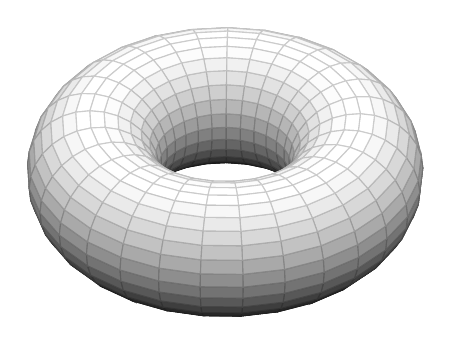
\begin{tikzpicture}
    \begin{axis}[hide axis,view={60}{60}]
       \addplot3[
	surf,
%colormap name=viridis,
       colormap={bw}{gray(0 cm)=(0);gray(1 cm)=(1)},
       samples=30,
       domain=0:360,y domain=0:360,
       z buffer=sort]
       ({(2+cos(x))*cos(y)}, 
        {(2+cos(x))*sin(y)}, 
        {0.2*sin(x)});
    \end{axis}
\end{tikzpicture}%
\caption*{(ب)}
\end{subfigure}%
\caption{اندرسہ}
\label{شکل_خطی_تکمل_اندرسہ}
\end{figure}

مساوات \حوالہ{مساوات_خطی_تکمل_پہلی_بنیادی_صورت_الف} سے
\begin{align*}
E=(a+b\cos v)^2,\quad F=0,\quad G=b^2
\end{align*}
لکھا جا سکتا ہے لہٰذا
\begin{align*}
\abs{\bM{r}_u\times \bM{r}_v}^2=EG-F^2=b^2(a+b\cos v)^2
\end{align*}
ہو گا جس سے اندرسہ کی سطح کا رقبہ درج ذیل حاصل ہوتا ہے۔
\begin{align*}
A=\int_{0}^{2\pi}\int_0^{2\pi}b(a+b\cos v)\dif u\dif v=4ab\pi^2
\end{align*}
\انتہا{مثال}
%====================

فرض کریں کہ کسی سطح کی مساوات درج ذیل ہے۔
\begin{align}
z=g(x,y)
\end{align}
اس میں \عددی{x=u} اور \عددی{y=v} پر کرتے ہوئے مقدار معلوم روپ
\begin{align}
\bM{r}(u,v)=u\bM{i}+v\bM{j}+g(u,v)\bM{k}
\end{align}
میں لکھا جا سکتا ہے جس کے \عددی{u} اور \عددی{v} کے ساتھ جزوی تفرق درج ذیل ہیں۔
\begin{align}\label{مساوات_خطی_تکمل_جزوی_تفرقات_الف}
\bM{r}_u=\bM{i}+g_u\bM{k},\quad \bM{r}_v=\bM{j}+g_v\bM{k}
\end{align}
اس طرح اول بنیادی صورت کے عددی سر
\begin{align*}
E=1+g_u^2,\quad F=g_ug_v,\quad G=1+g_v^2
\end{align*}
ہوں گے لہٰذا
\begin{align*}
\abs{\bM{r}_u\times \bM{r}_v}^2=EG-F^2=1+g_u^2+g_v^2
\end{align*}
ہو گا۔اب چونکہ \عددی{u=x} اور \عددی{v=y} ہیں  لہٰذا رقبہ درج ذیل ہو گا
\begin{align}\label{مساوات_خطی_تکمل_صریح_تفاعل_رقبہ_الف}
A=\iint\limits_{\overline{S}} \sqrt{1+\big(\frac{\partial g}{\partial x}\big)^2+\big(\frac{\partial g}{\partial y}\big)^2}\,\dif x\dif y
\end{align}
جہاں سطح \عددی{S} کا \عددی{xy} مستوی پر عمودی سایہ \عددی{\overline{S}} ہے۔اس سے ظاہر ہے کہ
\begin{align}\label{مساوات_خطی_تکمل_صریح_تفاعل_رقبہ_ب}
\dif A=\sqrt{1+\big(\frac{\partial g}{\partial x}\big)^2+\big(\frac{\partial g}{\partial y}\big)^2}\,\dif x\dif y
\end{align}
ہو گا۔بعد میں استعمال کی خاطر ہم ثابت کرتے ہیں کہ اس کو
\begin{align}\label{مساوات_خطی_تکمل_صریح_تفاعل_رقبہ_پ}
\dif A=\sec \delta \, \dif x\dif y
\end{align}
لکھا جا سکتا ہے جہاں \عددی{S} کی (غیر سمتی) عمود اور \عددی{z} محور کے درمیان زاویہ حادہ \عددی{\delta} ہے۔ شکل \حوالہ{شکل_مساوات_خطی_تکمل_صریح_تفاعل_رقبہ_پ} سے اس کی جیومیٹریائی وجہ ظاہر ہے جہاں چھوٹا رقبہ \عددی{\Delta A} کا \عددی{xy} مستوی پر عمودی عکس
 \عددی{\Delta  A\cos \delta} ہو گا جو \عددی{\Delta x\Delta y} کے برابر ہو گا جس کو \عددی{\overline{\Delta A}} لکھا جاتا ہے۔یوں درج ذیل ہو گا۔
\begin{align*}
\Delta A=\overline{\Delta A} \sec \delta=\sec \delta \, \Delta x\Delta y
\end{align*} 
%
\begin{figure}
\centering
\begin{tikzpicture}
\draw(0,0)--(-0.75,-0.75)node[left]{$x$};
\draw(0,0)--(3,0)node[right]{$y$};
\draw(0,0)node[ocirc]{}--(0,1)node[left]{$z$};
%surface
\draw(0.8,0.5)coordinate(kA) to [out=30,in=-170] ++(1,0.5)coordinate(kB);
\draw(kA) to [out=70,in=-150]++(0.5,0.5)coordinate(kD);
\draw(kD) to [out=30,in=-170]++(1,0.5)coordinate(kC);
\draw(kB) to [out=70,in=-150](kC);
%
\draw($(kA)!0.5!(kC)$)--++(130:1)node[left]{عمود};
\draw[dashed]($(kA)!0.5!(kC)$)coordinate(kE)--++(0,1);
\draw([shift={(90:0.5)}]kE) arc (90:130:0.5);
\draw(kE)++(90+20:0.8)node{$\delta$};
%
\draw[dashed](kA)--++(0,-1.5)coordinate(kAA);
\draw[dashed](kB)--++(0,-2)coordinate(kBB);
\draw[dashed](kC)--++(0,-2)coordinate(kCC);
\draw[dashed](kD)--++(0,-1.5)coordinate(kDD);
\draw(kAA)--(kBB)--(kCC)--(kDD)--(kAA);
\draw($(kAA)!0.5!(kBB)$)node[below]{$\Delta y$};
\draw($(kCC)!0.5!(kBB)$)node[right]{$\Delta x$};
%
\draw[stealth-]($(kA)!0.7!(kC)$) to [out=90,in=180]++(0.5,0.5)node[right]{$\Delta A$};
\end{tikzpicture}
\caption{مساوات \حوالہ{مساوات_خطی_تکمل_صریح_تفاعل_رقبہ_پ} کا ثبوت}
\label{شکل_مساوات_خطی_تکمل_صریح_تفاعل_رقبہ_پ}
\end{figure}

مساوات \حوالہ{مساوات_خطی_تکمل_صریح_تفاعل_رقبہ_پ} کی اب تحلیلی ثبوت پیش کرتے ہیں۔فرض کریں کہ \عددی{\bM{a}=\bM{r}_u\times \bM{r}_v} ہے۔یہ جانتے ہوئے کہ \عددی{u=x} اور \عددی{v=y} ہیں اور مساوات \حوالہ{مساوات_خطی_تکمل_جزوی_تفرقات_الف} کو استعمال کرتے ہوئے سمتی ضرب کی تعریف سے
\begin{align*}
\bM{a}=\frac{\partial \bM{r}}{\partial x}\times \frac{\partial \bM{r}}{\partial y}=-\frac{\partial g}{\partial x}\bM{i}-\frac{\partial g}{\partial y}\bM{j}+\bM{k},\quad \abs{\bM{a}}=\sqrt{1+\big(\frac{\partial g}{\partial x}\big)^2+\big(\frac{\partial g}{\partial y}\big)^2}
\end{align*}  
لکھا جا سکتا ہے لہٰذا \عددی{\bM{a}\cdot \bM{k}=1} ہو گا۔اب اندرونی ضرب کی تعریف سے  \عددی{\bM{a}\cdot \bM{k}=\abs{\bM{a}}\cos \delta^*} ہو گا جہاں \عددی{\bM{a}} اور مثبت \عددی{z} محور کے درمیان زاویہ  \عددی{\delta^*} ہے۔ان کو  ملا کر \عددی{\abs{\bM{a}}\cos \delta^*=1} ملتا ہے جس سے  \عددی{\cos \delta^* >0} اخذ ہوتا ہے لہٰذا \عددی{\delta^* < \tfrac{\pi}{2}} ہو گا یعنی \عددی{\delta^*} زاویہ حادہ ہے اور یوں \عددی{\delta^*=\delta} ہے۔اس طرح درج ذیل لکھا جا سکتا ہے جس سے مساوات \حوالہ{مساوات_خطی_تکمل_صریح_تفاعل_رقبہ_پ} کا ثبوت مکمل ہوتا ہے۔
\begin{align*}
\abs{\bM{a}}\cos \delta=1,\quad \implies \quad \sec \delta=\abs{\bM{a}}\quad \quad \big(\delta < \frac{\pi}{2}\big) 
\end{align*}

%=================================
\حصہء{سوالات}
%==========================
\ابتدا{سوال}\شناخت{سوال_خطی_تکمل_مماسی_سطح_عمومی_مساوات}\quad ثابت کریں کہ نقطہ \عددی{N} پر سطح \عددی{S:\bM{r}(u,v)} کی مماسی سطح کو 
\begin{align}\label{مساوات_سوال_خطی_تکمل_مماسی_سطح_عمومی}
\bM{r}^*(p,q)=\bM{r}+p\bM{r}_u+q\bM{r}_v
\end{align}
لکھا جا سکتا ہے جہاں \عددی{\bM{r},\bM{r}_u,\bM{r}_v} کی قیمتیں نقطہ \عددی{N} کے لحاظ سے ہیں۔مزید ثابت کریں کہ اس کو درج ذیل غیر سمتی سہ ضرب لکھا جا سکتا ہے۔
\begin{align*}
(\bM{r}^*-\bM{r}\quad \bM{r}_u\quad \bM{r}_v)=0
\end{align*}
جواب:\quad شکل \حوالہ{شکل_خطی_تکمل_مماسی_سطح_اور_عمود} میں مماسی سطح پر نقطہ \عددی{N} سے کسی بھی نقطے تک سمتیہ کو خطی طور غیر تابع سمتیات \عددی{\bM{r}_u} اور \عددی{\bM{r}_v} سے ظاہر کیا جا سکتا ہے۔یوں شکل \حوالہ{شکل_سوال_خطی_تکمل_مماسی_سطح_عمومی_الف} میں  تعین گر سمتیہ \عددی{\bM{r}^*} کو  مساوات \حوالہ{مساوات_سوال_خطی_تکمل_مماسی_سطح_عمومی} کی صورت میں لکھا جا سکتا ہے۔
\انتہا{سوال}
%========================
\ابتدا{سوال}\شناخت{سوال_خطی_تکمل_مماسی_سطح_عمومی_الف}\quad سطح \عددی{f(x,y,z)=0} کا نقطہ \عددی{N_0} پر  مماسی سطح کی مساوات دریافت کریں۔اس نقطے پر اس کا اکائی عمودی سمتیہ بھی دریافت کریں۔\\
جوابات:\quad اگر نقطہ \عددی{N_0} کا تعین گر سمتیہ  \عددی{\bM{r}}  جبکہ مماسی سطح پر عمومی نقطے کا تعین گر سمتیہ \عددی{\bM{r}^*} ہو (شکل \حوالہ{شکل_سوال_خطی_تکمل_مماسی_سطح_عمومی_الف}) تب سمتیہ \عددی{\bM{r}^*-\bM{r}} نقطہ \عددی{N_0} پر سطح کا مماس ہو گا۔چونکہ \عددی{\nabla f} سطح کا عمود ہے لہٰذا مماسی سطح کی مساوات \عددی{(\bM{r}^*-\bM{r})\cdot \nabla f=0} ہو گی۔اکائی عمودی سمتیہ \عددی{\bM{n}=\tfrac{\nabla f}{\abs{\nabla f}}} ہو گا۔ 
\begin{figure}
\centering
\begin{tikzpicture}
\pgfmathsetmacro{\ang}{atan(2/3)}
\pgfmathsetmacro{\len}{sqrt(9+4)}
%\draw(0,0) grid (4,2);
%\draw[gray,thin,step=0.1] (0,0) grid (4,2);
%
\draw[name path=kcurve](0.25,1) to [out=30,in=180](1,1.5) to [out=0,in=180](3.5,0.75) to [out=0,in=-90](4,1)to [out=90,in=0] (2,2) to [out=180,in=45](1,1.8) --(0.25,1);
\draw(0.25,1) to [out=-135,in=90](0,0.8) to [out=-90,in=180](0.25,0.7) to [out=0,in=-135] (2,1.25);
\draw(0.75,1)node[]{$S$};
%
\path[](3.5,1.2)coordinate(kA)--++(0.8,0.4)coordinate(kB)--++(-1.6,1)coordinate(kC)--++(-0.8,-0.4)coordinate(kD)--(3.5,1.2);
\path(kD)--++(0,-0.05)coordinate(kE)--++(1.6,-1)coordinate(kF)--++(0.8,0.4)coordinate(kG)--++(0,0.05);
\draw[fill=white](kB)--(kC)--(kD)--(kE)--(kF)--(kG)--(kB);
\draw(kD)--(kA)--(kB);
\draw(kA)--(kF);
%
\path[name path=pointA](0,0)--++(\ang:\len);
\path[name path=pointB](0,0)--++(\ang-10:\len+0.5)coordinate(kB);
\draw[name intersections={of=pointA and kcurve}] (0,0)--(intersection-1)node[pos=0.4,shift={(-0.3,0)}]{$\bM{r}$};
\draw[dashed,-latex](intersection-1)--(3,2)coordinate(kTA)node[shift={(-0.3,0.2)}]{$N_0$};
\draw[name intersections={of=pointB and kcurve}] (0,0)--(intersection-1)node[pos=0.8,below]{$\bM{r}^*$};
\draw[dashed,-latex](intersection-1)--(kB);
\draw[-latex](kTA)node[ocirc]{}--(kB)coordinate[pos=0.5](kM);
\draw[stealth-] (kM) to [out=45,in=180]++(0.5,0.5)node[right]{$\bM{r}-\bM{r}^*$};
%
\draw(0,0)--++(-0.5,-0.5)node[left]{$x$};
\draw(0,0)--++(1,0)node[below]{$y$};
\draw(0,0)--++(0,0.5)node[left]{$z$};
\end{tikzpicture}
\caption{مماسی سطح کی مساوات (سوال \حوالہ{سوال_خطی_تکمل_مماسی_سطح_عمومی_مساوات} اور سوال \حوالہ{سوال_خطی_تکمل_مماسی_سطح_عمومی_الف})}
\label{شکل_سوال_خطی_تکمل_مماسی_سطح_عمومی_الف}
\end{figure}
\انتہا{سوال}
%======================
\ابتدا{سوال}\quad سطح \عددی{z=g(x,y)} کا نقطہ \عددی{N_0} پر مماسی سطح کی مساوات دریافت کریں۔ مزید اس نقطے پر اکائی عمودی سمتیہ بھی دریافت کریں۔\\
جوابات:\quad
$xg_x+yg_y-z=x_0g_x+y_0g_y-g(x_0,y_0),\quad \bM{n}=\tfrac{g_x\bM{i}+g_y\bM{j}-\bM{k}}{\sqrt{g_x^2+g_y^2+1}}$
\انتہا{سوال}
%==========================
\ابتدا{سوال}\quad اگر سطح \عددی{S:\,\bM{r}(u,v)} کا اکائی عمودی سمتیہ  \عددی{\bM{n}} ہو  (مساوات \حوالہ{مساوات_خطی_تکمل__سطح_اکائی_عمودی_سمتیہ}) تب \عددی{u=-\tilde{u}}، \عددی{v=\tilde{v}} پر کرتے ہوئے ثابت کریں کہ  \عددی{\bM{r}^*(\tilde{u},\tilde{v})} کا اکائی عمودی سمتیہ \عددی{-\bM{n}} ہو گا۔ \\
جواب:\quad مساوات \حوالہ{مساوات_خطی_تکمل__سطح_اکائی_عمودی_سمتیہ} کے تحت \عددی{\bM{n}=\tfrac{\bM{r}_u\times \bM{r}_v}{\abs{\bM{r}_u\times \bM{r}_v}}} ہے۔ \عددی{\bM{r}^*(\tilde{u},\tilde{v})}  استعمال کرتے ہوئے 
\begin{align*}
\bM{r}_u^*(\tilde{u},\tilde{v})=\frac{\partial \bM{r}}{\partial \tilde{u}}\frac{\partial \tilde{u}}{\partial u}+\frac{\partial \bM{r}}{\partial \tilde{v}}\frac{\partial \tilde{v}}{\partial u}=-\bM{r}_u,\quad
\bM{r}_v^*(\tilde{u},\tilde{v})=\frac{\partial \bM{r}}{\partial \tilde{u}}\frac{\partial \tilde{u}}{\partial v}+\frac{\partial \bM{r}}{\partial \tilde{v}}\frac{\partial \tilde{v}}{\partial v}=\bM{r}_v
\end{align*}
سے اکائی عمودی سمتیہ \عددی{-\tfrac{\bM{r}_u\times \bM{r}_v}{\abs{\bM{r}_u\times \bM{r}_v}}} حاصل ہوتا ہے جو \عددی{-\bM{n}}  کے برابر ہے۔
\انتہا{سوال}
%=========================
سوال \حوالہ{سوال_خطی_تکمل_مماسی_سطح_الف} تا سوال \حوالہ{سوال_خطی_تکمل_مماسی_سطح_ب} میں نقطہ \عددی{N_0:(x_0,y_0,z_0)} پر سطح  کی مماسی سطح کی مساوات حاصل کریں۔

%====================
\ابتدا{سوال}\شناخت{سوال_خطی_تکمل_مماسی_سطح_الف}\quad
$z=xy,\quad N_0:(3,2,6)$\\
جواب:\quad \عددی{f=xy-z=0} لکھتے ہوئے \عددی{\nabla f=y\bM{i}+x\bM{j}-\bM{k}} ملتا ہے جس کی \عددی{N_0} پر قیمت 
\عددی{\nabla f_N=2\bM{i}+3\bM{j}-\bM{k}} ہے۔ہم \عددی{N_0} کا تعین گر سمتیہ \عددی{\bM{r}=3\bM{i}+2\bM{j}+6\bM{k}} اور مماسی سطح پر عمومی نقطے کا تعین گر سمتیہ \عددی{\bM{r}^*=x\bM{i}+y\bM{j}+z\bM{k}}  لکھتے ہیں۔یوں \عددی{\bM{r}-\bM{r}^*=(x-3)\bM{i}+(y-2)\bM{j}+(z-6)\bM{k}} ہو گا۔ اس طرح \عددی{(\bM{r}-\bM{r}^*)\cdot \nabla f_N=0} سے  مماسی سطح کی مساوات \عددی{2x+3y-z=6}  حاصل ہوتی ہے۔
\انتہا{سوال}
%=====================
\ابتدا{سوال}\quad
$x^2+y^2+z^2=25,\quad N_0:(\sqrt{2},\sqrt{2},3)$\\
جواب:\quad 
$\sqrt{2}x+\sqrt{2}y+3z=13$
\انتہا{سوال}
%=====================
\ابتدا{سوال}\quad
$y=x^2,\quad N_0:(2,4,3)$\\
جواب:\quad 
$4x-y=4$
\انتہا{سوال}
%=====================
\ابتدا{سوال}\quad
$x^2+y^2=8,\quad N_0:(2,2,3)$\\
جواب:\quad 
$x+y=4$
\انتہا{سوال}
%=====================
\ابتدا{سوال}\quad
$z=x^2+y^2,\quad N_0:(2,3,13)$\\
جواب:\quad 
$4x+6y-z=13$
\انتہا{سوال}
%=====================
\ابتدا{سوال}\شناخت{سوال_خطی_تکمل_مماسی_سطح_ب}\quad
$2x^2+y^2+3z^2=9,\quad N_0:(1,2,1)$\\
جواب:\quad 
$2x+2y-3z=3$
\انتہا{سوال}
%=====================
سوال \حوالہ{سوال_خطی_تکمل_اول_بنیادی_صورت_الف} تا سوال \حوالہ{سوال_خطی_تکمل_اول_بنیادی_صورت_ب} میں اول بنیادی صورت دریافت کریں۔

%===============
\ابتدا{سوال}\شناخت{سوال_خطی_تکمل_اول_بنیادی_صورت_الف}\quad 
$\bM{r}=u\bM{i}+v\bM{j}$\\
جواب:\quad
$\dif u^2+\dif v^2$
\انتہا{سوال}
%===================
\ابتدا{سوال}\quad 
$\bM{r}=u\bM{i}+v\bM{j}+uv\bM{k}$\\
جواب:\quad
$(v^2+1)\dif u^2+2uv\dif u\dif v+(u^2+1)\dif v^2$
\انتہا{سوال}
%===================
\ابتدا{سوال}\quad  کرہ \quad
$\bM{r}=a\cos v \cos u\bM{i}+a\cos v \sin u\bM{j}+a\sin v\bM{k}$\\
جواب:\quad
$a^2\cos^2 v\dif u^2+a^2\dif v^2$
\انتہا{سوال}
%===================
\ابتدا{سوال}\quad  اندرسہ\quad
$\bM{r}=(a+b\cos v) \cos u\bM{i}+(a+b\cos v) \sin u\bM{j}+b\sin v\bM{k},\quad (a>b>0)$\\
جواب:\quad
$(a^2+2ab\cos v+b^2\cos^2 v)\dif u^2+b^2\dif v^2$
\انتہا{سوال}
%===================
\ابتدا{سوال}\quad 
$\bM{r}=u\bM{i}+v\bM{j}+v^2\bM{k}$\\
جواب:\quad
$\dif u^2+(1+4v^2)\dif v^2$
\انتہا{سوال}
%===================
\ابتدا{سوال}\شناخت{سوال_خطی_تکمل_اول_بنیادی_صورت_ب}\quad  بیلن \quad
$\bM{r}=a\cos u\bM{i}+a\sin u\bM{j}+v\bM{k}$\\
جواب:\quad
$a^2\dif u^2+\dif v^2$
\انتہا{سوال}
%===================
\ابتدا{سوال}\quad ثابت کریں کہ سطح \عددی{\bM{r}=\bM{r}(u,v)} پر محددی منحنیات \عددی{u=c_1} اور \عددی{v=c_2} صرف اور صرف اس صورت ایک دوسرے کو زاویہ قائمہ پر قطع کرتی ہیں جب \عددی{F=\bM{r}_u\cdot \bM{r}_v=0} ہو۔  یہاں \عددی{c_1} اور \عددی{c_2} مستقل ہیں۔\\
جواب:\quad \عددی{\bM{r}_u} اور \عددی{\bM{r}_v} ان منحنیات کو مماسی ہیں۔یوں اندرونی ضرب کی تعریف  سے ثبوت مکمل ہوتا ہے۔
\انتہا{سوال}
%=================
سوال \حوالہ{سوال_خطی_تکمل_رقبہ_الف} تا سوال \حوالہ{سوال_خطی_تکمل_رقبہ_ب} میں دیے گئے سطحوں کا رقبہ مساوات \حوالہ{مساوات_خطی_تکمل_رقبہ_الف} کی مدد سے دریافت کریں۔

%=====================
\ابتدا{سوال}\شناخت{سوال_خطی_تکمل_رقبہ_الف}\quad
$x^2+y^2=a^2,\quad 0\le z\le b$\\
جواب:\quad
$2\pi ab$
\انتہا{سوال}
%=======================
\ابتدا{سوال}\quad کرہ \quad
$\bM{r}=a\cos v \cos u\bM{i}+a\cos v \sin u\bM{j}+a\sin v\bM{k}$\\
جواب:\quad
$4\pi a^2$
\انتہا{سوال}
%=======================
\ابتدا{سوال}\quad 
$z=x^2+y^2,\quad 0\le z\le 1$\\
جواب:\quad
$\tfrac{\pi}{6}(\sqrt{125}-1)$
\انتہا{سوال}
%=======================
\ابتدا{سوال}\شناخت{سوال_خطی_تکمل_رقبہ_ب}\quad 
$z^2=x^2+y^2,\quad -1\le z\le 1$\\
جواب:\quad
$2\sqrt{2}\,\pi$
\انتہا{سوال}
%====================

\حصہ{سطحی تکمل}
دوہرا تکمل (حصہ \حوالہ{حصہ_خطی_تکمل_دوہرا_تکمل}) کی تصور کو وسعت دیتے ہوئے سطحی تکمل کا تصور پیدا ہوتا ہے۔سطحی تکمل کی تعریف عین دوہرا تکمل کی طرز پر ہے۔

فرض کریں کہ \عددی{S} کسی سطح کا محدود حصہ ہے اور تفاعل \عددی{f(x,y,z)} سطح \عددی{S} پر معین اور استمراری ہے۔ہم مکمل بے قاعدگی سے \عددی{S} کو \عددی{S_1}، \نقطے، \عددی{S_n} ٹکڑوں میں تقسیم کرتے ہیں جن کے  رقبے بالترتیب  \عددی{\Delta A_1}، \نقطے، \عددی{\Delta A_n} ہیں۔ ہم مکمل بے قاعدگی سے ہر \عددی{S_k} میں کوئی نقطہ \عددی{N_k}  منتخب کرتے ہیں جس کے محدد \عددی{x_k}، \عددی{y_k}، \عددی{z_k} ہوں گے۔اب ہم درج ذیل مجموعہ حاصل کرتے ہیں۔
\begin{align}\label{مساوات_خطی_تکمل_سطحی_تکمل_الف}
J_n=\sum_{k=1}^{n}f(x_k,y_k,z_k)\Delta A_k
\end{align}
ہم ایسے مجموعے \عددی{n=1,2,\cdots} کے لئے مکمل بے قاعدگی کے ساتھ یوں حاصل کرتے ہیں کہ \عددی{n} کی قیمت لامتناہی کے قریب کرنے سے سب سے بڑا حصہ \عددی{S_k} نقطہ مانند ہوتا ہو۔ یوں حاصل اعداد \عددی{J_1}، \عددی{J_2}، \نقطے کا ایک حد پایا جاتا ہے جس کی قیمت پر نا تو حصوں کی انتخاب اور نا ہی ہر حصے میں نقطہ کی انتخاب کا کوئی اثر پایا جاتا ہے (مثال \حوالہ{مثال_سمتی_تکمل_رقبہ_اور_تکمل} کی طرح)۔اس حد کو \عددی{S} پر تفاعل \عددی{f(x,y,z)} کی \اصطلاح{سطحی تکمل}\فرہنگ{سطحی!تکمل}\فرہنگ{تکمل!سطحی}\حاشیہب{surface integral}\فرہنگ{surface integral} کہتے ہیں جس کو درج ذیل سے ظاہر کیا جاتا ہے۔
\begin{align}\label{مساوات_خطی_تکمل_سطحی_تکمل_ب}
\iint\limits_S f(x,y,z)\dif A
\end{align}
سطحی تکمل (مساوات \حوالہ{مساوات_خطی_تکمل_سطحی_تکمل_ب}) کی قیمت حاصل کرنے کی خاطر آئیں اس کو دوہرا تکمل میں تبدیل کرتے ہیں۔

اگر \عددی{S} کی مقدار معلوم روپ \عددی{\bM{r}(u,v)} ہو تب \عددی{\dif A=\abs{\bM{r}_u\times \bM{r}_v}\dif u\dif v=\sqrt{EG-F^2}\,\dif u\dif v} ہو گا (مساوات \حوالہ{مساوات_خطی_تکمل_رقبہ_ب} اور مساوات \حوالہ{مساوات_خطی_تکمل_رقبہ_ٹ}) لہٰذا
\begin{gather}
\begin{aligned}\label{مساوات_خطی_تکمل_سطحی_تکمل_بطور_دوہرا_الف}
\iint\limits_S f(x,y,z)\dif A&=\iint\limits_R f[x(u,v),y(u,v),z(u,v)] \abs{\bM{r}_u\times \bM{r}_v}\dif u\dif v\\
&=\iint\limits_R f[x(u,v),y(u,v),z(u,v)] \sqrt{EG-F^2}\dif u\dif v 
\end{aligned}
\end{gather}
لکھا جا سکتا ہے جہاں \عددی{uv} سطح میں \عددی{R} سطح \عددی{S} کا مطابقتی خطہ ہے۔ 

اسی طرح اگر \عددی{S} کو \عددی{z=g(x,y)} سے ظاہر کیا گیا ہو تب مساوات \حوالہ{مساوات_خطی_تکمل_صریح_تفاعل_رقبہ_ب} کی مدد سے درج ذیل ہو گا۔
\begin{align}\label{مساوات_خطی_تکمل_سطحی_تکمل_بطور_دوہرا_ب}
\iint\limits_S f(x,y,z)\dif A=\iint\limits_{\overline{S}} f[x,y,g(x,y)]\sqrt{1+\big(\frac{\partial g}{\partial x}\big)^2+\big(\frac{\partial g}{\partial y}\big)^2}\,\dif x\dif y
\end{align}

%====================
\ابتدا{مثال}\quad جمودی معیار اثر\\
کروی یکساں خاصیت کی جھلی \عددی{S:\, x^2+y^2+z^2=a^2} جس کی کمیت \عددی{M} ہے کا \عددی{z} محور کے لحاظ سے جمودی معیار اثر دریافت کریں۔

اگر کمیت سطح \عددی{S} پر یوں پھیلا ہو کہ کمیت کی سطحی کثافت \عددی{\mu(x,y,z)} ہو تب کسی محور \عددی{L} کے لحاظ سے جمودی معیار اثر
\begin{align}
I=\iint\limits_S \mu D^2\dif A
\end{align}
ہو گا جہاں \عددی{L}  سے نقطہ \عددی{(x,y,z)} تک فاصلہ \عددی{D(x,y,z)} ہے۔

چونکہ موجودہ مثال میں جھلی یکساں خاصیت رکھتی ہے لہٰذا \عددی{\mu} ایک مستقل ہو گا۔ کروی جھلی کا رقبہ \عددی{A=4\pi a^2} ہے لہٰذا
\begin{align*}
\mu=\frac{M}{A}=\frac{M}{4\pi a^2}
\end{align*}
ہو گا۔کرہ کو مساوات \حوالہ{مساوات_خطی_تکمل_خطوط_عرض_بلد_طول_بلد} سے ظاہر کرتے ہوئے مساوات \حوالہ{مساوات_خطی_تکمل_پہلی_بنیادی_صورت_الف} سے
\begin{align*}
E=a^2\cos^2 v,\quad F=0,\quad G=a^2
\end{align*}
حاصل ہوتا ہے لہٰذا
\begin{align*}
\dif A=\abs{\bM{r}_u\times \bM{r}_v}\dif u\dif v=\sqrt{EG-F^2}\,\dif u\dif v=a^2\cos v\,\dif u\dif v
\end{align*}
ہو گا۔ مزید \عددی{z} محور سے کسی نقطہ \عددی{(x,y,z)} کا فاصلہ \عددی{D=\sqrt{x^2+y^2}=a\cos v} ہو گا۔یوں درج ذیل ملتا ہے۔
\begin{align*}
I=\iint\limits_S \mu D^2 \dif A=\frac{M}{4\pi a^2}\int\limits_{-\frac{\pi}{2}}^{\frac{\pi}{2}} \int\limits_{0}^{2\pi} a^4\cos^3 v \dif u\dif v=\frac{2Ma^2}{3}
\end{align*}
\انتہا{مثال}
%=========================

کئی عملی سطحی تکمل میں سطح کی سمت بندی اہمیت رکھتی ہے لہٰذا ہموار سطح (حصہ \حوالہ{حصہ_خطی_تکمل_سطحیں}) سے شروع کرتے ہوئے  سطح کی سمت بندی پر غور کرتے ہیں۔

فرض کریں کہ \عددی{S} ایک ہموار سطح ہے جس پر \عددی{N} کوئی نقطہ ہے۔ہم \عددی{N} پر \عددی{S} کا اکائی عمودی سمتیہ \عددی{\bM{n}} منتخب کر سکتے ہیں۔یوں \عددی{\bM{n}} کی سمت \عددی{N} پر \عددی{S} کی مثبت عمودی سمت  ہو گی۔ظاہر ہے کہ \عددی{\bM{n}} کو دو ہی  طریقوں سے (آپس میں الٹ رخ) چنا جا سکتا ہے۔  

ایک ہموار سطح اس صورت \اصطلاح{قابل سمت بند}\فرہنگ{سمت بند!قابل}\حاشیہب{orientable}\فرہنگ{orientable} کہلاتی ہے جب اس سطح پر کسی نقطہ \عددی{N_0} پر دی  گئی مثبت سمت کو پوری سطح پر یکتا اور استمراری طور پر جاری رکھنا ممکن ہو۔

یوں سطح \عددی{S} اس صورت قابل سمت بند ہو گی جب اس پر نقطہ \عددی{N_0} سے گزرتی کوئی ایسی سطح \عددی{C} نہ پائی جاتی ہو جس پر منتخب کردہ مثبت سمت کو \عددی{C} پر مسلسل ایک جگہ سے دوسری جگہ منتقل کرنے کے بعد واپس \عددی{N_0} لانے سے سمت الٹ ہوتی ہو۔    

ہموار سطح کا (حسب ضرورت) چھوٹا حصہ ہر صورت قابل سمت بند ہوتا ہے۔البتہ وسیع سطح کے لئے ایسا نہیں کہا جا سکتا ہے۔غیر قابل سمت بند سطحیں پائی جاتی ہیں جن کی مشہور مثال \اصطلاح{موبیوس پٹی}\فرہنگ{موبیوس پٹی}\حاشیہب{Mobius strip}\فرہنگ{Mobius strip} کو شکل \حوالہ{شکل_خطی_تکمل_موبیوس_پٹی} میں دکھایا گیا ہے۔اس شکل میں نقطہ \عددی{N_0} پر عمودی سمتیہ کو نقطہ دار لکیر پر  حرکت دے کر  واپس \عددی{N_0} پہنچانے سے  عمودی سمتیہ کا رخ الٹ ہو جائے گا۔کاغذ کی لمبی مستطیل پٹی کو بل دے کر چھوٹے اطراف کو آپس میں یوں جوڑنے سے کہ \عددی{A} اور \عددی{A} آپس میں ملیں اور \عددی{B} اور \عددی{B} آپس میں ملیں، موبیوس پٹی\حاشیہد{جرمن ریاضی دان اگست فرڈینانڈ موبیوس [1790-1868]} بنائی جا سکتی ہے۔
\begin{figure}
\centering
\begin{subfigure}{0.5\textwidth}
\centering
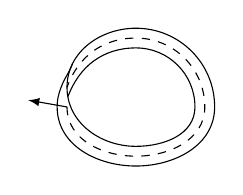
\begin{tikzpicture}
%
\draw  (0,0) to [out=-90,in=180](1,-0.75) to [out=0,in=-90](2,0) to [out=90,in=0](1,1) to [out=180,in=90](0.125,0.25) to [out=-90,in=180](1,-0.5) to [out=0,in=-90](1.75,0) to [out=90,in=0](1,0.75) to [out=180,in=70](0.135,0.125);
\draw(0,0) to [out=90,in=-110]++(0.05,0.25) to [out=70,in=-110](0.195,0.55);
\draw[-latex](0.125,0)--++(170:0.5);
%
\draw[dashed]  (0.125,0) to [out=-90,in=180](1,-0.625) to [out=0,in=-90](1.875,0) to [out=90,in=0](1,0.875) to [out=180,in=70](0.125,0.25);
\end{tikzpicture}%
\caption{موبیوس پٹی}
\label{شکل_خطی_تکمل_موبیوس_پٹی}
\end{subfigure}%
\begin{subfigure}{0.5\textwidth}
\centering
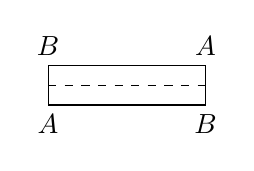
\begin{tikzpicture}
\draw(0,0)node[below]{$A$} --++(2,0)node[below]{$B$}--++(0,0.5)node[above]{$A$}--++(-2,0)node[above]{$B$}--++(0,-0.5);
\draw[dashed](0,0.25)--++(2,0);
\end{tikzpicture}
\end{subfigure}%
\end{figure}
اگر \عددی{S} قابل سمت بند ہو تب ہم \عددی{\bM{n}} کی دو میں سے ایک ممکنہ رخ کو مثبت سمت کہتے ہوئے \عددی{S} کو سمت بند بنا سکتے ہیں۔

اگر \عددی{S} کی سرحد \عددی{C} سادہ بند منحنی ہو تب ہم \عددی{\bM{n}} کے لحاظ سے  \عددی{C} کو سمت بند بنا سکتے ہیں۔یہ عمل شکل \حوالہ{شکل_خطی_تکمل_سطح_سمت_بندی}-الف میں دونوں ممکنہ عمودی سمتیات کے لحاظ سے دکھایا گیا ہے۔ ہم اب سمت بندی کی تصور کو وسعت دیتے ہوئے اس کو ٹکڑوں میں ہموار سطحوں کے لئے بیان کرتے ہیں۔
\begin{figure}
\centering
\begin{subfigure}{0.5\textwidth}
\centering
\begin{tikzpicture}
\draw[-stealth](0,0)node[left]{$C$} to [out=-90,in=180](2,-1) to [out=0,in=-90] (3,0) to [out=90,in=0](1.5,0.5) to [out=180,in=90] (0,0);
\draw[-latex](1.5,-0.25)node[ocirc]{}--++(80:1.5)node[left]{$\bM{n}$};
\draw(2,0)node[]{$S$};
\begin{scope}[shift={(4cm,0)}]
\draw[-stealth,name path=kk](0,0)node[left]{$C$} to [out=-90,in=180](2,-1) to [out=0,in=-90] (3,0) to [out=90,in=0](1.5,0.5) to [out=180,in=90] (0,0);
\path[name path=kdir](1.5,-0.25)--++(-100:1.5)coordinate(kdirT);
\draw[dashed,name intersections={of=kk and kdir}](1.5,-0.25)node[ocirc,solid]{}--(intersection-1);
\draw[-latex](intersection-1)--(kdirT)node[left]{$\bM{n}$};
\draw(2,0)node[]{$S$};
\end{scope}
\end{tikzpicture}
\caption*{(الف) ہموار سطح}
\end{subfigure}
\begin{subfigure}{0.5\textwidth}
\centering
\begin{tikzpicture}
\draw (0,0) to [out=50,in=-150]++(1,0.6) to [out=-40,in=130]++(1,-0.4) to [out=-130,in=50]++(-1,-0.6)coordinate(kA)--(0,0);
\draw(0,0) to [out=-170,in=45]++(-1,-0.4) to [out=-40,in=130]++(1,-0.4) to [out=50,in=-170]++(1,0.4);
\draw[-latex](-0.25,-0.25)node[ocirc]{}--++(110:0.75)node[left]{$\bM{n}$};
\draw[-latex](1,0.25)node[ocirc]{}--++(140:0.75)node[above]{$\bM{n}$};
%
\draw[stealth-] (-0.8,-0.4) to [out=-170,in=0]++(-0.5,-0.5)node[left]{$S_1$};
\draw[stealth-] (1.5,0.2) to [out=-30,in=180]++(0.5,-0.5)node[right]{$S_2$};
%
\draw[-latex] (kA)++(-0.25,0)--++(155:0.4);
\draw[latex-] (kA)++(0,0.125)--++(160:0.4)coordinate(kC);
\draw(kC)++(160:0.4)++(0.3,0)node{$C^*$};
\end{tikzpicture}
\caption*{(ب) ٹکڑوں میں ہموار سطح}
\end{subfigure}%
\caption{سطح کی سمت بندی}
\label{شکل_خطی_تکمل_سطح_سمت_بندی}
\end{figure}
ٹکڑوں میں ہموار سطح \عددی{S} اس صورت قابل سمت بند ہو گی جب ایسا ممکن ہو کہ ہر دو ٹکڑوں \عددی{S_1} اور \عددی{S_2} کے مابین مشترکہ سرحدی منحنی \عددی{C^*} کی مثبت سمت \عددی{S_1}  اور \عددی{S_2} کے لحاظ سے آپس میں الٹ ہوں۔ شکل \حوالہ{شکل_خطی_تکمل_سطح_سمت_بندی}-ب میں ایسا دکھایا گیا ہے۔

فرض کریں کہ \عددی{S}  ٹکڑوں میں قابل سمت بند سطح ہے۔ہم اکائی عمودی سمتیہ \عددی{\bM{n}} چنتے ہوئے \عددی{S} کو سمت بند کرتے ہیں۔ \عددی{\bM{n}} اور مثبت \عددی{x}، \عددی{y}، \عددی{z} محور  کے درمیان زاویوں کو \عددی{\alpha}، \عددی{\beta}، \عددی{\gamma} سے ظاہر کرتے ہوئے
\begin{align}\label{مساوات_خطی_تکمل_اکائی_عمودی_ارکان}
\bM{n}=\cos \alpha \,\bM{i}+\cos \beta \,\bM{j}+\cos \gamma \, \bM{k}
\end{align}
لکھا جا سکتا ہے۔ مزید فرض کریں کہ تفاعل \عددی{u_1(x,y,z)}، \عددی{u_2(x,y,z)}، \عددی{u_3(x,y,z)} سطح  \عددی{S} کے ہر نقطہ  پر  معین اور استمراری ہیں۔ ہمیں عموماً درج ذیل تکملات حل کرنے ہوں گے۔
\begin{align*}
\iint\limits_S u_1\dif y\dif z,\quad \iint\limits_S u_2\dif x\dif z,\quad \iint\limits_S u_3\dif x\dif y
\end{align*}
تکمل کی تعریف کے تحت ان سے مراد درج ذیل ہے (شکل \حوالہ{شکل_مساوات_خطی_تکمل_صریح_تفاعل_رقبہ_پ} سے رجوع کریں)۔
\begin{gather}
\begin{aligned}\label{مساوات_خطی_تکمل_تین_قسم_کے_تکمل_الف}
\iint\limits_S u_1\dif y\dif z&=\iint\limits_S u_1\cos \alpha \dif A\\
\iint\limits_S u_2\dif x\dif z&=\iint\limits_S u_2\cos \beta \dif A\\
\iint\limits_S u_3\dif x\dif y&=\iint\limits_S u_3\cos \gamma \dif A
\end{aligned}
\end{gather}

صاف ظاہر کہ ان تکملات کی قیمت کا دارومدار \عددی{\bM{n}} کی انتخاب یعنی \عددی{S} کی سمت بندی پر ہو گا۔\عددی{S} کی سمت بندی الٹ کرنے سے \عددی{\bM{n}} کے اجزاء \عددی{\cos \alpha}، \عددی{\cos \beta}، \عددی{\cos \gamma} منفی اکائی سے ضرب ہوں گے لہٰذا  تکمل کی قیمت بھی منفی ایک (\عددی{-1}) سے ضرب ہو گی۔

اس طرح کے تین عدد تکملات کو سمتیہ کی استعمال سے نہایت سادہ طرز میں لکھا جا سکتا ہے۔یوں سمتیہ
\begin{align*}
\bM{u}=u_1\bM{i}+u_2\bM{j}+u_3\bM{k}
\end{align*}
متعارف کرتے ہوئے  مساوات \حوالہ{مساوات_خطی_تکمل_تین_قسم_کے_تکمل_الف} سے درج ذیل لکھا جا سکتا ہے۔
\begin{multline}\label{مساوات_خطی_تکمل_عمودی_سمتیہ_اجزاء_استعمال}
\iint\limits_S (u_1\dif y\dif z+u_2\dif x\dif z+u_3\dif x\dif y)\\
=\iint\limits_S (u_1\cos \alpha +u_2\cos \beta+u_3\cos \gamma)\dif A=\iint\limits_S \bM{u}\cdot \bM{n}\dif A
\end{multline}

مساوات \حوالہ{مساوات_خطی_تکمل_تین_قسم_کے_تکمل_الف} کے تکملات حل کرنے کی خاطر انہیں مستوی سطح پر دوہرا تکملات میں تبدیل کیا جاتا ہے۔اس عمل پر غور کرتے ہیں۔

اگر \عددی{S} کو \عددی{z=h(x,y)} سے ظاہر کیا گیا ہو اور اس کی سمت بندی یوں ہو کہ \عددی{\bM{n}} اوپر کی رخ ہو تب \عددی{\gamma} زاویہ حادہ ہو گا لہٰذا مساوات \حوالہ{مساوات_خطی_تکمل_صریح_تفاعل_رقبہ_پ} میں \عددی{\delta=\gamma} ہو گا۔اس طرح مساوات \حوالہ{مساوات_خطی_تکمل_تین_قسم_کے_تکمل_الف} سے 
\begin{align}
\iint\limits_S u_3(x,y,z)\dif x\dif y=+\iint\limits_{\overline{R}} u_3[x,y,h(x,y)]\dif x\dif y
\end{align}
حاصل ہو گا جہاں  \عددی{S} کا قائمہ الزاویہ سایہ \عددی{xy} مستوی پر \عددی{\overline{R}} ہے۔اگر \عددی{\bM{n}} کا رخ نیچے کو ہو تب \عددی{\gamma} زاویہ منفرجہ ہو گا اور ہمیں درج ذیل ملے گا۔
\begin{align}
\iint\limits_S u_3(x,y,z)\dif x\dif y=-\iint\limits_{\overline{R}} u_3[x,y,h(x,y)]\dif x\dif y
\end{align}
مساوات \حوالہ{مساوات_خطی_تکمل_تین_قسم_کے_تکمل_الف} کے باقی دو عدد تکمل کو بھی اسی طرح دوہرا تکمل میں تبدیل کیا جاتا ہے۔

اگر \عددی{S} کو مقدار معلوم روپ
\begin{align*}
\bM{r}(u,v)=x(u,v)\bM{i}+y(u,v)\bM{j}+z(u,v)\bM{k}
\end{align*}
سے ظاہر کیا گیا ہو تب \عددی{S} کی دو ممکنہ عمودی سمتیات درج ذیل ہوں گے۔
\begin{align}\label{مساوات_خطی_تکمل_دو_عدد_سمتیں_الف}
\text{(الف)}\quad \bM{n}=+\frac{\bM{r}_u\times \bM{r}_v}{\abs{\bM{r}_u\times \bM{r}_v}} \quad \quad \text{(ب)}\quad \bM{n}=-\frac{\bM{r}_u\times \bM{r}_v}{\abs{\bM{r}_u\times \bM{r}_v}}
\end{align}
اب مساوات \حوالہ{مساوات_خطی_تکمل_اکائی_عمودی_ارکان} کے دونوں اطراف کا  \عددی{\bM{k}} کے ساتھ اندرونی ضرب لینے  سے \عددی{\cos \gamma=\bM{k}\cdot \bM{n}} ملتا ہے جبکہ مساوات \حوالہ{مساوات_خطی_تکمل_رقبہ_ب} کے تحت \عددی{\dif A=\abs{\bM{r}_u\times \bM{r}_v}\dif u\dif v} ہے لہٰذا درج ذیل لکھا جا سکتا ہے
\begin{align*}
\cos \gamma \dif A&=\bM{k}\cdot \bM{n}\dif A=\mp \bM{k}\cdot (\bM{r}_u\times \bM{r}_v)\dif u\dif v=\mp
\begin{vmatrix}
0&0&1\\
x_u&y_u&z_u\\
x_v&y_v&z_v
\end{vmatrix}
\dif u\dif v\\
&=\mp \frac{\partial (x,y)}{\partial (u,v)}\dif u\dif v
\end{align*}
جہاں آخری قدم پر یعقوبی پایا جاتا ہے (حصہ \حوالہ{حصہ_خطی_تکمل_دوہرا_تکمل})۔ اس طرح مساوات \حوالہ{مساوات_خطی_تکمل_تین_قسم_کے_تکمل_الف} میں
\begin{align}
\iint\limits_S u_3(x,y,z)\dif x\dif y=\mp \iint\limits_R u_3[x(u,v),y(u,v),z(u,v)]\frac{\partial (x,y)}{\partial (u,v)}\dif u\dif v
\end{align}
ہو گا جہاں مثبت علامت  مساوات \حوالہ{مساوات_خطی_تکمل_دو_عدد_سمتیں_الف}-الف  اور منفی علامت  مساوات \حوالہ{مساوات_خطی_تکمل_دو_عدد_سمتیں_الف}-ب کی صورت میں استعمال ہو گا۔یہاں  \عددی{S} کا مطابقتی خطہ \عددی{uv} مستوی میں \عددی{R} ہے۔
%===================

\حصہء{سوالات}

%=====================
سوال \حوالہ{سوال_خطی_تکمل_سطحی_تکمل_الف} تا سوال \حوالہ{سوال_خطی_تکمل_سطحی_تکمل_ب} میں \عددی{S} کو مقدار معلوم روپ میں لکھ کر مساوات \حوالہ{مساوات_خطی_تکمل_سطحی_تکمل_بطور_دوہرا_الف} استعمال کرتے ہوئے \عددی{\iint\limits_S f(x,y,z)\dif A} کی قیمت دریافت کریں۔

%========================
\ابتدا{سوال}\شناخت{سوال_خطی_تکمل_سطحی_تکمل_الف}\quad 
$f=2x-1,\quad S:\,x^2+y^2=1,\quad 0\le z\le 4$\\
جواب:\quad 
$-8\pi$
\انتہا{سوال}
%===========================
\ابتدا{سوال}\quad 
$f=2x,\quad S:\,z=x^2,\quad 0\le x\le 2,\quad -2\le y\le 2$\\
جواب:\quad 
$\tfrac{2}{3}(17\sqrt{17}-1)$
\انتہا{سوال}
%===========================
\ابتدا{سوال}\quad 
$f=xy,\quad S:\,z=xy,\quad -1\le x\le 1,\quad -1\le y\le 1$\\
جواب:\quad 
$0$
\انتہا{سوال}
%===========================
\ابتدا{سوال}\quad 
$f=3x^3\cos y,\quad S:\,z=x^3,\quad 0\le x\le 1,\quad 0\le y\le \frac{\pi}{2}$\\
جواب:\quad 
$\tfrac{10\sqrt{10}-1}{18}$
\انتہا{سوال}
%===========================
\ابتدا{سوال}\quad 
$f=xy,\quad S:\,x^2+y^2=9,\quad -1\le z\le 2$\\
جواب:\quad 
$0$
\انتہا{سوال}
%===========================
\ابتدا{سوال}\quad 
$f=2x-y+z,\quad S:\,x^2+y^2=1,\quad 0\le z\le 1$\\
جواب:\quad 
$\pi$
\انتہا{سوال}
%===========================
\ابتدا{سوال}\quad 
$f=x-2y,\quad S:\,\text{\RL{ربع اول میں $x+y+z=1$}}$\\
جواب:\quad 
$-\tfrac{1}{2\sqrt{3}}$
\انتہا{سوال}
%===========================
\ابتدا{سوال}\شناخت{سوال_خطی_تکمل_سطحی_تکمل_ب}\quad 
$f=2x+3y,\quad S:\,z=y^2,\quad  0\le x\le 1,\quad 0\le y\le 1$\\
جواب:\quad 
$\tfrac{7\sqrt{5}-1\sinh^{-1} 2}{4}$
\انتہا{سوال}
%===========================
\ابتدا{سوال}\quad
فضا میں سطح \عددی{S} کی کثافت کمیت (کمیت فی اکائی رقبہ) \عددی{\sigma(x,y,z)} ہے۔کل کمیت \عددی{M} اور مرکز ثقل \عددی{(\bar{x},\bar{y},\bar{z})} کی درج ذیل کلیات درست ہونے کا جواز پیش کریں۔
\begin{align*}
M=\iint\limits_S \sigma \dif A,\quad \bar{x}=\frac{1}{M}\iint\limits_S x\sigma \dif A,\quad\bar{y}=\frac{1}{M}\iint\limits_S y\sigma \dif A,\quad\bar{z}=\frac{1}{M}\iint\limits_S z\sigma \dif A
\end{align*}
\انتہا{سوال}
%=====================
\ابتدا{سوال}\quad
فضا میں سطح \عددی{S} کی کثافت کمیت (کمیت فی اکائی رقبہ) \عددی{\sigma(x,y,z)} ہے۔درج ذیل کلیات \عددی{x}، \عددی{y}، \عددی{z} محور کے لحاظ سے بالترتیب جمودی معیار اثر \عددی{I_x}، \عددی{I_y}، \عددی{I_z}  دیتے ہیں۔ان کی درست ہونے کا جواز پیش کریں۔
\begin{align*}
I_x=\iint\limits_S (y^2+z^2)\sigma \dif A,\quad I_y=\iint\limits_S (x^2+z^2)\sigma \dif A,\quad I_z=\iint\limits_S (x^2+y^2)\sigma \dif A
\end{align*}
\انتہا{سوال}
%=====================
سوال \حوالہ{سوال_خطی_تکمل_جمودی_معیار_اثر_معلوم_الف} تا سوال \حوالہ{سوال_خطی_تکمل_جمودی_معیار_اثر_معلوم_ت} میں دیے محور کے لحاظ سے جھلی \عددی{S} کی جمودی معیار اثر دریافت کریں۔کثافت \عددی{\sigma=1} ہے۔

%=============================
\ابتدا{سوال}\شناخت{سوال_خطی_تکمل_جمودی_معیار_اثر_معلوم_الف}\quad
$S:x^2+y^2=1,\quad 0\le z \le h,\quad \text{محور}\, z$\\
جواب:\quad
$2\pi h$
\انتہا{سوال}
%======================
\ابتدا{سوال}\quad
$S:x^2+y^2=1,\quad 0\le z \le h,\quad \text{محور}\, z$\\
جواب:\quad
$\tfrac{\sqrt{2}h\sqrt{1-h^2}}{3}(2h^2+1)+\sqrt{2}\sinh^{-1} h$
\انتہا{سوال}
%======================
\ابتدا{سوال}\شناخت{سوال_خطی_تکمل_جمودی_معیار_اثر_معلوم_ب}\quad  اندرسہ\quad
$\bM{r}=(a+b\cos v) \cos u\bM{i}+(a+b\cos v) \sin u\bM{j}+b\sin v\bM{k},\\ \text{محور}\, z\quad \quad (a>b>0)\quad \quad \quad $\\
جواب:\quad
$2\pi^2 ab(2a^2+3b^2)$
\انتہا{سوال}
%======================
\ابتدا{سوال}\شناخت{سوال_خطی_تکمل_جمودی_معیار_اثر_معلوم_پ}\quad  اندرسہ (سوال \حوالہ{سوال_خطی_تکمل_جمودی_معیار_اثر_معلوم_ب}) جبکہ محور \عددی{xz} مستوی میں خط \عددی{x=a} ہے۔\\
جواب:\quad
$2\pi^2 ab(4a^2+3b^2)$
\انتہا{سوال}
%======================
\ابتدا{سوال}\شناخت{سوال_خطی_تکمل_جمودی_معیار_اثر_معلوم_ت}\quad  اندرسہ (سوال \حوالہ{سوال_خطی_تکمل_جمودی_معیار_اثر_معلوم_ب}) جبکہ محور \عددی{xz} مستوی میں خط \عددی{x=a-b} ہے۔\\
جواب:\quad
$2\pi^2 ab(4a^2-4ab+5b^2)$
\انتہا{سوال}
%======================
\ابتدا{سوال}\quad (\اصطلاح{مسئلہ سٹائنر}\فرہنگ{مسئلہ!سٹائنر}\حاشیہب{Steiner's theorem}\فرہنگ{theorem!Steiner}) اگر کل کمیت \عددی{M} کے مرکز ثقل سے گزرتی محور \عددی{A} کے لحاظ سے اس کی جمودی معیار اثر \عددی{I_A} ہو تب ثابت کریں کہ  \عددی{A} کے متوازی اور اس سے \عددی{k} فاصلہ پر  محور \عددی{B} کے لحاظ سے اس کی جمودی معیار اثر \عددی{I_B}  درج ذیل ہو گی۔
\begin{align*}
I_B=I_A+k^2M
\end{align*}

\انتہا{سوال}
%====================
\ابتدا{سوال}\quad مسئلہ سٹائنر\حاشیہد{سوئزرلینڈ کے یعقوب سٹائنر [1796-1863]} استعمال کرتے ہوئے سوال \حوالہ{سوال_خطی_تکمل_جمودی_معیار_اثر_معلوم_ب} کی جواب سے سوال  \حوالہ{سوال_خطی_تکمل_جمودی_معیار_اثر_معلوم_پ} اور سوال \حوالہ{سوال_خطی_تکمل_جمودی_معیار_اثر_معلوم_ت} کے جوابات حاصل کریں۔
\انتہا{سوال}
%===========================
\ابتدا{سوال}\quad موبیوس پٹی کو نقطہ دار لکیر پر کھینچی سے کاٹنے سے کیا ملتا ہے؟\\
\انتہا{سوال}
%==========================


